%%% paper.tex -- "The partition, not the count"
%%% Target venue: TMLR (Transactions on Machine Learning Research).
%%%
%%% BUILD:   tectonic paper.tex      (or: pdflatex paper && bibtex paper && pdflatex paper x2)
%%%
%%% TMLR STYLE SWITCH.  TMLR ships tmlr.sty, which is not on CTAN and is therefore
%%% not assumed here.  To build against it, drop tmlr.sty next to this file and replace the
%%% two lines marked  %<<TMLR>>  below with  \usepackage{tmlr}.  Everything else in this
%%% file (single column, 10pt, letterpaper, natbib author-year citations, numbered
%%% equations, booktabs tables) is already what tmlr.sty expects.
\documentclass[10pt,letterpaper]{article}

\usepackage[letterpaper,margin=1in]{geometry}   %<<TMLR>>
\setlength{\parskip}{0.35em}                    %<<TMLR>>

\usepackage{amsmath}
\usepackage{amssymb}
\usepackage{booktabs}
\usepackage{array}
\usepackage{multirow}
\usepackage{graphicx}
\usepackage{xcolor}
\usepackage{microtype}
\usepackage{caption}
\usepackage{longtable}
\usepackage[round]{natbib}
\usepackage{url}
\usepackage[hidelinks]{hyperref}

\bibliographystyle{plainnat}
\emergencystretch=3.5em
\hbadness=4000
\vbadness=4000

\captionsetup{font=small,labelfont=bf}
\setlength{\tabcolsep}{4.5pt}
\renewcommand{\arraystretch}{1.12}

% ---- notation macros -------------------------------------------------------
\newcommand{\pp}{\,\text{pp}}                  % percentage points
\newcommand{\Dstat}{D}                         % the primary contrast
\newcommand{\Gstat}{G}                         % the tail-free contrast
\newcommand{\Astat}{A}                         % the alignment leg
\newcommand{\Tstat}{T}                         % the practitioner move
\newcommand{\Ustat}{U}                         % the pure count axis
\newcommand{\plateau}{\texttt{plateau5}}
\newcommand{\pmv}[2]{#1\pm#2}
\newcommand{\arm}[1]{\texttt{#1}}
\DeclareMathOperator{\se}{se}

\title{The partition, not the count: a count-matched measurement of step-size
granularity in online meta-gradient optimisation --- and the mechanism we could not find}

\author{%
  M.\ Ahmaditeshnizi\thanks{LIACS, Leiden University, the Netherlands.
  Correspondence: \texttt{mohammadrezaahmaditeshnizi@gmail.com}.}
  \and S.\ Salehkaleybar\footnotemark[1]%
}
\date{}

\begin{document}
\maketitle

\begin{abstract}
MetaOptimize \citep{sharifnassab2025metaoptimize} meta-learns one step size per parameter group and
reports that finer partitions help inconsistently, never separating that from the group
\emph{count}. Its contribution therefore remains unmeasured: does it survive at fixed count?
We answer by benchmarking the released artefact, patched only to add partitions. The sampling
frame is a 2{,}177-run CIFAR-10/CIFAR-100 corpus, the unit a within-batch count-matched contrast.

The uniform partition wins all twenty count-matched cells, on ResNet-18, ResNet-34 and
ResNet-50. Pooled over eight SGDm cells the effect is $+0.556 \pm 0.045\pp$ (calibrated 95\% CI $\pm 0.121$), homogeneous against that null ($Q$ 4.21, median 9.4), while
cells differing in base optimiser are not. Alignment
is a bounded null: at fixed count and size multiset, permuting group membership is worth
$-0.009 \pm 0.157\pp$, and $-0.018 \pm 0.079$ in a pre-registered replication at twice the
resolution. Of nine candidate mechanisms, none is a general carrier.

Threats: the corpus is CIFAR-resolution vision; a Lion meta-optimiser carries every
count-matched cell but one. Within one batch, on repaired data, the gap declines from
$+0.632\pp$ at 100 epochs to $+0.394$ at 300, withdrawing our earlier flatness claim. Every
accuracy is a test-set quantity with no held-out validation split, bounding construct validity.
The method trails tuned baselines by 1.8--4.2\pp, dwarfing this ${\approx}0.6\pp$ effect. Read
this as a constraint on partition design, not support for practitioners.
\end{abstract}

\section{Introduction}
\label{sec:intro}

Adaptive-step-size methods that \emph{learn} their step sizes online --- IDBD
\citep{sutton1992idbd}, Autostep \citep{mahmood2012autostep}, hypergradient descent
\citep{baydin2018hypergradient}, SwiftTD \citep{javed2024swifttd}, MetaOptimize
\citep{sharifnassab2025metaoptimize} --- all face a design choice that is usually made
silently: how many weights share one step size. Call this the \textbf{granularity} of the
partition. The choice ranges from one global step size ($m = 1$) to one per weight ($m = P$),
and every method in the family exposes it, but almost none of them study it.

MetaOptimize exposes the choice and flags it as unresolved. Its \S7.1 CIFAR-10 experiment uses
two granularities, scalar ($m = 1$) and a ``blockwise'' partition of six blocks --- \emph{``one
for each linear layer and four blocks for the ResNet modules''}; \S7.2's non-stationary
experiment uses a ``blockwise'' of \textbf{two}. So the paper runs exactly two granularity
values anywhere, and the value of its coarse arm differs between experiments. Its \S7.3
ImageNet aside reports \emph{``Unlike CIFAR10, here the blockwise versions of MetaOptimize
showed no improvement over the scalar versions''}, and its Limitations section asks for future
work on \emph{``the layer and weight levels''}.

That is also how the paper closes on the question: \emph{``while increasing the number of step
sizes is anticipated to enhance performance, our experimental findings in Section 7 reveal that
this improvement is not consistent across the MetaOptimize approximations evaluated.''} We take
that question up with 2{,}177 runs ($\approx$1{,}642 GPU-hours; 1{,}735 admissible) on CIFAR-10
and CIFAR-100 --- ResNet-10, -18, -34, -50 and one ResNet-101 across the corpus, and ResNet-18, -34 and -50 in
every count-matched cell --- and report one robust measurement, one bounded null, and a
mechanism we could not find.

That is an unusually clean open question, and the obvious way to answer it is to build the
ladder and read off the shape. We did that, and the shape is not the answer --- because ``the
number of step sizes'' is not one experimental variable. Along the way we found that:

\begin{itemize}
\item moving the shared meta-stepsize $\eta$ by one decade moves the measured
  layerwise-minus-scalar gap from $\mathbf{+3.291 \pm 0.146}$ \textbf{pp} ($\eta = 10^{-3}$,
  the paper's own default) to $\mathbf{+0.655 \pm 0.176}$ \textbf{pp} ($\eta = 10^{-4}$),
  within one batch at fixed seeds --- so four fifths of the reported granularity benefit at
  the default $\eta$ is tolerance to an over-large meta-step, not accuracy
  (\S\ref{sec:eta-alpha});
\item the initial step size $\alpha_0$ sets the \emph{sign} of the ordering at the parent's
  own configuration (\S\ref{sec:eta-alpha});
\item the group count, holding the partition \emph{family} fixed, is a smooth function of
  $\log m$ whose local slope runs from $\mathbf{+0.350}$ to $\mathbf{+0.828}$ \textbf{pp per
  decade} inside a single batch, so no single ``count slope'' exists to import
  (\S\ref{sec:count});
\item and --- this is the paper --- \textbf{at fixed group count the partition still matters},
  by an amount larger than the count effect it is usually confused with
  (\S\ref{sec:primary}).
\end{itemize}

The last of these is the measurement we can defend. The rest of the paper is about how far it
generalises (\S\ref{sec:moderator}--\S\ref{sec:budget}), what it is \emph{not}
(\S\ref{sec:mechanisms}), and what we could not measure
(\S\ref{sec:discipline}--\S\ref{sec:threats}).

\textbf{The measurement.} Replacing an architecture-aligned partition (one step size per
output channel, \arm{nodewise}) by a uniform one of the \emph{same group count} (fixed-size
chunks of $K$ weights) is worth a positive amount of final accuracy in \textbf{every
within-batch, count-matched cell we measured} --- Table~\ref{tab:D} gives the cells and the
count --- spanning three networks (ResNet-18, ResNet-34, ResNet-50), 2 datasets, 4 base
optimisers, 2 meta-optimisers, 2 meta-stepsizes and 2 budgets. On
ResNet-18/CIFAR-10 with an SGDm base the effect $\Dstat = +0.456 \pm 0.195$ to
$+0.727 \pm 0.200$ pp across \textbf{six independent batches}; on ResNet-34
$\Dstat = +0.666 \pm 0.094$ (9 v 9); on ResNet-50 $\Dstat = +0.881 \pm 0.261$; on CIFAR-100
$\Dstat = +1.640 \pm 0.245$ and $+1.485 \pm 0.238$. Over the fourteen cells that run the same
ResNet-18 partition contrast, $\Dstat$ varies genuinely across configurations
(\textbf{$Q = 102.47$ on 13 df}: $p = 5.5 \times 10^{-16}$ against $\chi^2_{13}$, which is the
\textbf{wrong reference} at these degrees of freedom, and \textbf{Monte-Carlo $p = 0.013$}
against the distribution $Q$ actually has here; $\tau = 0.295$ pp against 0.143 pp rms
measurement error, both of them upper bounds --- \S\ref{sec:threats} T13), and splitting those
fourteen by base optimiser leaves them homogeneous inside every level (within $Q = 7.36$ on
10 df, $p = 0.69$; Monte-Carlo $p = 0.86$) while accounting for \textbf{92.8\% of that $Q$}
(between-base $Q = 95.12$ on 3 df, $p = 1.7 \times 10^{-20}$ against $\chi^2_3$ and
\textbf{Monte-Carlo $p = 0.005$}). The weight-free statement of the same fact, which uses no
standard error at all and is what this claim now rests on: the base-optimiser grouping takes
$\eta^2 = 0.840$ of the unweighted variance of the fourteen $\Dstat$, ranking 9th of all
45{,}045 partitions of its shape (\textbf{exact $p = 0.00020$}). \textbf{We do not claim the base optimiser is
identified}: the share is a property of the grouping and not of the label, and the obvious rival
--- batch identity --- accounts for 95.8\% of the same $Q$. \S\ref{sec:moderator} states exactly
what that analysis can and cannot support. At a fixed base optimiser $\Dstat$ does not vary:
over eight SGDm cells spanning seven separate submissions,
two meta-stepsizes, two budgets and three step-size clip boxes,
$\Dstat = \mathbf{+0.556 \pm 0.045}$ pp with $Q = 4.21$ on 7 df ($p = 0.76$ against $\chi^2_7$;
Monte-Carlo $p = 0.86$ against a null whose median is 9.4, $\tau = 0.000$). The calibrated 95\%
interval on that pool is $\pm 0.121$ pp, not the $\pm 0.088$ its $\se$ implies
(\S\ref{sec:threats} T13). We
report that as an estimate and not as a threshold clearance: this campaign's pre-registered
minimum interesting effect, 0.30 pp, was fixed before \arm{mm1} ran and carried unchanged into
eight registered scorers, but it is registered for a single within-batch cell and never for a
pool (\S\ref{sec:metric}).

\textbf{The bounded null.} Architecture \emph{alignment} is not a large carrier, and we can
put a number on how large it could still be. Permuting \textbf{which} weights share a group
while holding the group count \textbf{and the exact per-tensor group-size multiset} fixed is
worth $\mathbf{-0.009 \pm 0.157}$ \textbf{pp} ($t\ -0.06$, 3 v 3, one batch), scored
\texttt{NULL} against a symmetric band registered in advance. The 95\% interval is
$\mathbf{[-0.317, +0.298]}$ \textbf{pp} $= [-55\%, +51\%]$ of the same batch's $\Dstat$, and
the effect this design could have detected at 80\% power is $\mathbf{0.440}$ \textbf{pp}
$= 76\%$ of $\Dstat$. So an alignment effect accounting for most of $\Dstat$ is excluded; one
accounting for half of it is \textbf{not} --- power against $\Astat = \Dstat/2$ is 0.46. A
pre-registered replication (\arm{rp1}, 24 jobs, three permutation draws $\times$ six seeds with the
draw decoupled from the run seed) has since returned $\mathbf{-0.018 \pm 0.079}$ \textbf{pp},
95\% CI $\mathbf{[-34\%, +28\%]}$ of $\Dstat$, with the permutation draw's variance component
measured at \textbf{zero} ($F(2,10) = 0.175$, $p = 0.84$): the null replicates at twice the power
and the open contribution narrows from about half of $\Dstat$ to about a third, though it is still
\textbf{not} an equivalence claim (\S\ref{sec:rp1}). We
also record a defect in our own registration: the \texttt{NULL} band's half-width (0.15) is
\textbf{narrower than the standard error the batch achieved} (0.157), so a genuinely zero
effect would have scored \texttt{NULL} only 66\% of the time. What is left as the leading
carrier is the group-\textbf{size distribution}, which takes $\mathbf{+0.590 \pm 0.107}$
($t\ 5.53$) of the same decomposition.

\textbf{What we could not find.} \textbf{We do not have a mechanism}, and that is worth saying
in the first section rather than the last. We examined nine candidate mechanisms and report the
verdict on each in \S\ref{sec:mechanisms} --- which are refuted, which is narrowed to a
base--meta pairing, which is not separable from the axes it is aliased with, and which cannot be
decided by this instrument or this design --- because those verdicts are half the contribution.
One refutation is fully pre-registered: at the one corner where the base \emph{and} the
meta-optimiser both carry a second-moment normaliser --- the corner that predicted the smallest
gap in the corpus --- $\Dstat = \mathbf{+0.889 \pm 0.228}\pp$ ($t\ 3.89$), the largest in the
AdamW family, against a bar of $\Dstat \ge +0.55$ committed before the runs existed. Chief among
the rest: the obvious
carrier --- degenerate size-1 groups --- is not it (removing 100\% of a network's singletons
buys $+0.115 \pm 0.133$ pp, $t\ 0.87$); the tail story is scoped to a base--meta pairing rather
than a base (pooled $\Dstat - \Gstat = +0.514 \pm 0.056$ under SGDm\,+\,Lion,
$-0.061 \pm 0.085$ under AdamW\,+\,Lion, and $+0.629 \pm 0.242$ under AdamW\,+\,RMSProp, where
$\Gstat$ itself does not move at all: $-0.001 \pm 0.104$); no summary
statistic of the size distribution is \emph{identifiable} from this corpus, because at fixed
count the design contains exactly one contrast type and every candidate collapses to an
indicator for the aligned arm; and \textbf{no measurable property of a configuration predicts
$\Dstat$ out of sample} better than the corpus mean by a margin that survives the power bound
($|r| \ge 0.632$ needed at 10 design points). A cross-validated \emph{null} at $n = 10$ is
defensible in a way a cross-validated success at $n = 10$ never is; we report both, and the null
is the one that survives.

\textbf{Scope, stated here and not deferred to a threats section.} (i) Everything is
CIFAR-resolution vision with ResNets and one meta-learning framework; ImageNet is out of reach
on our data allocation (489 of 1000 train classes present, validation set unlabelled).
(ii) MetaOptimize trails a tuned schedule at every scale we ran: on ResNet-18 its best plain
cell reaches $93.317 \pm 0.083$ pp against a tuned SGD\,+\,cosine baseline at
$95.124 \pm 0.047$ ($n = 5$, the interior maximum of a bracketed grid), a \textbf{1.807 pp
deficit}, and the deficit widens to 2.56 pp on ResNet-34 and 4.21 pp on ResNet-50. We make no
competitiveness claim. (iii) The base optimiser has been varied four ways and the meta-optimiser
once: of the 431 admissible runs in the partition families, 419 carry a \textbf{Lion}
meta-optimiser and 12 --- one cell, the second-moment corner that
\S\ref{sec:silent-failures}'s void batch failed to test --- carry RMSProp. One cell is not an
axis, so no general statement about the meta-optimiser is available from this corpus.
(iv) The effect is $\approx 0.6$ pp inside a method that is 1.8 to 4.2 pp behind a cosine
schedule, and in our implementation the uniform arm also costs $\approx$17\% more wallclock ---
so this is a \textbf{designer-facing} result, addressed to whoever chooses where the groups go
in a step-size adapter, and not a recommendation to any practitioner to adopt this method or
this partition (\S\ref{sec:prescription}). (v) Every accuracy here is a test-set quantity and no
validation split was held out
anywhere (\S\ref{sec:metric}, \S\ref{sec:threats} T12). (vi) We inherit, and partly overlap
with, \citet{choi2020empirical} on tuning-protocol sensitivity, \citet{zheng2019blockwise} on
blockwise adaptivity, and CAM-HD \citep{jie2022camhd} on the granularity ladder and its
interior optimum; \S\ref{sec:related} states exactly what is left, \S\ref{sec:contributions} lists what this paper
adds, and \S\ref{sec:method} fixes the partitions, the contrasts and the metric before any result
is read.

\subsection{Contributions}
\label{sec:contributions}

\begin{enumerate}
\item \textbf{A count-matched isolation of the group-size distribution from the group count}
  in meta-learned step sizes, replicated in 20 within-batch cells across three networks,
  2 datasets, 4 base optimisers and 2 meta-optimisers (\S\ref{sec:primary}--\S\ref{sec:rule11},
  Table~\ref{tab:D}, Figure~\ref{fig:forest}). \textbf{This is the part of the paper that does not
  depend on the endpoint we chose}: re-derived on all four end-of-training columns the corpus
  carries, the sign holds in 20 / 20 cells on \plateau{}, 20 / 20 on the 20-epoch column, 20 / 20
  on \texttt{best\_test} and 19 / 20 on \texttt{final\_test}, and the pooled level stays between
  $+0.396$ and $+0.614$ pp --- those four are \textbf{fixed-effect} pools, $+0.396$ to $+0.674$ pp
  on random effects, and \textbf{the sign claim does not depend on which}, nor on anything in
  \S\ref{sec:threats} T13, because no quantity in Table~\ref{tab:D} is a pooled quantity. The one
  exception is unresolved rather than reversed --- \arm{bm2}
  (SGD) at $-0.073 \pm 0.500$, $t\ -0.15$, a cell whose $\se$ inflates 5.8-fold on a single-epoch
  reading (\S\ref{sec:moderator}).
\item \textbf{A pre-registered permutation null, replicated and reported with its resolution}: at
  fixed count \emph{and} fixed per-tensor size multiset, membership is worth $-0.009 \pm 0.157$ pp
  (95\% CI $[-55\%, +51\%]$ of $\Dstat$, MDE 0.440 pp) in the original batch, and
  $-0.018 \pm 0.079$ pp (95\% CI $[-34\%, +28\%]$ of $\Dstat$, MDE 0.222 pp) in a replication that
  removes the permutation-seed confound and measures the draw's variance component at zero. This
  \textbf{bounds} alignment's contribution rather than eliminating it, at one
  design point, and we report the registration defect that limits it and the equivalence test it
  still fails (\S\ref{sec:alignment}, \S\ref{sec:rp1}).
\item \textbf{A candidate moderator for the effect's heterogeneity, with its confound measured
  rather than asserted}: over fourteen same-contrast ResNet-18 cells the base optimiser is the
  coarsest partition that leaves them internally homogeneous (within $Q$ 7.36 on 10 df,
  $\chi^2$ $p$ 0.69, Monte-Carlo $p$ 0.86) and it accounts for 92.8\% of the between-cell Cochran $Q$ (95.12 of 102.47 on
  3 df) --- a share whose evidence now rests on a \textbf{weight-free exact permutation}
  ($\eta^2 = 0.840$, 9th of the 45{,}045 partitions of its shape, $p = 0.00020$) rather than on
  the $\chi^2$ $p$-values, which \S\ref{sec:threats} T13 shows are anticonservative by many
  orders of magnitude at these degrees of freedom; inside the SGDm level $\Dstat$ is homogeneous
  ($\tau = 0.000$, 95\% upper limit 0.109 pp) across seven submissions, two meta-stepsizes,
  two budgets and three clip boxes. \textbf{All four levels now rest on two or more independent
  submissions}, and each is internally homogeneous (within-level $Q$ 0.17/1, 1.37/1, 1.61/1 and
  4.21/7 --- Monte-Carlo $p$ 0.70, 0.30, 0.25 and 0.86 against each level's own simulated null,
  every one of them \emph{further} from significance than the $\chi^2$ value it replaces); a
  registered replication (\arm{bm2}) bought the two thinnest levels, and it is what makes the
  decomposition a testable restriction rather than an arithmetic identity.
  \textbf{We report, in the same place, that this is not yet identification}: the share is
  invariant to any relabelling that induces the same grouping, batch identity accounts for
  95.8\%, and base survives conditioning on batch only at $\Delta Q$ 4.11 on 2 df, $p$ 0.13
  (\S\ref{sec:moderator}, Figure~\ref{fig:moderator}). \textbf{And that it is conditional on the
  endpoint}, which \S\ref{sec:metric} concedes was chosen after seeing data: recomputed on the
  three other end-of-training columns the corpus carries, the base-optimiser share is 86.8\% on
  \texttt{final\_test} with the level ordering \emph{inverted} (SGD moves from the largest level
  to the smallest), 62.5\% on the 20-epoch column, and on \texttt{best\_test} there is no
  heterogeneity to decompose at all ($Q\ 9.87$ on 13 df, $p\ 0.70$, $\tau = 0.000$, $I^2 = 0\%$).
  \textbf{Referred to the right null (\S\ref{sec:threats} T13) the conditionality is sharper
  still}: only \plateau{} has heterogeneity that resolves at all (Monte-Carlo $p$ 0.013 against
  0.24, 0.90 and 0.16), so on three of the four endpoints there is nothing for any moderator to
  explain. The weight-free permutation, which does not need the heterogeneity established first,
  puts the base grouping at $\eta^2$ 0.840, 0.800, 0.276 and 0.670 (exact $p$ 0.00020, 0.00029,
  0.34 and 0.0076).
  Of the four endpoints, the one this project chose is the one on which the decomposition is
  strongest. We disclose that rather than change the primary metric.
\item \textbf{A ranking of the four variables} that ``the number of step sizes'' conflates,
  with the within-batch magnitude of each (\S\ref{sec:eta-alpha}--\S\ref{sec:count}).
\item \textbf{Nine candidate mechanisms --- four refuted, one narrowed to a base--meta pairing,
  one not separable, three undecidable by this design --- and two nulls}, reported
  as a section rather than an appendix (\S\ref{sec:mechanisms}), including the identifiability
  limit that makes a tenth unanswerable from this corpus. One of the four refutations is fully
  pre-registered: the bar was committed in the batch script before the runs existed and the
  batch cleared it in the direction the mechanism forbade
  (\S\ref{sec:normalisation}, M9).
\item \textbf{A designer-facing prescription with its scope attached, and the scope is not
  where we first put it}: merging each
  one-dimensional tensor into a single group is worth $\mathbf{+0.328 \pm 0.084}$ to
  $\mathbf{+1.363 \pm 0.151}$ \textbf{pp} across twelve within-batch cells under SGDm, SGD and
  RMSProp bases, and costs nothing in learned parameters. Under an AdamW base with a
  \textbf{Lion} meta-optimiser it is worth nothing measurable ($+0.007 \pm 0.056$ over two
  batches); under the same AdamW base with an \textbf{RMSProp} meta it is worth
  $+0.988 \pm 0.231$. Both halves face \S\ref{sec:moderator}'s endpoint knife in
  \S\ref{sec:prescription} and the first survives it: the twelve cells are positive on all four
  end-of-training endpoints (48 of 48) and the AdamW\,+\,Lion pool stays inside the registered
  $\pm 0.15$ pp band on all four, while resolution falls 12 / 12, 12 / 12, 8 / 12, 6 / 12 and
  \arm{sm4} itself goes unresolved on \texttt{final\_test} ($t\ 1.51$). The exception is a
  base--meta pairing, not a base
  (\S\ref{sec:prescription}, \S\ref{sec:tail}, \S\ref{sec:normalisation}).
\item \textbf{A measurement-discipline appendix} documenting a batch that failed silently on
  its own axis, a metric column that produced two withdrawn headlines, an argument-line defect
  that voided two batches, and an internal variance claim that did not reproduce
  (\S\ref{sec:discipline}, Appendix~\ref{app:discrepancy}).
\end{enumerate}

\section{Related work, and what is left}
\label{sec:related}

\S\ref{sec:rw-metaoptimize} fixes the parent method and the configuration this paper inherits from
it. \S\ref{sec:rw-choi}, \S\ref{sec:rw-zheng}, \S\ref{sec:rw-camhd} and \S\ref{sec:rw-tensor} then
place the four literatures this measurement sits inside, and state in each case what is already
pre-empted and what is not.

\subsection{MetaOptimize \citep{sharifnassab2025metaoptimize}}
\label{sec:rw-metaoptimize}

The parent method learns $\alpha = \exp(\beta)$ per group from a discounted meta-gradient
carried by an eligibility trace $h$. Its configuration, extracted from the released text rather
than recalled: ResNet-18, CIFAR-10, batch size 100;
$(\text{base}, \text{meta}) \in \{(\text{AdamW}, \text{Adam}), (\text{Lion}, \text{Lion}),
(\text{RMSProp}, \text{Adam}), (\text{SGDm}, \text{Adam})\}$; $\eta = 10^{-3}$ for every
MetaOptimize row; $\alpha_0 = 10^{-6}$; $\gamma = 1$; blockwise $=$ six blocks. Its \S7.5
states that $\eta$ \emph{``works universally well\ldots{} with no sweeping required''}.

Three points matter for what follows and are easy to get wrong.

\begin{itemize}
\item \textbf{\S7.1 makes no blockwise-beats-scalar claim in its own text.} Its stated CIFAR-10
  finding is \emph{``In every tested combination, MetaOptimize outperforms its corresponding
  fixed-step-size baseline''} --- the method against a tuned fixed LR. The positive granularity
  reading rests on the \S7.3 aside and one figure.
\item \textbf{\S7.1 states no seed count and shows no error bars.}
  \texttt{grep -icE "error bar|shaded|standard deviation|confidence interval"} over the full
  text returns 0; the only ``averaged over 5 random seeds'' sentence belongs to \S7.2. So the
  curves supporting the granularity inference are of unstated replication.
\item \textbf{The \S9 sentence is indexed by approximation}, verbatim: \emph{``this improvement
  is not consistent \textbf{across the MetaOptimize approximations evaluated}.''} It is not a
  claim that an accuracy-versus-$m$ curve turns down; no such curve was measured. Any paper
  claiming to \emph{explain a reported non-monotonicity of the granularity curve} is answering
  a sentence that does not exist. We do not make that claim.
\end{itemize}

We also record that six blocks on a ResNet-18 \citep{he2016resnet} have sizes
$1856$, $147968$, $525568$, $2099712$, $8393728$ and $5130$ weights: the parent's coarse arm
\textbf{cannot contain a size-1 group}, so no degenerate-group story can be about the parent's
own experiment.

\subsection{\citet{choi2020empirical}, \emph{On Empirical Comparisons of Optimizers}}
\label{sec:rw-choi}

\citet{choi2020empirical} show that optimiser rankings are set by the hyperparameter tuning
protocol, and that where an \textbf{inclusion relationship} holds --- optimiser A's
hyperparameter space contains a setting that reproduces B --- the more general optimiser never
underperforms once tuned. This pre-empts a large part of our \S\ref{sec:eta-alpha}: our
layerwise-minus-scalar gap moving from $+3.291$ to $+0.655$ pp when both arms are tuned is
exactly their phenomenon, and we say so.

It does \textbf{not} pre-empt \S\ref{sec:primary}, and the reason is structural rather than
empirical. Granularity is not an inclusion relationship in Choi's sense. The finer partition's
extra degrees of freedom are \textbf{state} (the per-group $\beta$), not hyperparameters. In
the released reduction, the coarse partition's meta-gradient is a \emph{raw sum} over its
members' meta-gradients with no per-group normalisation (\texttt{block\_product},
\texttt{patches/HF\_patched.py:161--172}: \arm{scalar} returns
\texttt{[sum((u*v).sum() for all tensors)]}; \arm{layerwise} returns the per-tensor sums), so a
coarse group is not obtainable from a fine partition by tying anything the search space
exposes. The single hyperparameter setting at which every granularity coincides is $\eta = 0$,
where $\beta$ never moves and all arms degenerate to a fixed step size. So the inclusion holds
only at a point where the method is switched off. That is why a granularity comparison can be
non-monotone \emph{at each arm's own optimum}, and \S\ref{sec:rule11} shows that it is: tuning
each arm to its own argmax moves $\Dstat$ by $-0.090 \pm 0.178$ pp.

\subsection{\citet{zheng2019blockwise}, \emph{Blockwise Adaptivity}}
\label{sec:rw-zheng}

\citet{zheng2019blockwise} partition network parameters into blocks and make the
\textbf{second-moment normaliser} blockwise rather than coordinate-wise, arguing theoretically
for comparable convergence and better uniform stability, and reporting lower test error than
Adam \citep{kingma2015adam} on CIFAR-10 ResNet-56/110 for all four of their block
constructions. Those constructions are: per parameter tensor/matrix/vector; per output
dimension/output channel; per convolution kernel; and per input dimension with a \textbf{single
stepsize per parameter vector}. The last of these is, structurally, the prescription we arrive
at independently in \S\ref{sec:prescription} --- a whole 1-D tensor gets one group.

Two things separate their work from ours, and one caveat is ours to declare. They adapt a
second-moment \emph{preconditioner}, not a meta-learned step size, so the object being grouped
is different. And their four schemes vary group \textbf{count} and group-size
\textbf{distribution} simultaneously, so their ranking of block constructions cannot separate
the two --- which is the confound the present paper exists to remove. The caveat: the markdown
rendering of the paper we hold locally collapses every scheme label to the same token, so
\textbf{we cannot identify from our copy which of their four schemes they report as best}, and
we make no claim about their ranking beyond ``all four beat Adam''.

\subsection{CAM-HD \citep{jie2022camhd}, \emph{Adaptive Multi-level Hyper-gradient Descent}}
\label{sec:rw-camhd}

This is the closest prior work and it must be cited in the first paragraph of any granularity
claim. Working in the hypergradient-descent framework \citep{baydin2018hypergradient}, CAM-HD
extends learning-rate adaptation to \textbf{layer-wise, unit-wise and parameter-wise} levels,
and:

\begin{itemize}
\item \textbf{states the small-sample mechanism, in words, four years before us}: \emph{``For
  the model involving a large number of learning rates for different groups of parameters, the
  updating for each learning rate only depends on the average of a small number of examples.
  Therefore, when the batch size is also not large, over-parameterization is an issue to be
  concerned.''}
\item \textbf{reports the interior optimum explicitly}: \emph{``usually the optimal performance
  is neither at full global level nor full layer/filter level, but a weighted combination of
  two levels of adaptive learning rates.''}
\item \textbf{fixes it with the classically correct remedy}: a learned weighted combination of
  levels, i.e.\ hierarchical partial pooling / shrinkage, with the combination weights
  themselves trained.
\end{itemize}

What is not in CAM-HD, and is therefore ours: degenerate and size-1 groups, and
one-dimensional tensors as a distinguished object; the decomposition of the granularity
contrast into a \textbf{size-distribution} part and an \textbf{alignment} part, with the
alignment null; and \textbf{count matching} --- CAM-HD's levels differ in group count and in
size distribution simultaneously, so its interior optimum is exactly the confound we remove.

CAM-HD also frames the referee question we owe an answer to: \emph{the classical remedy for
noisy small groups is shrinkage, and CAM-HD already published partial pooling for this. Why a
hard rule rather than the soft, classically optimal version?} We answer it with data in
\S\ref{sec:pooling}: three pooling operators were implemented and all three failed their own
controls. In particular, full pooling in meta-gradient space (\arm{zpool}, $r = 0$) lands at
$87.880 \pm 0.070$ ($n = 5$), which is $87.879 \pm 0.046$ ($n = 12$) --- plain scalar --- to one
part in a thousand, confirming the operator does what it says; and at the good partition it is
monotone harmful, $r = 1 \rightarrow 91.037 \pm 0.079$ versus $r = 0 \rightarrow 87.880$
($-3.157$ pp). The best interior cell we can see on \arm{layerwise} is $r = 0.99$ at $91.112$
($n = 1$), $+0.075$ pp over no pooling and well inside seed noise. Pooling \emph{does} rescue an
over-fine partition --- \arm{weightwise} goes $79.235 \pm 0.154$ ($r = 1$) to
$89.272 \pm 0.162$ ($r = 0.99$), a $+10.04$ pp rescue --- but the rescued arm is still
\textbf{2.18 pp below plain six-block} ($91.448 \pm 0.049$) and 2.47 pp below plain
\arm{nodewise}. Shrinkage repairs a bad partition; it does not beat a good one.

\subsection{Methods that ship a tensor-level rule and do not justify it}
\label{sec:rw-tensor}

\begin{table}[htbp]
\centering
\small
\caption{Methods that impose a tensor-level rule on one-dimensional parameters, and the reason
each gives for it. No method in this survey imposes a \textbf{minimum group size} on step
sizes; two impose a maximum.}
\label{tab:tensor-rules}
\begin{tabular}{@{}p{0.16\linewidth}p{0.42\linewidth}p{0.34\linewidth}@{}}
\toprule
method & what it does to 1-D tensors & stated reason \\
\midrule
\textbf{Adam-mini} \citep{zhang2024adammini} &
Algorithm 3, \emph{Partition for non-Transformers}, is verbatim
\texttt{for name, param in parameters: param\_blocks[name] = param} --- \textbf{one block per
tensor}. On a ResNet, Adam-mini is layerwise and already ships our prescription. &
Its stated principle is Hessian sub-block \textbf{alignment}. Our permutation null
(\S\ref{sec:alignment}) bounds what that principle can be buying in this regime --- at fixed
count and fixed per-tensor size multiset, membership is worth $-0.009 \pm 0.157$ pp,
95\% CI $[-0.317, +0.298]$ --- which excludes a large alignment effect within one layer at one
design point and does not exclude a moderate one. \\
\textbf{Adalayer} \citep{zhao2024adalayer} &
LayerNorm parameters form whole-tensor blocks. &
Concludes that adaptivity \textbf{on} the last layer and LayerNorm is \emph{necessary}. Note
the direction: this is about \textbf{merging across} norm tensors versus \textbf{shattering
within} one, and about a second-moment preconditioner, not a meta-learned step size. It is not
evidence for or against our contrast; we flag it because a careless reading makes it look like
both. \\
\textbf{Muon} \citep{jordan2024muon,liu2025muon} &
1-D parameters, embeddings and the head are routed to AdamW
\citep{loshchilov2019adamw}. &
Tensor \textbf{rank}, from the geometry of Newton--Schulz orthogonalisation. \\
\textbf{LARS / LAMB} \citep{you2017lars,you2020lamb} &
BatchNorm \citep{ioffe2015batchnorm} and bias parameters conventionally exempted from the
layer-wise trust ratio. &
Folklore: tiny norms, unstable ratio. \\
\textbf{bitsandbytes} \citep{dettmers2022bitsandbytes} &
Tensors with $< 4096$ elements kept at 32-bit. &
Precision, not grouping. \\
\textbf{Shampoo} \citep{shi2023shampoo} &
\texttt{max\_preconditioner\_dim} is a cap from \emph{above}; 1-D parameters get diagonal
Adam. &
Cubic preconditioner cost --- the opposite direction. \\
\textbf{Adafactor} \citep{shazeer2018adafactor} &
\texttt{min\_dim\_size\_to\_factor} falls back to full per-coordinate second moments below a
threshold. &
Memory --- again the opposite direction. \\
\bottomrule
\end{tabular}
\end{table}

Table~\ref{tab:tensor-rules} surveys the field. No method in it imposes a \textbf{minimum group
size} on step sizes; two impose a maximum. Our \S\ref{sec:prescription} supplies the first
count-matched measurement of what such a floor buys, and \S\ref{sec:tail} supplies its scope
limit.

\paragraph{An attribution we withdraw.}
An earlier version of this project attributed a $\sqrt{N}$ noise-averaging argument for coarse
grouping to Adam-mini \citep{zhang2024adammini}, Adalayer \citep{zhao2024adalayer} and SGG
\citep{li2025sgg}. Reading all three in full, that attribution is wrong and is withdrawn:
Adam-mini's non-Transformer partition is per-tensor and its stated principle is Hessian block
structure, and Adalayer's conclusion runs the other way. We record the withdrawal because the
misattribution was ours.

\section{Method and experimental setup}
\label{sec:method}

\S\ref{sec:partitions} constructs the partitions and their group counts, \S\ref{sec:contrasts}
defines the four differences that carry every claim in this paper, and \S\ref{sec:metric} fixes
the metric, the admissibility gate and the unit of replication --- all three before any result is
read.

\paragraph{The workload, and the task suite it runs on.}
Every number in this paper comes from one usage profile, stated here in the detail a replication
needs rather than left to the submission scripts. \textbf{Task suite.} Supervised image
classification on CIFAR-10 and CIFAR-100 \citep{krizhevsky2009cifar} at native $32 \times 32$
resolution, on the shipped 50{,}000/10{,}000 train/test split, with \textbf{no held-out validation
partition anywhere in the project} (\S\ref{sec:metric}, \S\ref{sec:threats} T12). 1{,}971 of the
2{,}177 runs are CIFAR-10 and 206 are CIFAR-100. \textbf{Subject systems.} Networks are
instantiated by the parent release's \texttt{build\_network.py}: ResNet-18 on 1{,}876 rows (1{,}671
CIFAR-10, 188 CIFAR-100, 17 the GroupNorm variant of \S\ref{sec:threats} T7), ResNet-34 on 150,
ResNet-10 on 119, ResNet-50 on 31 and ResNet-101 on 1. Every count-matched cell of
Table~\ref{tab:D} is ResNet-18 (eighteen cells), ResNet-34 (one) or ResNet-50 (one).
\textbf{Training scenario.} Mini-batch size 100 in all 2{,}177 runs; one test-set evaluation after
every training epoch; augmentation is \texttt{RandomCrop(32, padding=4)} followed by a random
horizontal flip (\texttt{patches/patch\_augment.py}), recorded on in 2{,}063 rows, off in 27, and
unrecorded in 87 early rows --- and on in 538 of the 539 partition-family rows, the one exception
carrying no value in that column. \textbf{Budgets.} 100 epochs is the standard workload (1{,}614
runs); the budget ladder of \S\ref{sec:budget} extends it to 300 (66 runs); 392 runs are 20-epoch
probes, and the remaining 105 sit on other budgets (36 at 80 epochs, 30 at 40, 6 at 600 and 33
on 2--5-epoch smoke runs). \textbf{No learning-rate schedule is applied to any MetaOptimize arm}
--- the step size is what the method learns --- and the tuned cosine-schedule baselines of
\S\ref{sec:threats} T4 are the only arms in the corpus that carry one.
\textbf{Execution environment.} One virtual environment on both cluster accounts (Python 3.10.4,
PyTorch 2.0.1+cu118, CUDA 11.8, torchvision 0.15.2, numpy 1.26.4, Slurm) across NVIDIA L4 24 GB,
RTX 2080 Ti 11 GB, A100 80 GB and A100 MIG 40 GB partitions; 1{,}642 GPU-hours over 29 nodes
(\S\ref{sec:repro}).

\subsection{The partitions}
\label{sec:partitions}

All partitions are defined over the network's \texttt{named\_parameters()} list and are
constructed, not assumed; every count in Table~\ref{tab:partitions} is re-derived analytically
and cross-checked against the optimiser's own allocated \texttt{beta} on the cluster.

\begin{table}[htbp]
\centering
\footnotesize
\setlength{\tabcolsep}{4pt}
\caption{The partitions, on ResNet-18 (62 tensors, 11{,}173{,}962 weights).}
\label{tab:partitions}
\begin{tabular}{@{}l p{0.38\linewidth} r r r r@{}}
\toprule
arm & rule & ResNet-18: $m$ & min group & size-1 groups & size CV \\
\midrule
\arm{scalar}           & one group & 1 & 11{,}173{,}962 & 0 & --- \\
\arm{resnet18\_blocks} & the parent's six blocks & 6 & 1{,}856 & 0 & --- \\
\arm{layerwise}        & one per tensor & 62 & 10 & 0 & --- \\
\arm{nodewise}         & one per output channel / row & \textbf{14{,}420} & \textbf{1} &
                         \textbf{9{,}610 (66.64\%)} & \textbf{1.916} \\
\arm{permnode}         & \arm{nodewise}'s exact per-tensor size multiset, membership
                         randomised \textbf{within each tensor} & 14{,}420 & 1 & 9{,}610 &
                         1.916 \\
\arm{chunk777}         & uniform chunks of $K = 777$ weights & \textbf{14{,}421} & 10 & 0 &
                         0.045 \\
\arm{nodewise1d}       & one per output channel, but \textbf{each 1-D tensor is one group} &
                         \textbf{4{,}851} & 10 & 0 & 0.756 \\
\arm{chunk2325}        & uniform chunks of $K = 2325$ & \textbf{4{,}851} & 10 & 0 & 0.088 \\
\arm{weightwise}       & one per weight & 11{,}173{,}962 & 1 & all & 0 \\
\bottomrule
\end{tabular}
\end{table}

ResNet-18 has 62 parameter tensors and 11{,}173{,}962 weights, of which \textbf{41 tensors are
one-dimensional} --- every BatchNorm scale and shift plus the classifier bias --- totalling
\textbf{9{,}610 weights $=$ 0.0860\% of the network}. \arm{nodewise} gives each of those 9{,}610
weights its own step size; that is where two thirds of its groups live, over less than a
thousandth of its parameters.

\subsection{The contrasts}
\label{sec:contrasts}

Write $\mathcal{P}$ for a partition of the network's weights into $m$ step-size groups and
$\mu(\mathcal{P})$ for the mean \plateau{} of the arm that trains under it, taken over the seeds
of one batch. All four differences below are \textbf{within batch} and \textbf{count-matched by
construction}.

The primary contrast replaces an architecture-aligned partition by a uniform one at the same
group count:
\begin{equation}
\Dstat \;=\; \mu(\arm{chunk777}) \;-\; \mu(\arm{nodewise}),
\qquad m = 14{,}421 \ \text{vs}\ 14{,}420
\label{eq:D}
\end{equation}
--- one group apart, $3\times10^{-5}$ decades of count. The same contrast with the degenerate
size-1 tail \textbf{already removed from both arms}, count-matched exactly, is
\begin{equation}
\Gstat \;=\; \mu(\arm{chunk2325}) \;-\; \mu(\arm{nodewise1d}),
\qquad m = 4{,}851 \ \text{exactly}
\label{eq:G}
\end{equation}
so that $\Dstat - \Gstat$ is the tail's contribution and, being a difference of two
within-batch differences taken in the same batch, carries no cross-batch floor. The alignment
leg holds the count \emph{and} the exact per-tensor group-size multiset and randomises only
which weights share a group, within each tensor:
\begin{equation}
\Astat \;=\; \mu(\arm{permnode}) \;-\; \mu(\arm{nodewise}),
\qquad m = 14{,}420,\ \ \text{size multiset identical}.
\label{eq:A}
\end{equation}
The pure count axis holds the partition \emph{family} fixed and moves only $m$:
\begin{equation}
\Ustat \;=\; \mu(\arm{chunk2325}) \;-\; \mu(\arm{chunk777}),
\qquad \log_{10}\!\big(14{,}421/4{,}851\big) = 0.4732\ \text{decades},
\label{eq:U}
\end{equation}
and the practitioner's move --- merge each one-dimensional tensor into a single group --- is
\begin{equation}
\Tstat \;=\; \mu(\arm{nodewise1d}) \;-\; \mu(\arm{nodewise}).
\label{eq:T}
\end{equation}
$\Tstat$ is count-confounded by construction, and the confound is exact rather than
approximate:
\begin{equation}
\Tstat \;=\; (\Dstat - \Gstat) \;+\; \Ustat .
\label{eq:Tid}
\end{equation}
Two further identities are used and are exact by construction, not by fitting. With
$B = \mu(\arm{chunk777}) - \mu(\arm{permnode})$,
\begin{equation}
\Astat + B \;=\; \Dstat ,
\label{eq:AB}
\end{equation}
which is what licenses reporting alignment and size-distribution as \emph{shares} of one effect
in \S\ref{sec:alignment}.

Every difference in \eqref{eq:D}--\eqref{eq:T} is reported with a Welch standard error
\citep{welch1947generalization} formed from the two arms' own variances, never from a pooled or
an assumed one:
\begin{equation}
\widehat{\se}(\mu_1-\mu_2)\;=\;\sqrt{\frac{s_1^{2}}{n_1}+\frac{s_2^{2}}{n_2}}\,,
\qquad t=\frac{\mu_1-\mu_2}{\widehat{\se}} .
\label{eq:welch}
\end{equation}
Because a percentage point is not comparable across error budgets, the commensurable companion
to $\Dstat$ is the share of the aligned arm's remaining error that it removes:
\begin{equation}
\rho \;=\; \frac{\Dstat}{100 - \mu(\arm{nodewise})} .
\label{eq:rho}
\end{equation}
Figure~\ref{fig:forest}(b) plots $\rho$; \S\ref{sec:primary} states, and this paper obeys, the
rule that CIFAR-10 and CIFAR-100 values of $\Dstat$ are never averaged and never placed on one
percentage-point axis.

On ResNet-34, ResNet-50 and ResNet-18/CIFAR-100 the count matching in \eqref{eq:D} is close but
not exact: \arm{chunk835} 25{,}562 vs \arm{nodewise} 25{,}556 (R34); \arm{chunk295} 79{,}796 vs
79{,}700 and \arm{chunk884} 26{,}715 vs 26{,}677 (R50); \arm{chunk771} 14{,}595 vs 14{,}600 and
\arm{chunk2293} 4{,}943 vs 4{,}941 (C100). The largest mismatch, 0.14\% of the count, is
$685\times$ below the resolution floor at the measured count slope.

\paragraph{A structural caveat specific to ResNet-50.}
Its largest 1-D tensor has 2{,}048 elements, which exceeds $K = 295$, so \arm{chunk295}
\textbf{splits} some 1-D tensors across groups instead of giving each one a single group. It
still contains no size-1 group (min group size 10). ResNet-18, ResNet-34 and
ResNet-18/CIFAR-100 all have largest 1-D tensor $512 < K$, so their chunk arms give each 1-D
tensor exactly one group. The ResNet-50 $\Dstat$ is therefore a slightly different object and
is reported as such.

\subsection{Metric, admissibility, multiplicity, and units of replication}
\label{sec:metric}

\paragraph{Metric.}
For a run $r$ that completed $E_r$ test epochs with accuracies $a_r(1),\dots,a_r(E_r)$, the
primary metric throughout is
\begin{equation}
\plateau(r)\;=\;\frac{1}{5}\sum_{e=E_r-4}^{E_r} a_r(e).
\label{eq:plateau5}
\end{equation}
The 20-epoch analogue $\frac{1}{20}\sum_{e=E_r-19}^{E_r} a_r(e)$ is present in the corpus as the
CSV's \texttt{plateau} column and is \textbf{banned as a primary}: two of this project's
headlines were withdrawn for quoting it (Appendix~\ref{app:discrepancy}.2). It carries no
number in this paper except inside \S\ref{sec:moderator}'s endpoint-sensitivity tables, which
read all four end-of-training columns side by side as a \emph{disclosure} and make none of them
primary.

\paragraph{Admissibility.}
A run enters an analysis iff
\begin{equation}
\mathrm{adm}(r)\;=\;\big[\,\texttt{window\_ok}(r)=1\,\big]\ \wedge\
\big[\,\texttt{complete}(r)=1\,\big]\ \wedge\
\big[\,\plateau(r)\ \text{readable}\,\big],
\label{eq:adm}
\end{equation}
where $\texttt{window\_ok}(r) = [\,E_r > 20\,]$ --- the tail in \eqref{eq:plateau5} must be a
genuine plateau and not most of a short probe --- and
$\texttt{complete}(r) = [\,E_r \ge 0.95\,E^{\mathrm{req}}_r\,]$. The second condition is not
redundant: \textbf{17 of 2{,}177 runs pass \texttt{window\_ok} while having completed under 95\%
of their requested epochs} (16 of the 17 finished under 90\%; the seventeenth stopped at 94 of
100). The lowest-accuracy of them, \arm{rs-blk6-1e4-s2}, ran 29 of 100 epochs and still reports
\plateau{} 85.228; it sits in a \arm{resnet18\_blocks} arm of the \arm{rs} meta-stepsize sweep,
where including it moves that arm's mean by 1.22 pp and inflates its sem 19-fold. \textbf{None of
the 17 is in a count-matched arm of any cell reported in this paper} --- see
the attrition ledger in \S\ref{sec:repro}, which books these same seventeen rows as its
\texttt{window\_ok = 1, complete = 0} line and where attrition
inside the primary contrasts is zero. Of 2{,}177 rows, \textbf{1{,}735 are admissible}.
(This count is 11 higher than the 1{,}724 of earlier versions of this paper for two reasons and no
others: \arm{rp1}'s eight mid-flight snapshot rows have been refreshed from the completed
\texttt{.out} files, so seven of them now pass the \texttt{complete} gate; and the four \arm{hz3q}
rows of \S\ref{sec:inflight} were ingested, all four admissible. No other row moved.)

\paragraph{Selection on the test set, stated in full.}
\textbf{No validation split was held out anywhere in this project.} CIFAR-10 and CIFAR-100
\citep{krizhevsky2009cifar} ship a 50{,}000/10{,}000 train/test split; we trained on the 50{,}000
and evaluated on the 10{,}000, and \plateau{} is a mean of five of those test evaluations. Every
tuning decision in this paper was therefore made on the same 10{,}000 images the paper reports
accuracy on. Six places where that matters:

\begin{enumerate}
\item \textbf{The metric is the test set.} Every accuracy in this paper, including both numbers
  in \S\ref{sec:threats} T4, is a test accuracy with no held-out estimate behind it.
\item \textbf{The operating point.} $\eta = 10^{-4}$ and $\alpha_0 = 10^{-3}$ were chosen
  because both arms score better there (\S\ref{sec:eta-alpha}). $\Dstat$ depends on $\eta$ at
  $-0.189$ pp per decade within batch (\S\ref{sec:rule11}), so $\Dstat$ is reported at a
  test-selected operating point, not at a random one.
\item \textbf{\S\ref{sec:rule11}'s per-arm optima} are argmaxes over a two-rung $\eta$ ladder
  taken on the same test accuracies that define $\Dstat$.
\item \textbf{\S\ref{sec:threats} T4's absolute numbers are all argmaxes}: the MetaOptimize cell
  is the maximum of a seven-rung $\alpha_0$ ladder and the baseline the maximum of a four-rung
  learning-rate grid, both scored on the test set.
\item \textbf{The $\beta$-box} was widened between batches in response to observed clipping,
  which is an analysis-affecting choice made after seeing runs (\emph{Box occupancy} below,
  \S\ref{sec:discipline}).
\item \textbf{The metric window.} \plateau{} was made primary after the 20-epoch column produced
  two withdrawn headlines (Appendix~\ref{app:discrepancy}.2). The choice has a mechanical
  justification --- a trailing window longer than the plateau contains the mid-training trough
  of \S\ref{sec:budget} at short budgets and not at long ones --- and it has been applied
  uniformly since, but it was not fixed before the first analysis.
\end{enumerate}

Over the campaign, \textbf{418 distinct admissible configuration cells} were scored on that test
set. Two consequences, and we separate them because they are not the same size. \textbf{For
absolute accuracies the effect is the usual one and it is not small}: every level in this paper
should be read as an optimistic, selection-inflated estimate, and we make no claim that any of
them would survive on a genuinely held-out split. \textbf{For the contrasts it is much smaller,
and for a structural reason}: $\Dstat$, $\Gstat$, $\Astat$, $\Tstat$ and $\Ustat$ are differences
between two arms trained and evaluated identically inside one batch, and \textbf{no arm and no
cell was ever selected} --- \S\ref{sec:primary} shows that every count-matched contrast the
corpus contains is reported, including the one that is excluded. What is selected is the
operating point at which the contrast is measured, not the contrast. A reader should read
$\Dstat$ as ``the effect at a tuned operating point'', which is the setting a practitioner is
in, and should not read any absolute accuracy in this paper as a benchmark result.

\paragraph{Box occupancy.}
$\beta$ is clipped to a box, and a run at a guard is uninterpretable. Occupancy is read
\textbf{per coordinate and per seed}, never from a per-tensor summary --- reading the 62-element
summary instead reported 0.000000 occupancy on 24 runs that were clipped in every record and
inverted an arm ranking, which voided one batch (\arm{ar1}, excluded from every primary here).
The scorers report \texttt{rec\_lo}/\texttt{rec\_hi} per run; all \arm{cc1}, \arm{mm1},
\arm{pp1} and \arm{bn1} arms read 0.0000 on both guards. The box is \textbf{not} constant across
cells: the fourteen-cell pool of \S\ref{sec:moderator} spans three boxes, and one cell (\arm{hz3})
contains a single seed whose two arms sit in \emph{different} boxes
(\S\ref{sec:threats} T9, \S\ref{sec:budget}).

\paragraph{Unit of replication.}
Every primary contrast is taken \textbf{within one batch} (one contiguous submission), so any
offset shared by the two arms cancels identically. \S\ref{sec:variance} reports what we can and
cannot say about the size of such offsets. Two cells are exceptions to ``one contiguous
submission'' and are marked as such in Table~\ref{tab:D}: the two \arm{rl3} rungs and the two
\arm{nl1} bases each share a batch, and \arm{hz3} is \emph{two} submissions 32{,}288 job ids
apart.

\paragraph{Heterogeneity.}
Across $k$ cells with estimates $y_i$ and standard errors $\se_i$, writing
$w_i = \se_i^{-2}$ and $\bar{y} = \sum w_i y_i / \sum w_i$, we report Cochran's
\citep{cochran1954combination}
\begin{equation}
Q\;=\;\sum_{i=1}^{k} w_i\,(y_i-\bar{y})^2
\quad\text{on } k-1 \text{ df},
\qquad
\hat\tau^{2}=\max\!\left(0,\ \frac{Q-(k-1)}{\sum w_i-\dfrac{\sum w_i^{2}}{\sum w_i}}\right)
\label{eq:Q}
\end{equation}
(DerSimonian--Laird, \citealp{dersimonian1986meta}; $I^2$ follows
\citealp{higgins2002quantifying}), and, where a moderator is claimed, the exact partition of $Q$
into its within-level and between-level parts,
$Q = Q_{\mathrm{within}} + Q_{\mathrm{between}}$ with degrees of freedom adding likewise.
Figure~\ref{fig:moderator}(b) is that partition.

\paragraph{The reference distribution $Q$ is referred to, and why it is not $\chi^2$.}
\eqref{eq:Q} is a $\chi^2_{k-1}$ statistic only when the $\se_i$ are known, or estimated at
enough degrees of freedom to be treated as known. Ours are Welch standard errors formed from two
arms of three to six runs: over the fourteen cells \S\ref{sec:moderator} pools, their
Welch--Satterthwaite degrees of freedom run from \textbf{2.04 to 9.68, median 2.91}. At three
degrees of freedom a sample variance is unstable enough that $w_i = \se_i^{-2}$ is a wildly
variable weight, and $Q$ is correspondingly over-dispersed --- its null mean on 13 df is
\textbf{26.9, not 13}. Beside every $\chi^2$ $p$-value this paper reads as
\emph{resolving} heterogeneity we therefore print a
\textbf{Monte-Carlo $p$}, obtained by simulating this paper's own estimator under a homogeneous
truth: for each cell, $n_c$ and $n_n$ normal draws at that cell's own two arm standard deviations
and its own $n$, pushed through the same \texttt{welch()} and the same DerSimonian--Laird
\texttt{meta()} as everything else in the paper, 20{,}000 times at a registered seed. The code
is \texttt{analysis/c99\_qcalibration.py} and \S\ref{sec:threats} T13 states what it changes.
\textbf{Two nulls are simulated and both are printed}, because they bracket the answer: a
\emph{per-cell} null that takes each cell's own two arm standard deviations as the truth, and a
\emph{common-sd} null that gives every arm one pooled within-arm sd (0.186 pp on 70 df). The
first is the larger-$p$ end of the bracket and is the one we quote as \emph{the} Monte-Carlo
$p$; the second is printed beside it so that the reader sees the range rather than the flattering
end of it. Where an interval rather than a $p$-value is at stake we quote a \textbf{calibrated
half-width}: the 95th percentile of $|\hat\mu - \mu|$ in that same simulation, which has exact
95\% coverage by construction. Across three seeds the headline Monte-Carlo $p$ moves between
0.011 and 0.013, and at $200{,}000$ draws it is 0.012; we quote the registered 20{,}000-draw
value and state that range rather than implying more precision than 20{,}000 draws buy.
\textbf{Where a $\chi^2$ $p$ is printed with no simulated companion we say so here rather than
leave it to be found.} The simulation is registered for \S\ref{sec:moderator}'s fourteen-cell
$\Dstat$ pool, for the base-optimiser groupings taken inside it, for that pool on all four
end-of-training columns, for \S\ref{sec:tail}'s $\Gstat$ family at twelve, fourteen and fifteen
tests, and for the momentum-present residual of \S\ref{sec:normalisation}'s $2 \times 2$
collapse. It is \emph{not} run for \S\ref{sec:moderator}'s conditioning $\Delta Q$'s, for the subset $Q$'s taken inside the
SGDm level (the four moderator axes, the leave-one-cell-out sweep and the four
identical-configuration submissions), or for the eleven- and thirteen-cell box partitions quoted
as record, whose $\chi^2$ $p$'s are printed for the record only. Every one of those supports a
null or an unresolved reading, and on \emph{every} statistic we have calibrated the correction moved the $p$
\textbf{up} --- so an uncalibrated $\chi^2$ $p$ overstates significance and never understates it,
which for a null reading is the conservative direction.

\paragraph{The precision every pooled quantity is computed at.}
Every pooled estimate, Cochran $Q$ \citep{cochran1954combination} and DerSimonian--Laird
$\tau$ \citep{dersimonian1986meta} in this paper is computed from full-precision arm means in
the run table, which is what the deposited code computes and what \texttt{make reproduce}
re-derives. Computing the same quantities from the three-decimal $(\Dstat, \se)$ pairs
\emph{as printed in Table~\ref{tab:D}} gives values that differ in the second decimal
($43.19 \rightarrow 43.01$ on twelve cells; $36.40 \rightarrow 36.29$ on eleven); both are
given in Appendix~\ref{app:discrepancy}.4 so that a referee who recomputes from the printed
table alone finds no surprise.

\paragraph{Multiplicity.}
One family of tests in this paper is large enough that an uncorrected nominal $\alpha$ would be
misleading: the secondary contrast $\Gstat$, which is measured once in every count-matched cell.
We declare the family --- the $\Gstat$ leg of every cell in Table~\ref{tab:D} that has one,
twelve tests as the table stood when the family was fixed --- and report Holm--Bonferroni
step-down adjusted $p$-values
\citep{holm1979simple} for all twelve in \S\ref{sec:tail}, together with the enlarged
fourteen-test family that the four new Table~\ref{tab:D} cells produce, so that the effect of
enlarging it is visible rather than absorbed. The primary $\Dstat$ is \textbf{not}
corrected and is not presented as a family of hypothesis tests: it is one quantity estimated in
twenty cells, reported as twenty intervals and pooled once, and the claim made of it is
``positive in every cell'', not ``significant in $k$ cells''. Where a $p$-value is quoted
anywhere in this paper it is two-sided; at $n = 3$ v $3$ we give the Welch--Satterthwaite value
as primary and the normal approximation alongside it, because the two differ materially at 2--4
degrees of freedom and the paper's $t$ columns are the normal-approximation quantity.
\textbf{That concession was made for $t$ and, until this version, was not carried into the $Q$
layer. The inconsistency is ours, and we state it before a referee does.} Every Cochran $Q$ in
this paper is built out of the same 2--4 df standard errors, and until now every $Q$ $p$-value in
this paper was referred to $\chi^2_{k-1}$ as though those standard errors were known. They are
not; the reference is wrong in the anticonservative direction and by a large factor; and the next
paragraph, \S\ref{sec:moderator} and \S\ref{sec:threats} T13 carry into $Q$ exactly the
correction this paragraph already carried into $t$.

\paragraph{The minimum interesting effect, and where it was fixed.}
Every registered scorer in this campaign judges a within-batch difference against the same
three-way band: $|\Delta| \le 0.15$ pp is a null, $|\Delta| > 0.30$ pp is an effect, and
$(0.15, 0.30]$ is registered \textbf{in advance} as undecided so that a middling result cannot be
argued into either camp afterwards. The band was fixed in \texttt{analysis/c76\_mm1\_score.py}
before \arm{mm1} ran and has been transcribed unchanged into seven further scorers ---
\texttt{c77\_pp1}, \texttt{c78\_bn1}, \texttt{c79\_ar1}, \texttt{c81\_cc1}, \texttt{c84\_gn1},
\texttt{c88\_scorers} (\arm{aw1}) and \texttt{c97\_bm2} --- the last of which records the
provenance in its own source (\texttt{DECIDE = 0.30 \# the REPLICATES line, unchanged from
cc1/gn1/aw1}). \textbf{0.30 pp is therefore this paper's pre-registered minimum interesting
effect, at the level of a single within-batch cell.} Two forms of the rule are in use and we say
which applies where: most scorers test the point estimate with a $t$ or $\se$ side condition,
while \arm{aw1}'s tests the 95\% interval.

\textbf{It is registered for a cell, not for a pool, and we do not extend it.} The headline
$+0.556 \pm 0.045$ pp is an inverse-variance pool over eight cells; no scorer registered a bar
for a pooled quantity, and inventing one after the pooling is exactly the failure mode
\S\ref{sec:registration} exists to prevent. \textbf{We therefore report the pooled headline as an
estimate with its interval, not as a threshold clearance.} For a reader who wants the comparison
anyway, it is stated once and not relied on: the pool clears the 0.30 line on both forms of the
rule (point estimate $+0.556$; 95\% lower limit $+0.468$), and cell by cell all eight clear it on
the point estimate (minimum $+0.428$) while five of eight clear it on the interval ---
\arm{mm1} ($+0.169$), \arm{hz3} ($+0.258$) and \arm{gn1}'s BatchNorm arm ($+0.287$) do not. That
spread is the reason we pool, and it is also the reason the pool's clearance is not evidence the
individual cells were each registered-significant.

\paragraph{Duplicate runs.}
Two differently-named runs are \emph{duplicates}, not replicates, when they resolve to the same
experiment: the same effective argument line after \texttt{argparse}'s last-wins resolution, the
same \texttt{ENV} line, and the same \texttt{--seed}. The rule such runs carry is: \textbf{any
$n$, $\se$ or $t$ computed over rows sharing a \texttt{dup\_group} first drops rows marked
\texttt{superseded}, then averages within the group, and counts $n$ as the number of distinct
groups.} The run table's \texttt{dup\_group} column carries twenty-one groups --- the eighteen
collapsed pairs (twelve in \arm{ml2}, four in \arm{h2}, two in the CIFAR-100 smoke tests) and the
three \arm{a0} reruns already on record, where one member of each carries
\texttt{superseded = 1}. Twelve of the eighteen are \arm{ml2}'s,
which is why \arm{ml2} is a 3 v 3 cell with $\se$ 0.195 and not a 6 v 6 cell with $\se$ 0.142
(\S\ref{sec:silent-failures}).

Two facts about that column a reader should have before relying on it. \textbf{Within a batch it
is exhaustive, and we checked rather than assumed:} applying the signature above to every run
that logs an \texttt{ENV:} line returns exactly those eighteen pairs and no others. (One hundred
and nine runs predate the \texttt{ENV:} line; for those the hierarchical arm axis was never
logged, and six apparent collapses in \arm{ha}, \arm{hs}, \arm{det} and \arm{hv} are that blind
spot rather than duplicates.) \textbf{Across batches the same signature finds far more:} 154
groups covering 364 runs are the same experiment at the same seed in two or more submissions.
None of those inflates the $n$ of a within-batch primary, which is one of the things ``within
batch'' buys --- but they are why \S\ref{sec:moderator} no longer calls its four repeated cells
independent, and one of them is \S\ref{sec:eta-alpha}'s parent cell, where nine
\arm{pp\_}/\arm{PP\_} pairs are two submissions of one nine-run design at the same three seeds.
\textbf{The column does not yet carry those nine.} \S\ref{sec:eta-alpha} applies the rule to them
by hand and reports that cell at $n = 3$; a reader who reads the cell off the run table alone
will recover $n = 6$. That is the one bookkeeping gap this paper ships open, we name it rather
than let the column imply a completeness it does not have, and \texttt{analysis/args\_repair.py}
is the one-line place it would be closed.

\subsection{Registration discipline}
\label{sec:registration}

Where a batch has a scorer committed before its runs existed, that scorer is run
\textbf{unedited} and its printed verdict is quoted rather than paraphrased. This rule exists
because it was broken: two cycle-91/92 headlines were withdrawn after being produced by
reductions hand-written at read time (Appendix~\ref{app:discrepancy}.2). The scorers used here
are \texttt{analysis/c76\_mm1\_score.py}, \texttt{c77\_pp1\_score.py},
\texttt{c78\_bn1\_score.py}, \texttt{c81\_cc1\_score.py}, \texttt{c82\_fa1\_score.py},
\texttt{c83\_gc1\_score.py}, \texttt{c87\_rl3\_score.py}, \texttt{c87\_hz3\_score.py},
\texttt{c88\_scorers.py} (committed at \texttt{5129e74}, before any \arm{ub9}/\arm{aw1} run
existed; md5 \texttt{0363bcccb4d3bbad50beb19c9281b9be}), and \texttt{c84\_gn1\_score.py}
(md5 \texttt{82c515d1ad490228ecb20f83288a510f}), \textbf{which halted \arm{gn1} at its
commensurability gate T0.6 --- a 2.862 pp difference in level against a 2.0 pp bar --- and issued
no verdict; we report that outcome rather than the contrast it
declined to compute (\S\ref{sec:level}, \S\ref{sec:threats} T7). Run instead against the deposit,
which excludes the probe files, the same scorer halts one gate earlier and for a different reason
(\S\ref{sec:threats} T7, \S\ref{sec:repro}).}

\paragraph{The rule has exactly three exceptions in this paper, and they are listed here rather
than left to be discovered.}
In each case we depart from a registered scorer's own instruction, we say so at the point of use,
and we say so again here so that a reader is not required to reconstruct the set.

\begin{enumerate}
\item \textbf{\S\ref{sec:moderator} pools across step-size clip boxes, and
  \texttt{analysis/c87\_rl3\_score.py}'s registered header forbids it} --- ``NO POOLING ACROSS
  BOXES'', on the registered ground that a box change moves the optimiser and not merely the
  instrument. The base-optimiser decomposition pools fourteen cells spanning three boxes
  ($-15$:$-2.3026$, ten cells; $-30$:$9.0$, three; $-25$:$-2.3026$, one). Our justification is a
  measurement rather than an assertion, and we give it with its own history rather than only in
  the state that flatters it. On the eleven-cell pool of the previous version of this paper, partitioning $Q$ by
  box left between-box $Q$ 1.08 on 2 df ($p$ 0.58) against within-box $Q$ 35.32 on 8 df; on the
  thirteen-cell intermediate pool that contained \arm{bm2} but not \arm{sm3} it rose to
  \textbf{5.14 on 2 df ($p$ 0.077)}, because both \arm{bm2} cells sit in $-15$:$-2.3026$; on the
  fourteen-cell pool it is \textbf{0.69 on 2 df ($p$ 0.71)}. That figure moves because the box
  axis is partly confounded with the base axis --- all four non-SGDm cells sit in one box --- so
  we do not rest the pooling on it. The uncontaminated test is the one taken inside a single
  base: over the eight SGDm cells, which between them span all three boxes, between-box $Q$ is
  \textbf{0.76 on 2 df, $p$ 0.68} (pools $+0.582 \pm 0.080$, $+0.629 \pm 0.123$,
  $+0.523 \pm 0.060$). That is the number the pooling rests on. A $\beta$-box column is carried
  in Table~\ref{tab:D} and in Appendix~\ref{app:arms} so that a reader who does not accept the
  argument can redo the split. It remains an exception.
\item \textbf{Table~\ref{tab:D} row 4 is a quantity we re-derived past the point where its own
  scorer halts.} \texttt{analysis/c84\_gn1\_score.py} evaluates its T0 validity gates first and
  per run; T0.5 is box occupancy measured on \arm{gn1}'s own probe records, which are not in the
  deposit, so the scorer halts at T0.5 and never reaches T1, the positive-control gate at which
  $\Dstat_{\mathrm{BN}}$ would have been computed. Row 4's $+0.587 \pm 0.153$ is therefore ours,
  not the scorer's. The GroupNorm arm of the same batch, which is the contrast the scorer was
  written to judge, is excluded from every pool and quoted nowhere (\S\ref{sec:primary},
  \S\ref{sec:threats} T7).
\item \textbf{\S\ref{sec:budget} reports the budget contrast on \plateau{} and declines the
  scorer's registered primary window.} \texttt{analysis/c87\_hz3\_score.py} fixes a 50-epoch mean
  as its primary reading and returns \texttt{GROWS} on it, with
  $\Dstat(300) - \Dstat(100) = +0.229$; \plateau{}, this paper's primary metric everywhere else,
  returns $-0.149 \pm 0.105$ ($t\ -1.42$) on the same archived seeds, and
$\mathbf{-0.238 \pm 0.093}$ ($t\ \mathbf{-2.57}$) once seed 5 is repaired. We keep \plateau{} for
consistency and print the
  registered verdict alongside it rather than instead of it, and \S\ref{sec:budget} explains the
  mechanism of the disagreement --- a 50-epoch trailing window at $B = 100$ contains the
  mid-training trough and at $B = 300$ does not.
\end{enumerate}

There is no fourth. Every other scorer named in this section was run unedited and its printed
verdict quoted, including where the verdict cost us a subsection (\S\ref{sec:level},
\S\ref{sec:threats} T7) and including where it refuted a mechanism we had proposed (\arm{sm4},
\S\ref{sec:normalisation}). Supplying a scorer's own documented arguments --- \texttt{--root},
\texttt{--runs}, \texttt{--probes}, \texttt{--csv} --- is not editing it.

This list is a list of the scorers we \emph{have}, not a claim of coverage. \textbf{Five batches
behind material reported in this paper have no scorer that was registered before their runs
existed} --- \arm{ml2}, \arm{nl1}, \arm{r50}, \arm{gm2} and \arm{sm3} --- and the per-batch
provenance table in \S\ref{sec:repro} marks each one. \arm{nl1} is the serious case: it supplies
two of Table~\ref{tab:D}'s rows and both of the single-batch levels of the base-optimiser
moderator in \S\ref{sec:moderator}, so the newest headline's weakest flank is also its
unregistered one. Their run-table values were reconciled field-by-field against their own runs'
\texttt{ARGS:} lines with zero mismatches; what is missing is not the data but the
commitment-before-the-fact. The replication that repairs \arm{nl1}'s half of it has since run:
\arm{bm2} (\S\ref{sec:inflight}, R3) was registered before any of its runs could exist and
supplies a second, independent batch at both of \arm{nl1}'s levels (\S\ref{sec:moderator}).

Every figure in this paper is generated by \texttt{analysis/c98\_figures.py} directly from
\texttt{results/all\_runs.csv} and the raw \texttt{.out} series; \texttt{--numbers} prints each
plotted value. \textbf{No figure contains a value that was typed.}

\texttt{analysis/c98\_reproduce.py} re-derives and asserts the numbers that carry a claim, and we
state its scope rather than let ``the audit passes'' be read as coverage. It asserts: the corpus
and admissibility counts (\S\ref{sec:repro}); every cell of Table~\ref{tab:D} with its standard
error and the count of positive cells; the commensurable ratio $\rho$ of \eqref{eq:rho} for all
twenty cells \textbf{and the rank of each cell we name} (\S\ref{sec:primary}); the fourteen-cell
pool, $\tau$, the within/between-base $Q$ partition and the conditional test against batch
identity (\S\ref{sec:moderator}); the alignment legs $\Astat$ and $B$ and the additivity identity
(\S\ref{sec:alignment}); the prescription table $\Tstat$ (\S\ref{sec:prescription}); the tail
decomposition $\Dstat = \Gstat + (\Dstat - \Gstat)$ and its pools (\S\ref{sec:tail}); the count
axis $\Ustat$ and the \arm{ck1} ladder (\S\ref{sec:count}); the meta-stepsize pair
(\S\ref{sec:eta-alpha}); the budget ladder read within run from the raw series
(\S\ref{sec:budget}); the competitiveness deficit (\S\ref{sec:threats} T4); the \arm{gn1}
commensurability gate's levels, budgets and gated difference (\S\ref{sec:threats} T7);
Appendix~\ref{app:discrepancy}.4's printed-table pools; the partition-family meta-optimiser
census (\S\ref{sec:threats} T1); and the deposit reachability register of \S\ref{sec:repro}. It
does \textbf{not} assert: prose-only quantities, group counts, the attrition ledger's upstream
cluster-side rows, wallclock and byte counts, Appendix~\ref{app:arms}'s arm means, or any value
that exists only inside a registered scorer's own printed output --- those are quoted from the
scorer, not re-derived. Measured by \texttt{python3 analysis/c98\_reproduce.py --census}
on \texttt{paper/DRAFT-v4.md}, the
audit executes \textbf{628 claim-carrying assertions covering 411 of the 978 distinct
quantity-numerals} in this manuscript, which is 42.0\% of them. Those three figures are not
merely measured: section \texttt{[16]} of the audit reads this sentence back out of
\textbf{both markups} --- \texttt{paper/DRAFT-v4.md} and \texttt{paper/paper.tex} --- and asserts
the triple against that one fresh measurement, so a stale coverage claim in \emph{either} file
now exits non-zero instead of passing quietly, which is what it did for three review cycles.
(The count is taken on the draft alone, because the quantity rule stated above is a markdown
fence rule; the two markups are required to print the same triple, and \texttt{[16]} fails if
they disagree. The eight sites that do that self-check are excluded from the count and from the
coverage they report, so the census never counts itself.) We print the fraction rather than a superlative
because a superlative is exactly the
kind of claim this audit exists to catch: the first version of it checked no $\rho$, and a false
$\rho$ superlative survived two review cycles in \S\ref{sec:primary} as a result.

\subsection{Four pre-registered batches: all four now scored, one after a forced redesign}
\label{sec:inflight}

Three weaknesses this paper states about itself, and one experiment it declares was never run,
are addressed by the four batches of Table~\ref{tab:inflight}, submitted while this paper was
being written. \textbf{All four} --- \arm{bm2}, \arm{sm4}, \arm{rp1} and the \arm{hz3} seed-5
repair --- have since been scored by running their registered scorers \textbf{unedited}, and their
verdicts are folded into \S\ref{sec:budget}, \S\ref{sec:moderator}, \S\ref{sec:alignment},
\S\ref{sec:prescription}, \S\ref{sec:tail}, \S\ref{sec:normalisation} and \S\ref{sec:threats}.
One of the four did not run in the form it was registered in: R2's three queued jobs were
cancelled before they started and were replaced by a four-arm batch, \arm{hz3q}, described below.
The registrations are stated here in full regardless of outcome, so that the decision rules are on
the record ahead of the numbers, and so that a reader can check that the four verdicts we read are
the ones we said we would read. \textbf{One of them withdraws a sentence this project published},
and \S\ref{sec:budget} carries the withdrawal rather than burying it.

Every one of the four was submitted under the two rules that the failures in
\S\ref{sec:silent-failures} paid for: \textbf{STANDING RULE 20} --- a batch's science is what
the runs' own \texttt{ARGS:} line says, never what the submission script's header claims ---
enforced by \texttt{analysis/argsline\_guard.py} and \texttt{bin/\_lib\_guards.sh} before and
after launch; and \textbf{STANDING RULE 21} --- no batch is submitted without a scorer that
already exists, whose selftest already passes, and whose sha256 is recorded.

\begin{table}[htbp]
\centering
\small
\caption{The four pre-registered batches. All four have now been scored by running their
registered scorers unedited. R2 is the exception in one respect only: the trio it registered was
cancelled before it started, and was replaced by the four-arm \arm{hz3q} batch, whose scorer was
committed before those runs existed and imports the same parent reader unedited.}
\label{tab:inflight}
\begin{tabular}{@{}llrp{0.30\linewidth}lp{0.15\linewidth}@{}}
\toprule
tag & batch & jobs & what it repairs & registered scorer & status \\
\midrule
R1 & \arm{rp1} & 24 & the alignment null's power \textbf{and} its permutation-seed confound
     (\S\ref{sec:alignment}) & \texttt{c97\_rp1\_score.py} & \textbf{SCORED --- null
     REPLICATED} \\
R2 & \arm{hz3q} & 4 & the budget cell's clip-box and GPU-class mismatch
     (\S\ref{sec:budget}, \S\ref{sec:threats} T9); replaces the \arm{hz3} seed-5 trio, cancelled
     unstarted & \texttt{c99\_hz3q\_score.py} & \textbf{SCORED --- \texttt{NOT FLAT};
     flatness WITHDRAWN} \\
R3 & \arm{bm2} & 12 & the base-optimiser moderator's single-batch SGD and RMSProp levels
     (\S\ref{sec:moderator}) & \texttt{c97\_bm2\_score.py} & \textbf{SCORED --- both levels
     REPLICATE} \\
R4 & \arm{sm4} & 12 & the second-moment corner the void batch of
     \S\ref{sec:silent-failures} failed to test & \texttt{c97\_sm4\_score.py} &
     \textbf{SCORED --- mechanism REFUTED} \\
\bottomrule
\end{tabular}
\end{table}

\paragraph{R1 --- \arm{rp1}, the alignment replication and the two-way variance decomposition.}
\arm{nodewise} $\times$ 6 fresh run seeds plus \arm{permnode\{101,202,303\}} $\times$ the same 6
seeds, fully crossed: 24 jobs at \arm{pp1}'s own cell (ResNet-18/CIFAR-10, SGDm + Lion
\citep{chen2023lion}, $\eta = 10^{-4}$, $\alpha_0 = 10^{-3}$, 100 epochs, box $-15{:}-2.3026$).
The permutation seed is an explicit constant \textbf{decoupled from the run seed}, which
\arm{pp1} could not do (\S\ref{sec:alignment}, limit 2), and the guard asserts on the live tree
that each draw reproduces \arm{nodewise}'s per-tensor size multiset exactly, is a true
non-identity permutation, differs from the other two draws, and coincides with none of
\arm{pp1}'s. Registered in advance: the design takes $\se(\Astat)$ from 0.157 to
$\approx 0.09$ and the minimum detectable effect from 0.440 pp to $\approx 0.25$ pp --- below
half of $\Dstat$ and inside the pre-registered band for the first time --- and yields a
permutation-draw $\times$ run-seed variance decomposition. \textbf{Also registered in advance,
and this is the part that binds us}: \emph{if \arm{rp1} returns an interval that still spans
half of $\Dstat$, the alignment leg is to be reported as \textbf{underdetermined}, not as a
null.} \textbf{That demotion is this manuscript's registration and not the scorer's, and we
correct our own earlier description of it here}: the string \texttt{UNDERDETERMINED} appears
\textbf{zero} times in \texttt{analysis/c97\_rp1\_score.py}. The scorer supplies the interval and
issues no such verdict. The demotion \emph{it} carries is \texttt{T1b}, which refuses to call any
\texttt{NULL} an equivalence claim unless the entire 95\% interval lies inside the $\pm 0.15$
band, and which prints \arm{pp1}'s registration defect (band half-width $0.15 <$ realised $\se$
0.157) whichever way the new data land. Two rules, two owners, both reported in
\S\ref{sec:rp1}: one of them fired and one of them did not, and it is not the one a reader would
guess.

\paragraph{R2 --- the \arm{hz3} seed-5 repair: registered as a trio, delivered as a quartet.}
\emph{As registered.} \arm{hz3-ch-s5}, \arm{hz3-c23-s5} and \arm{hz3-n1d-s5} re-run at 300 epochs
in the batch's own box $-30{:}9.0$ and pinned to the batch's own GPU class for seed 5
(RTX 2080 Ti), restoring a matched 6 v 6 at every budget against the archived seed-5
\arm{nodewise} run, which is already in the right box.
\emph{What happened.} Those three jobs (Slurm 4855960--62) never started. They sat on
\texttt{gpu-2080ti-11g} with elapsed time \texttt{00:00:00} and no node ever assigned; the queue's
own start estimate for them stood at roughly a week, and we cancelled them rather than hold the
paper for it. No \texttt{.out} file exists for any of the three job ids, which is why they appear
nowhere in the attrition ledger of \S\ref{sec:repro}: that ledger reconciles logs against the run
table, and these three produced no log.
\emph{What we ran instead, and why the replacement is the better design.} \arm{hz3q}:
\emph{four} arms --- \arm{nodewise}, \arm{chunk777}, \arm{nodewise1d} and \arm{chunk2325} --- at
seed 5, 300 epochs, box $-30{:}9.0$, in \textbf{one} submission (Slurm 4864632--35) on
\textbf{one} card (\texttt{node883}, an NVIDIA L4 on \texttt{gpu-l4-24g}). The registered trio
matched an \emph{archived} comparator by pinning a partition, so it was correct only if the queue
delivered that partition and only if the archived run it leaned on was what its metadata said. The
quartet generates its comparator inside itself: box and GPU class are identical across the four
arms \textbf{by construction}, and the seed-5 contrast depends on no archived run at all. We
changed the design because a week-long queue made the registered one unaffordable, and we say that
rather than present the redesign as foresight; it is nonetheless the better design, and it buys a
measurement the original could not make (HC below). Its one cost is that the quartet sits on a
different GPU class from seeds 0--4, which is exactly why that control is carried.
\emph{The registration.} Under STANDING RULE 21, \texttt{analysis/c99\_hz3q\_score.py} (sha256
\texttt{50d95083c8\ldots}, selftest 59/59 PASS) was committed \textbf{before the runs existed}, and
it writes no reader of its own: it imports \texttt{analysis/c87\_hz3\_score.py} (sha256
\texttt{0be1f5201d\ldots}) \textbf{unedited} under STANDING RULE 16, so the quartet changes the data
the registered reader reads and not the reader. Its flatness bar, $|t| < 2.0$, is frozen in
\texttt{band\_flat()} and predates the runs. The box arithmetic is unchanged from the registration:
at $\text{ms}\cdot T = 10^{-4} \times 300 \times 500 = 15.0$ nats of travel from
$\beta_0 = -6.907755$, $\beta$ is confined to $[-21.908, +8.092]$, so \textbf{both rails of
$-30{:}9.0$ are provably unreachable}, while the superseded box's floor of $-15$ is reachable from
epoch $\lceil 8.092245 / 0.05 \rceil = 162$ --- which is what the probe records show happened
(\S\ref{sec:threats} T9). The gate measures that rather than asserting it: the worst coordinate
fraction over all four arms at epochs 100, 200 and 300 is \textbf{exactly $0.000000$} on $n = 500$
coordinates per arm, against a registered bar of $0.05$. That gate reads the per-group $\beta$
trajectories, which are the one class of file the deposit excludes for size
(\S\ref{sec:repro}); the readings below need only the \texttt{.out} series and are reproducible
from the deposit alone.

\paragraph{R3 --- \arm{bm2}, the base-moderator replication.}
One submission, four arms (\arm{SGD}/\arm{RMSProp} $\times$ \arm{nodewise}/\arm{chunk777}),
three \textbf{fresh} seeds (3, 4, 5 against \arm{nl1}'s 0, 1, 2), 12 jobs at \arm{nl1}'s own cell
taken from \arm{nl1}'s own \texttt{ARGS:} line. Independence is bought twice --- a separate
submission, so the batch random effect is resampled, and fresh seeds, so the \arm{ml2} failure
mode (two ``independent'' halves that shared their seeds) cannot recur. Registered bands,
committed before the runs existed: \texttt{REPLICATES} if $\Dstat' \ge 0.30$ and $t \ge 2$;
\texttt{FAILS TO REPLICATE} if $\Dstat' \le 0.15$ \textbf{and} $\se \le 0.15$;
\texttt{UNDECIDED} otherwise; agreement with \arm{nl1} if
$|\Dstat' - \Dstat_{\mathrm{nl1}}| \le 0.5$, the unmodelled cross-batch offset. The registration
also states, in advance, that \textbf{the powered-null branch is unreachable on the planning
noise} --- $\se(\Dstat') = 0.194$ exceeds the 0.15 the null branch requires --- so a small
$\Dstat'$ must read \texttt{UNDECIDED} and may not be written up as a refutation. That sentence
exists because this project has already published an underpowered null as a refutation once
(\S\ref{sec:alignment}).

\paragraph{R4 --- \arm{sm4}, the second-moment corner, properly composed.}
AdamW base $\times$ \textbf{RMSProp} meta \citep{tieleman2012rmsprop} at four granularities
$\times$ 3 seeds, 12 jobs: the cell that \arm{sm3} declared and did not run
(\S\ref{sec:silent-failures}). The payload is built once in a single shell array and handed to
\texttt{sbatch} unmodified, so the \texttt{\$BFLAGS}-then-append shape that voided both
\arm{ml2} and \arm{sm3} is absent by construction; the first launched job's own \texttt{ARGS:}
line was read off the cluster and carries \textbf{exactly one} \texttt{--alg-meta}, reading
\texttt{RMSProp}, and the runtime prints neither of the attribute-mismatch warnings that
\arm{sm3} printed. Registered in advance against anchors re-derived at write time
(\arm{aw1} $\Dstat +0.279 \pm 0.087$, \arm{sm3} $\Dstat +0.141 \pm 0.064$, pooled AdamW + Lion
$\Dstat +0.210 \pm 0.056$): \textbf{REFUTED} if $\Dstat \ge +0.55$; \textbf{CONSISTENT} if
$\Dstat \le +0.279$ and the 95\% upper bound is below $+0.55$; \textbf{UNDECIDED} otherwise, in
which case the registration forbids adding seeds to this batch and requires a fresh registered
replicate instead. A blocking operating-point gate fires first: an RMSProp meta-optimiser has
never run anywhere in this corpus and its meta-stepsize was matched to \arm{aw1} rather than
tuned, so if the 12-run mean \plateau{} lands more than 3.0 pp from the 93.161 anchor
\textbf{every contrast in the batch is demoted to descriptive and labelled off-anchor} ---
reported, never discarded.

\paragraph{Status, stated because ``in flight'' is not a uniform state.}
\textbf{R3 and R4 are done and are in the paper.} \arm{bm2}'s twelve jobs and \arm{sm4}'s twelve
jobs completed at 100/100 epochs each. Each was scored exactly as registered: the scorer file was
run \textbf{unedited}, with only its own documented \texttt{--root} / \texttt{--runs} /
\texttt{--probes} arguments supplied, and its verdict is quoted rather than paraphrased ---
\arm{bm2}'s in \S\ref{sec:moderator}, \arm{sm4}'s in \S\ref{sec:normalisation}. Both scorers'
ARGS gates (RULE 20) returned CLEAN on the runs' own \texttt{ARGS:} lines, and both box gates
were measured on the batches' own probe records rather than inherited: \arm{sm4}'s four arms and
\arm{bm2}'s twelve probe directories all report \texttt{rec\_lo} and \texttt{rec\_hi} of exactly
0.0000 over $T = 10{,}000$ recorded steps, so neither batch touched a clip rail. Both verdicts
are among the six that a reader holding the deposit alone cannot regenerate, because both gates
read the excluded probe records; \S\ref{sec:repro} says so and names them.

\textbf{R1 is complete and scored --- and the first attempt to score it is void.} All 24
\arm{rp1} runs reach 100 epochs in their own \texttt{.out} series. The \textbf{first} invocation
of \texttt{analysis/c97\_rp1\_score.py} nonetheless returned \texttt{V0: 16/24}, with eight probe
directories reading \texttt{ep=86/100}, \texttt{ep=84/100} and similar, against \texttt{.out}
tails on which all 24 read \texttt{Epoch 99} and \texttt{RUN\_DONE}. The scorer's \texttt{V0}
gate takes \texttt{epochs\_done} from the \textbf{run table} and not from the probe, so what had
failed was the table and not the runs: eight of the twenty-four rows
(\arm{p101}-s\{10,11\}, \arm{p202}-s\{9,10,11\}, \arm{p303}-s\{9,10,11\}) had been ingested
mid-flight and carried the partial epoch counts of that snapshot. \textbf{The verdict of that
first run is void, no number from it appears anywhere in this paper, and we record that it
happened rather than only its replacement}: a paper that asks to be judged on its process does
not get to report only the run that worked. The \texttt{.out} mirror was re-synced from both
clusters and the run table was rebuilt with \texttt{analysis/aggregate.py} followed by
\texttt{analysis/args\_repair.py --apply} --- the second step is not optional, because
\texttt{aggregate.py} alone marks \texttt{dup\_group} only where a \emph{run name} collides and
silently drops the annotations that tag differently-named same-experiment pairs. The rebuild
changed exactly those eight rows and \textbf{no other row in the corpus} (the table then stood at
2{,}173 rows: 2{,}173 in and out; 0 added, 0 removed, 8 changed, 0 of them outside \arm{rp1}).
\texttt{analysis/c97\_rp1\_score.py} was then run a \textbf{second} time, \textbf{unedited} ---
selftest 147/147 PASS, md5 \texttt{7d21c4f5c16ccf25196fd6a5e6391fa9} --- on the rebuilt table;
every validity gate returned 24/24; and \textbf{only that second run is transcribed}, in
\S\ref{sec:rp1}.

\textbf{The demotion registered in this manuscript did not fire; the demotion registered in the
scorer did.} Ours --- report the leg as \emph{underdetermined} if the interval still spans half of
$\Dstat$ --- does not fire: half of $\Dstat$ is 0.327 pp and the realised interval half-width is
0.203 pp, so the alignment leg is reported as a \textbf{null}. The scorer's --- \texttt{T1b} ---
does fire, and returns \texttt{CONSISTENT WITH NULL, UNDERPOWERED}: the point estimate lies inside
the $\pm 0.15$ band and the 95\% interval does not, so the null may not be written as an
equivalence claim. Neither verdict was selected after the fact and neither is quoted without the
other; the arithmetic for both is printed in \S\ref{sec:rp1} so that a reader can check each
against the rule as registered.

The RULE 20 ARGS sweep was run over all 24 \texttt{.out} files before the scorer: every flag
appears \textbf{exactly once} in every file, and the permutation seed is confirmed
\textbf{decoupled from the run seed} --- \arm{permnode101}, \arm{permnode202} and \arm{permnode303}
each appear against the full run-seed set 6--11, so the draw is fixed within an arm while the seed
varies across it. This is the specific defect of \arm{pp1} (\texttt{bin/c77\_permuted\_partition.sh}
passed $S =$ the run seed) and the \texttt{.out} lines show it is gone. Had the draw index tracked
the seed we would have declared the batch void; it does not.

\textbf{R2 landed, and it withdrew a sentence.} The quartet completed and was scored by running
\texttt{c99\_hz3q\_score.py} \textbf{unedited}. Its provenance gate H0 reads node, GPU model and
\texttt{BETA\_CLIP} off each run's own header rather than from any declaration, and passes: all
four arms \texttt{node883}, \texttt{NVIDIA L4}, $-30{:}9.0$, seed 5, 300 epochs. Turned on the
archive it repairs, the same gate \textbf{refuses} it --- those four runs carry two GPU models and
two clip boxes --- so the gate is shown to cut in both directions before a number is read. STANDING
RULE 20 is discharged on all four \texttt{.out} files: \texttt{analysis/argsline\_guard.py} returns
\textbf{4 clean, 0 with a repeated flag or a design mismatch, VERDICT PASS}.

\textbf{The primary, H2: is $\Dstat$ flat from 100 to 300 epochs?} Paired within seed on \plateau{},
the registered reader returns three readings and the scorer prints all three. \arm{hz3} as
published, six archived seeds: $\mathbf{-0.149 \pm 0.105}$, $t\ -1.42$ --- \texttt{FLAT}. \arm{hz3}
with seed 5 dropped, five seeds: $\mathbf{-0.207 \pm 0.107}$, $t\ -1.94$ --- \texttt{FLAT}.
\textbf{Repaired}, archived seeds 0--4 plus \arm{hz3q}'s seed 5: $\mathbf{-0.238 \pm 0.093}$,
$t\ -2.57$, $df\ 5$ --- \textbf{\texttt{NOT FLAT}, and the sign names the direction: $\Dstat$
declines with budget.} The project record's sentence ``$\Dstat$ is present and resolved at a
$3\times$ budget and is statistically flat from 100 to 300 epochs'' does not stand on the repaired
data and is \textbf{withdrawn}. All three readings are reported together, always: the repaired one
does not replace the published one in the record, it is the disclosed repair of the one seed whose
contrast was cross-box and cross-class. \textbf{The gap itself is untouched.} Repaired,
$\Dstat(300) = +0.394 \pm 0.093$, $t\ 4.25$, against the published $+0.428 \pm 0.086$, $t\ 4.94$;
$\Gstat(300) = -0.048$ against $-0.057$. $\Dstat$ shrinks as the budget grows; it does not vanish,
and no cell of Table~\ref{tab:D} moves.

\textbf{HC, the cross-class control --- reporting, not gating.} \arm{hz3q-node-s5} on the L4 reads
\plateau{}$(300) = 92.908$; the archived \arm{hz3-node-s5} on the RTX 2080 Ti reads $92.774$. Same
seed, same box, same flags, same code; only the GPU class differs. $\Delta = +0.134$ pp against a
registered bar of $|\Delta| \le 1.00$ pp: \textbf{GPU class is not first-order on the level.} This
is a measurement \arm{hz3}'s own design --- which assigns GPU class as a function of seed --- could
never make. It decides what this paper may say about \arm{hz3}'s \emph{levels}; it does not touch
$\Dstat$, which is a within-seed, within-class contrast in both batches.

\textbf{The non-overwrite check, which is not optional.} \arm{hz3q} adds rows; it overwrites
nothing. \texttt{c87\_hz3\_score.py} was re-run \textbf{unedited} after the ingest, its output
contains the string \texttt{hz3q} \textbf{zero} times --- its own glob predicate rejects every
\arm{hz3q} file name, and \arm{hz3q}'s probe directories are disjoint from \arm{hz3}'s --- and its
verdicts are unchanged (\texttt{SURVIVES} on the primary, \texttt{MECHANISM SURVIVES THE HORIZON}
on the secondary). The four \arm{hz3q} rows enter \texttt{results/all\_runs.csv} with no
\texttt{dup\_group} and no supersession, and they enter no cell of Table~\ref{tab:D}. \arm{hz3q}
repairs one seed of one batch: it is not a replication, not a new design point and not a new cell,
and it is counted as none of them.

\section{Results}
\label{sec:results}

\subsection{The meta-stepsize and the initial step size each move the granularity gap by more
than the gap}
\label{sec:eta-alpha}

\paragraph{Meta-stepsize.}
Within one batch (\arm{ms}), at fixed seeds, ResNet-18/CIFAR-10, SGDm base + Lion meta,
$\alpha_0 = 10^{-3}$:

\begin{center}
\small
\begin{tabular}{@{}lccc@{}}
\toprule
$\eta$ & layerwise & scalar & layerwise $-$ scalar \\
\midrule
$10^{-3}$ (the parent's default) & $91.259 \pm 0.076$ ($n{=}3$) & $87.967 \pm 0.124$ ($n{=}3$) &
  $\mathbf{+3.291 \pm 0.146}$, $t\ 22.6$ \\
$10^{-4}$ (both arms' bracketed optimum) & $92.960 \pm 0.024$ ($n{=}3$) &
  $92.305 \pm 0.174$ ($n{=}3$) & $\mathbf{+0.655 \pm 0.176}$, $t\ 3.72$ \\
\bottomrule
\end{tabular}
\end{center}

Both arms are \textbf{better} at $\eta = 10^{-4}$ than at $\eta = 10^{-3}$ --- scalar by 4.338
pp, layerwise by 1.701 pp. The granularity gap at the default $\eta$ is therefore mostly the
scalar arm's greater sensitivity to an over-large meta-step. This is
\citeauthor{choi2020empirical}'s tuning-protocol effect, in the specific place where the
parent's protocol fixes $\eta$ and states that no sweeping is needed.

\paragraph{Initial step size.}
At the parent's own (AdamW base, Adam meta, $\eta = 10^{-3}$) configuration:

\begin{center}
\small
\begin{tabular}{@{}lccc@{}}
\toprule
$\alpha_0$ & scalar & six blocks & layerwise \\
\midrule
$10^{-6}$ & 91.630 ($n{=}3$) & 91.681 ($n{=}6$) & 91.781 ($n{=}3$) \\
$10^{-3}$ & 92.631 ($n{=}6$) & 92.237 ($n{=}9$) & 91.382 ($n{=}16$) \\
\bottomrule
\end{tabular}
\end{center}

The ordering is monotone \textbf{increasing} in granularity at $\alpha_0 = 10^{-6}$ and monotone
\textbf{decreasing} at $\alpha_0 = 10^{-3}$. (These cells pool across batches with unequal
composition and are descriptive; the in-batch statement is the $\eta$ pair above.)

\paragraph{The parent's own cell, checked for a clipping artefact --- and it is three seeds, not
six.}
Eighteen unaugmented AdamW/Adam runs at $\eta = 10^{-3}$, $\alpha_0 = 10^{-6}$ in the parent's own
clip box are the only runs in the corpus that touch the parent's actual experiment. They read
scalar 73.830, six blocks 74.352, layerwise 73.449, so the parent's blockwise-beats-scalar step
reproduces at $\mathbf{+0.522}$ and the \emph{next} rung reverses it at $\mathbf{-0.903}$. The
eighteen are not eighteen independent runs. They are two submissions of one nine-run design ---
\arm{pp\_*} (job ids 4683697--4683705) and \arm{PP\_*} (4700548--4700556) --- and for all nine
same-arm pairs the effective argument line, the \texttt{ENV} line and the \texttt{--seed} are
identical. Under this paper's own duplicate rule (\S\ref{sec:metric}) the cell is \textbf{3 v 3},
and the two steps become

\begin{quote}
\textbf{six blocks $-$ scalar $= +0.522 \pm 0.293$, $t$ 1.78 --- UNRESOLVED} (Welch $p$ 0.17 on
3.05 df; normal-approximation $p$ 0.075), where reading the eighteen as six seeds gave
$\pm 0.208$ and $t$ 2.52; and \textbf{layerwise $-$ six blocks $= -0.903 \pm 0.278$, $t$ 3.25},
which the Welch statistic \S\ref{sec:metric} makes primary at 3 v 3 also leaves unresolved
($p$ 0.058 on 2.61 df) though the normal approximation does not ($p$ 0.0012).
\end{quote}

\textbf{We state that plainly: at the parent's own configuration and in the parent's own clip box,
this corpus does not resolve the parent's blockwise-beats-scalar step.} Per seed the step reads
$+0.481$, $+0.336$, $+0.750$, and neither submission resolves it alone (\arm{pp}
$+0.477 \pm 0.294$, \arm{PP} $+0.567 \pm 0.358$). That is a finding about how thin the parent's
own cell is, not a defect in the replication, and it is the reason the reproduction question had
to be bought with fresh runs rather than settled on the eighteen.

It also had to be bought for a second reason. $\beta_0 = \ln(10^{-6}) = -13.8155$ sits
1.1845 nats above a $-15$ floor while the travel budget is 50 nats, so this cell is
arithmetically capable of binding on both guards, and \texttt{runs/PP} holds no
\texttt{probe.jsonl} --- occupancy is unmeasured in both directions. We re-ran the cell
(\arm{ub9}, 9 jobs, three arms $\times$ seeds 0--2, one submission) in a
wide box with clip counting on. The registered scorer's verdict, verbatim: \emph{``REPRODUCTION
STANDS. The parent's blockwise>scalar step survives a box in which clipping is measured rather
than assumed, AND the next rung still reverses it.''} That scorer's rule is a threshold on arm
means fixed before the runs existed, so the duplicate correction above cannot move it. In the
wide box, and at a genuine 3 v 3 with no duplicate pair in it, the step is
$\mathbf{+2.375 \pm 0.557}$ ($t$ 4.26) and the reversal at the next rung is
$\mathbf{-0.806 \pm 0.273}$ ($t$ 2.95).

\textbf{So the reproduction claim rests on \arm{ub9} and not on the eighteen.} In the parent's own
box the step is $+0.522$ and unresolved; in a box where clipping is measured it is $+2.375$ and
resolved, and the non-monotonicity survives both. The eighteen are still worth their place ---
nine same-config, same-seed pairs across two submissions give mean $|\Delta \plateau|$ 0.306 pp
and max 0.510 pp, one of the two direct re-measurement bounds in this corpus
(\S\ref{sec:silent-failures} gives the other) --- but they are not six seeds and this paper no
longer reports them as six.

\subsection{The group count is smooth within a family, but shallow and sign-unstable across
cells}
\label{sec:count}

The pure count axis $\Ustat$ of Eq.~\ref{eq:U} holds the partition family fixed (uniform chunks)
inside \textbf{one} batch (\arm{ck1}),
ResNet-18, SGDm + Lion, $\eta = 10^{-4}$:

\begin{center}
\small
\begin{tabular}{@{}lrc@{}}
\toprule
arm & $m$ & \plateau{} ($n{=}3$) \\
\midrule
\arm{chunk1} (per weight) & 11{,}173{,}962 & $90.979 \pm 0.131$ \\
\arm{chunk2}    & 5{,}586{,}981 & $91.095 \pm 0.024$ \\
\arm{chunk16}   & 698{,}373 & $91.411 \pm 0.277$ \\
\arm{chunk128}  & 87{,}297 & $92.159 \pm 0.063$ \\
\arm{chunk1024} & 10{,}913 & $92.526 \pm 0.077$ \\
\bottomrule
\end{tabular}
\end{center}

The five-rung ascent is $\mathbf{+1.547 \pm 0.152}$ \textbf{pp} ($t\ 10.2$) over 3.01 decades.
Its \emph{local} secants, in ladder order from finest to coarsest, run $\mathbf{+0.383}$,
$\mathbf{+0.350}$, $\mathbf{+0.828}$, $\mathbf{+0.407}$ pp per decade --- a factor of 2.4 between
adjacent rungs of one curve, which is why mutually incompatible ``count slopes'' can all be
fitted to one corpus.

Measured \emph{directly}, at fixed partition family and inside a batch, the count axis is small
and sign-unstable. Over fourteen in-batch measurements of
$\Ustat = \arm{chunk2325} - \arm{chunk777}$ (0.4732 decades):

\begin{center}
\small
\begin{tabular}{@{}lclc@{}}
\toprule
cell & $\Ustat$ & cell & $\Ustat$ \\
\midrule
\arm{cc1} & $+0.101 \pm 0.190$ & \arm{ml2} & $+0.337 \pm 0.112$ \\
\arm{rl3} @$10^{-4}$ & $+0.064 \pm 0.154$ & \arm{g3m} (R34) & $+0.263 \pm 0.074$ \\
\arm{rl3} @$3\!\times\!10^{-4}$ & $+0.017 \pm 0.098$ & \arm{r50} (R50) & $+0.321 \pm 0.259$ \\
\arm{fa1} & $+0.019 \pm 0.094$ & \arm{gm2} (C100) & $-0.054 \pm 0.196$ \\
\arm{hz3} (300 ep) & $-0.148 \pm 0.080$ & \arm{nl1}/SGD & $+0.182 \pm 0.283$ \\
\arm{aw1} (AdamW) & $+0.045 \pm 0.097$ & \arm{nl1}/RMSProp & $-0.037 \pm 0.085$ \\
\arm{sm3} (AdamW) & $+0.071 \pm 0.082$ & \arm{sm4} (AdamW, \textbf{RMSProp meta}) &
  $\mathbf{+0.359 \pm 0.074}$ \\
\bottomrule
\end{tabular}
\end{center}

$\Ustat$ changes sign across cells --- it is negative in three of the fourteen --- and its
magnitude never exceeds $+0.36$ pp, which is smaller than
$\Dstat$ in every cell where both are measured. The maximum is \arm{sm4}'s $+0.359 \pm 0.074$, the
corpus's one non-Lion cell, where it is 40\% of that cell's own $\Dstat$; on the thirteen Lion
cells the maximum is \arm{ml2}'s $+0.337$ and the previous version's $+0.34$ bound still holds.
(\arm{ml2}'s entry is computed on its three seed groups, not its six runs, per
\S\ref{sec:metric}: on six runs it would read $\pm 0.088$ rather than $\pm 0.112$.) \textbf{No single count slope exists to
import}, and any count correction must be measured in the batch and at the budget being
corrected.

\subsection{The primary: at fixed group count, the partition matters}
\label{sec:primary}

\begin{table}[htbp]
\centering
\footnotesize
\setlength{\tabcolsep}{3.5pt}
\caption{$\Dstat$ (Eq.~\ref{eq:D}) $=$ uniform chunk $-$ architecture-aligned \arm{nodewise},
count-matched, within batch, \plateau. Welch difference of arm means (Eq.~\ref{eq:welch}); $\se$
from the two arm variances. Every cell is a separate contiguous submission except the two
\arm{rl3} rungs, the two \arm{nl1} bases and the two \arm{bm2} bases (rows 17 and 18, one
submission of four arms), which share a batch, and \textbf{\arm{hz3} (row 9),
which is two submissions 32{,}288 job ids apart, in two clip boxes and on two GPU classes} ---
see \S\ref{sec:threats} T9. The $\beta$-box column matters in \S\ref{sec:moderator}: the pool
spans three boxes, and box is shown there not to be a moderator.}
\label{tab:D}
\begin{tabular}{@{}rllllllcrrrr@{}}
\toprule
\# & batch & network & data & base & $\eta$ & epochs & $\beta$-box & $n$ &
  \textbf{$\Dstat$ (pp)} & $\se$ & $t$ \\
\midrule
1  & \arm{cc1} & ResNet-18 & C10 & SGDm & $10^{-4}$ & 100 & $-15{:}{-}2.3026$ & 3 v 3 &
     $\mathbf{+0.727}$ & 0.200 & 3.63 \\
2  & \arm{mm1} & ResNet-18 & C10 & SGDm & $10^{-4}$ & 100 & $-15{:}{-}2.3026$ & 3 v 3 &
     $\mathbf{+0.485}$ & 0.161 & 3.01 \\
3  & \arm{pp1} & ResNet-18 & C10 & SGDm & $10^{-4}$ & 100 & $-15{:}{-}2.3026$ & 3 v 3 &
     $\mathbf{+0.581}$ & 0.141 & 4.11 \\
4  & \arm{gn1} & ResNet-18 & C10 & SGDm & $10^{-4}$ & 100 & $-15{:}{-}2.3026$ & 4 v 4 &
     $\mathbf{+0.587}$ & 0.153 & 3.83 \\
5  & \arm{ml2} & ResNet-18 & C10 & SGDm & $10^{-4}$ & 100 & $-15{:}{-}2.3026$ &
     3 v 3 ($\times$2 reruns) & $\mathbf{+0.456}$ & 0.195 & 2.34 \\
6  & \arm{rl3} & ResNet-18 & C10 & SGDm & $10^{-4}$ & 100 & $-30{:}9.0$ & 3 v 3 &
     $\mathbf{+0.681}$ & 0.173 & 3.93 \\
7  & \arm{rl3} & ResNet-18 & C10 & SGDm & $3{\times}10^{-4}$ & 100 & $-30{:}9.0$ & 3 v 3 &
     $\mathbf{+0.591}$ & 0.096 & 6.18 \\
8  & \arm{fa1} & ResNet-18 & C10 & SGDm & $3{\times}10^{-4}$ & 100 & $-25{:}{-}2.3026$ & 6 v 6 &
     $\mathbf{+0.629}$ & 0.123 & 5.11 \\
9$^{\dagger}$ & \arm{hz3} & ResNet-18 & C10 & SGDm & $10^{-4}$ & \textbf{300} &
     $-30{:}9.0$\,$^{\dagger}$ & 6 v 6 & $\mathbf{+0.428}$ & 0.086 & 4.94 \\
10 & \arm{aw1} & ResNet-18 & C10 & \textbf{AdamW} & $10^{-4}$ & 100 & $-15{:}{-}2.3026$ &
     3 v 3 & $\mathbf{+0.279}$ & 0.087 & 3.19 \\
11 & \arm{nl1} & ResNet-18 & C10 & \textbf{SGD} & $10^{-4}$ & 100 & $-15{:}{-}2.3026$ & 3 v 3 &
     $\mathbf{+1.035}$ & 0.109 & 9.54 \\
12 & \arm{nl1} & ResNet-18 & C10 & \textbf{RMSProp} & $10^{-4}$ & 100 & $-15{:}{-}2.3026$ &
     3 v 3 & $\mathbf{+0.973}$ & 0.251 & 3.87 \\
13 & \arm{g3m} & \textbf{ResNet-34} & C10 & SGDm & $10^{-4}$ & 100 & $-15{:}{-}2.3026$ & 9 v 9 &
     $\mathbf{+0.666}$ & 0.094 & 7.08 \\
14 & \arm{r50} & \textbf{ResNet-50} & C10 & SGDm & $10^{-4}$ & 100 & $-15{:}{-}2.3026$ & 3 v 3 &
     $\mathbf{+0.881}$ & 0.261 & 3.37 \\
15 & \arm{gc1} & ResNet-18 & \textbf{C100} & SGDm & $10^{-4}$ & 100 & $-15{:}{-}2.3026$ &
     4 v 4 & $\mathbf{+1.640}$ & 0.245 & 6.71 \\
16 & \arm{gm2} & ResNet-18 & \textbf{C100} & SGDm & $10^{-4}$ & 100 & $-15{:}{-}2.3026$ &
     3 v 3 & $\mathbf{+1.485}$ & 0.238 & 6.24 \\
17 & \arm{bm2} & ResNet-18 & C10 & \textbf{SGD} & $10^{-4}$ & 100 & $-15{:}{-}2.3026$ & 3 v 3 &
     $\mathbf{+0.978}$ & 0.086 & 11.40 \\
18 & \arm{bm2} & ResNet-18 & C10 & \textbf{RMSProp} & $10^{-4}$ & 100 & $-15{:}{-}2.3026$ &
     3 v 3 & $\mathbf{+0.631}$ & 0.149 & 4.23 \\
19 & \arm{sm3} & ResNet-18 & C10 & \textbf{AdamW} & $10^{-4}$ & 100 & $-15{:}{-}2.3026$ & 3 v 3 &
     $\mathbf{+0.141}$ & 0.064 & 2.22 \\
20$^{\S}$ & \arm{sm4} & ResNet-18 & C10 & \textbf{AdamW} & $10^{-4}$ & 100 &
     $-15{:}{-}2.3026$ & 3 v 3 & $\mathbf{+0.889}$ & 0.228 & 3.89 \\
\bottomrule
\end{tabular}

\vspace{0.4em}
\begin{minipage}{\linewidth}\footnotesize
$^{\dagger}$ \arm{hz3}'s seed-5 \arm{chunk777} run sits in a narrower clip box
($-15{:}{-}2.3026$) and on a different GPU class from its \arm{nodewise} partner
(\S\ref{sec:threats} T9). The matched 5 v 5 reading is $\mathbf{+0.455 \pm 0.096}$, $t\ 4.75$;
the cell's sign, magnitude and resolution are unchanged, the difference being 0.028 pp at full
precision (0.027 from the rounded table entries) against
a 0.086 pp $\se$. The box- and class-matched re-run of that seed (\arm{hz3q}, R2 of
\S\ref{sec:inflight}) has since landed and restores a matched 6 v 6:
$\mathbf{+0.394 \pm 0.093}$, $t\ 4.25$, a shift of 0.034 pp. \textbf{This cell is not changed to
that value.} \arm{hz3q} is a separate batch under a separate registration; the corpus is frozen at
the runs the cells were built from, and every pooled quantity in \S\ref{sec:primary} and
\S\ref{sec:moderator} --- including the exact enumeration of all 45{,}045 partitions of the
fourteen cells --- is computed on it. The repaired 6 v 6 is read off the \texttt{.out} series in
\S\ref{sec:budget} and is disclosed here, not substituted.

\vspace{0.3em}
$^{\S}$ \textbf{Row 20 is the only cell in this table whose meta-optimiser is not Lion.}
\arm{sm4} runs an \textbf{RMSProp} meta-optimiser (\S\ref{sec:normalisation},
\S\ref{sec:threats} T1); every other row in the table, and every other count-matched contrast in
the corpus, runs Lion. Its own registered scorer forbids pooling it with \arm{aw1} or \arm{sm3},
so it enters no pool in \S\ref{sec:moderator} and appears here as a listed cell only. Rows 17
and 18 are \arm{bm2}, the registered replication of \S\ref{sec:moderator}'s two formerly
single-batch levels at fresh seeds 3, 4, 5; row 19 is \arm{sm3}, which declared an RMSProp meta
and ran Lion (\S\ref{sec:silent-failures}) and is therefore an independent replicate of
\arm{aw1} rather than the corner it was built for.
\end{minipage}
\end{table}

\paragraph{Row 5's $n$ is three, not six.}
\arm{ml2}'s two nominal halves are the same effective command line \emph{including}
\texttt{--seed}, so the batch is three seeds run twice rather than six seeds
(\S\ref{sec:silent-failures}). The point estimate is unaffected; the standard error is 0.195
rather than 0.142 and the $t$ is 2.34 rather than 3.20.

\textbf{$\Dstat$ is positive in every cell.} Eighteen of the twenty are resolved at
$t \ge 3.0$; the two exceptions are \arm{ml2} at $t\ 2.34$, whose three independent seeds were
run twice under two names, and \arm{sm3} at $t\ 2.22$, which is the smallest $\Dstat$ in the
corpus ($+0.141 \pm 0.064$) and sits at the same AdamW cell as \arm{aw1}. A further cell (\arm{ar1}, $\Dstat = +0.697 \pm 0.118$) is
\textbf{excluded} as box-void --- it bound on the guards asymmetrically, in the direction that
inflates $\Dstat$ --- and is reported here only so that its exclusion is visible. A
\textbf{twenty-first} contrast exists and is also excluded: \arm{gn1}'s ResNet-18/GroupNorm arms
\citep{wu2018groupnorm}. Its registered scorer's commensurability gate fired: the two halves sit
2.862 pp apart in level (BatchNorm 92.293, error budget 7.707 pp; GroupNorm 89.431, budget
10.569 pp) against a registered bar of 2.0 pp on that difference, and
the scorer printed \textbf{``NO TRANSFER VERDICT IS ISSUED \ldots{} THIS IS NOT A NULL''} before
reaching the contrast at all. We therefore give it no row in Table~\ref{tab:D} and admit it to no pool: a cell whose scorer
issued no verdict cannot be a forest row or a pool member. Its $\Dstat$ is quoted \textbf{once} in
this paper and nowhere else --- $+0.202 \pm 0.137$ ($t\ 1.48$, 8 v 8) in \S\ref{sec:moderator},
solely to show that the base-optimiser decomposition does not depend on the exclusion --- and it
is never reported as a normalisation-scheme result. Its arm means are in
Table~\ref{tab:arms} and its role in the design is discussed under T7 in \S\ref{sec:threats}. Consequently \textbf{every cell in this paper uses BatchNorm.}

\textbf{Table~\ref{tab:D} together with the excluded \arm{ar1} cell is the complete set of
count-matched \arm{nodewise}-versus-uniform-chunk contrasts in this corpus. None is omitted, and
the excluded one is also positive.} We verified this by enumeration rather than by recollection:
of the 2{,}177 runs, every batch that ever ran a \arm{nodewise} arm alongside a count-matched
uniform-chunk arm is one of these twenty-two (the twenty above, \arm{gn1}-GroupNorm, and
\arm{ar1}), and every other batch carrying a \arm{nodewise} arm has no arm to match it against.
The enumeration also shows that no such cell could have been lost to the admissibility gate: all
259 uniform-chunk, \arm{nodewise1d} and \arm{permnode} runs in the corpus --- 241 of them outside
\arm{rp1}, and now all 18 of \arm{rp1}'s \arm{permnode} rows as well --- are admissible, and the
twenty batches involved contribute 332 runs of which 332 are admissible
(\S\ref{sec:repro}, Table~\ref{tab:attrition}). Three further count-matched contrasts exist in the
corpus and are reported elsewhere in this paper rather than in Table~\ref{tab:D}, and the reason
is the same in all three cases --- none of them yields a $\Dstat$. \arm{bn1} ran \arm{nodewise1d}
and \arm{chunk2325} at $m = 4{,}851$ without a \arm{chunk777} arm, giving
$\Gstat = +0.295 \pm 0.048$ and no $\Dstat$ (\S\ref{sec:tail}). \arm{pp1}'s \arm{permnode} arm is
the alignment leg $\Astat$ of Eq.~\ref{eq:A} at $m = 14{,}420$ (\S\ref{sec:alignment}). And
\arm{rp1} re-runs that same alignment contrast at higher power --- \arm{nodewise} against
\arm{permnode101}, \arm{permnode202} and \arm{permnode303}, four arms $\times$ six run seeds,
\textbf{all four arms at $m = 14{,}420$} --- which is again an $\Astat$ and not a $\Dstat$, and is
reported in \S\ref{sec:rp1}. There is no fourth.

\paragraph{A commensurability warning we obey.}
A percentage point is not comparable across error budgets. ResNet-18/CIFAR-10 sits on a
$\approx 7$--8 pp budget and CIFAR-100 on $\approx 29$--30 pp. On \textbf{relative} error
reduction (Eq.~\ref{eq:rho}) the two CIFAR-100 cells carry the two \textbf{largest} $\Dstat$ in
the corpus, $+1.640$ pp (\arm{gc1}) and $+1.485$ pp (\arm{gm2}), and read $\rho = 0.055$ and
$\rho = 0.050$ --- the \textbf{fourth and third smallest of the twenty cells}, above only
\arm{sm3}'s 0.020 and \arm{aw1}'s 0.040, and below every CIFAR-10 cell except those two, whose
median $\rho$ is 0.080. The largest is \arm{nl1}/RMSProp at 0.1241. The pp ordering and the
commensurable ordering are therefore close to inverted, which is why
we never average CIFAR-10 and CIFAR-100 $\Dstat$'s, and
never plot them on one axis. The rule is worth something measurable rather than being a
stylistic preference: adding a single CIFAR-100 cell to the percentage-point
$\Dstat - \Gstat$ pool of \S\ref{sec:tail} moves the estimate by $+0.044$ pp and multiplies its
Cochran $Q$ from 4.52 on 7 df to 17.17 on 8 df.

\begin{figure}[htbp]
\centering
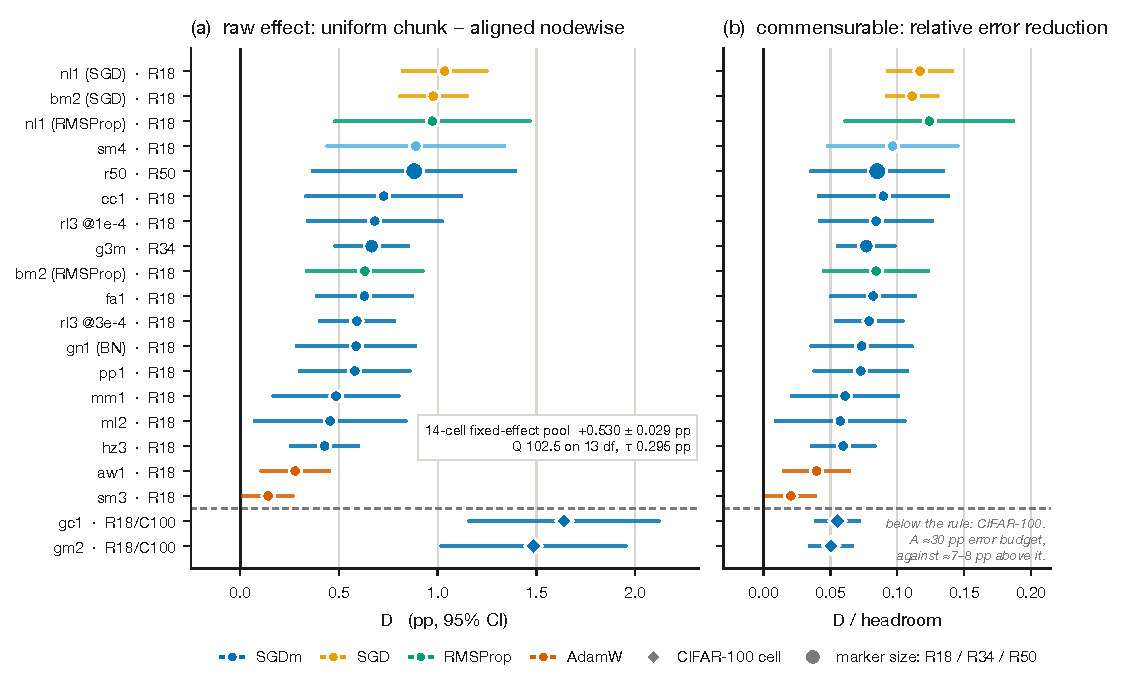
\includegraphics[width=\linewidth]{figures/f1_forest_D.pdf}
\caption{\textbf{$\Dstat$ in every count-matched cell, and the same effect made
commensurable.} (a) $\Dstat = $ uniform chunk $-$ architecture-aligned \arm{nodewise},
\plateau, taken within batch, with 95\% intervals from the Welch standard error of
Table~\ref{tab:D}. Colour is the base optimiser, marker shape the dataset, marker size the
network depth. \textbf{$\Dstat$ is positive in every one of the twenty cells.} The horizontal
rule separates CIFAR-10 from CIFAR-100: the two sit on $\approx 7$--8 pp and $\approx 29$--30 pp
error budgets and a percentage point does not mean the same thing across it, so panel (a) must
not be read across the rule. (b) The same twenty contrasts as a share of the aligned arm's
remaining error, $\rho = \Dstat / (100 - \text{aligned})$ (Eq.~\ref{eq:rho}), which \emph{is}
commensurable. The ordering changes: CIFAR-100's $+1.640$ pp, the \textbf{largest} $\Dstat$ in
panel (a), is $\rho = 0.055$ --- the \textbf{fourth smallest}
of the twenty, behind \arm{sm3} (0.020), \arm{aw1} (0.040) and the other CIFAR-100 cell
\arm{gm2} (0.050). The
inset gives the fixed-effect pool over the fourteen cells that run the same ResNet-18 partition
contrast; \arm{sm4}, the one cell with a non-Lion meta-optimiser, is plotted but is not in that
pool.}
\label{fig:forest}
\end{figure}

\subsection{The heterogeneity has a candidate moderator, the base optimiser --- and a rival we
can measure but not exclude}
\label{sec:moderator}

Restrict Table~\ref{tab:D} to the fourteen cells that run the same ResNet-18 partition contrast
(\arm{nodewise} $\rightarrow$ \arm{chunk777}, count-matched to $+1$ group on 14{,}420; rows
1--4, 6--12 and 17--19) so that the contrast itself is held fixed. \arm{sm4} (row 20) is
\textbf{excluded from every pool in this section} by its own registered scope note, which forbids
pooling it with \arm{aw1} or \arm{sm3}; it runs a different meta-optimiser and is treated in
\S\ref{sec:normalisation}. Those fourteen are heterogeneous. Because $\tau > 0$ the
\textbf{random-effects} (DerSimonian--Laird) pool is the honest summary of them, and it is
$\mathbf{+0.611 \pm 0.087}$ pp, 95\% CI $[+0.441, +0.782]$. The \textbf{fixed-effect} pool ---
which is what Figure~\ref{fig:forest}'s inset, the endpoint table below and every other
``pooled $\Dstat$'' in this paper report --- is $+0.530 \pm 0.029$, and that interval covers the
truth 65\% of the time rather than 95\%: its calibrated 95\% half-width is 0.089 pp, not the
0.058 that $1.96\,\se$ gives (\S\ref{sec:threats} T13). We print both and label which is which
rather than quietly switching.

\begin{quote}
\textbf{$Q = 102.47$ on 13 df}: $p = 5.5\times10^{-16}$ against $\chi^2_{13}$, which is
\textbf{not the distribution this $Q$ has}, and \textbf{Monte-Carlo $p = 0.013$} against the
distribution it does have (0.002 under the common-sd null; \S\ref{sec:threats} T13). The null
$Q$ on 13 df has mean 26.9, median 21.4 and 95th percentile 62.4, against $\chi^2_{13}$'s 13,
12.3 and 22.4. DerSimonian--Laird \textbf{$\tau = 0.295$ pp} against an rms measurement $\se$
of \textbf{0.143 pp}, i.e.\ $I^2 = 87\%$ --- \textbf{both of these are upper bounds}, because
\eqref{eq:Q} subtracts $k - 1 = 13$ where the null mean is 26.9; recentred there they read
$\tau = 0.271$ pp and $I^2 = 74\%$ (0.280 pp and 79\% under the common-sd null). We keep the
standard estimator and label it rather than substituting one of our own.
\end{quote}

Three of the fourteen were not available to the previous version of this paper. Two are \arm{bm2}, the registered
replication of \S\ref{sec:inflight}'s R3, and they are quoted from its scorer,
\texttt{analysis/c97\_bm2\_score.py}, run unedited on the cluster where its probe records live
(RULE 16; the box gate R0.5 is measured on \arm{bm2}'s own twelve probe dirs, $T = 10{,}000$
records, all rails 0.0000):

\begin{quote}\ttfamily\footnotesize
D'\_SGD~~base SGD~~+0.9780 +- 0.0858~~t 11.40~~3v3~~-> REPLICATES\\
D'\_RMS~~base RMSProp~~+0.6313 +- 0.1492~~t 4.23~~3v3~~-> REPLICATES\\
SGD~~~~~~nl1 +1.0353+-0.1085 | bm2 +0.9780+-0.0858 -> pool +1.0000 +- 0.0673~~Q 0.172 on 1 df
-> REPLICATED\\
RMSProp~~nl1 +0.9733+-0.2515 | bm2 +0.6313+-0.1492 -> pool +0.7204 +- 0.1283~~Q 1.367 on 1 df
-> REPLICATED
\end{quote}

\arm{bm2} is one submission of four arms at three \textbf{fresh} seeds (3, 4, 5 against
\arm{nl1}'s 0, 1, 2), at \arm{nl1}'s own cell read off \arm{nl1}'s own \texttt{ARGS:} line.
Independence is bought twice --- a separate submission, so the batch random effect is resampled,
and fresh seeds, so the \arm{ml2} failure mode cannot recur. The third is \arm{sm3}, whose twelve
rows are now in the deposited run table and which --- under RULE 20, on its own \texttt{ARGS:}
line --- ran AdamW\,+\,Lion and is an independent replicate of \arm{aw1}
(\S\ref{sec:silent-failures}). \arm{nl1} is \textbf{combined with} \arm{bm2} and is not
overwritten, and the two \arm{bm2} bases are \textbf{never pooled with each other}, both of which
the scorer's R5 forbids.

Split the fourteen by the base optimiser, the axis \S\ref{sec:normalisation} was already looking
at:

\begin{center}
\footnotesize
\setlength{\tabcolsep}{4pt}
\begin{tabular}{@{}llrrll@{}}
\toprule
base optimiser & base state, from the runs' own \texttt{ARGS} line & cells & batches &
  pooled $\Dstat$ (pp) & within-level $Q$/df ($\chi^2$ $p$; MC $p$) \\
\midrule
SGD     & no momentum, no second moment & 2 & 2 & $\mathbf{+1.000 \pm 0.067}$ & 0.17 / 1 (0.68; \textbf{0.70}) \\
RMSProp & second moment 0.999, no momentum & 2 & 2 & $\mathbf{+0.720 \pm 0.128}$ & 1.37 / 1 (0.24; \textbf{0.30}) \\
SGDm    & momentum 0.99, no second moment & 8 & 7 & $\mathbf{+0.556 \pm 0.045}$ & 4.21 / 7 (0.76; \textbf{0.86}) \\
AdamW   & momentum 0.9 + second moment 0.999 & 2 & 2 & $\mathbf{+0.189 \pm 0.052}$ & 1.61 / 1 (0.20; \textbf{0.25}) \\
\bottomrule
\end{tabular}
\end{center}

\textbf{Between base optimisers, $Q = 95.12$ on 3 df --- 92.8\% of the total; within levels,
$Q = 7.36$ on 10 df.} Both $p$-values are printed twice throughout, because the first of them is
computed against the wrong reference: between-base $p = 1.7\times10^{-20}$ against $\chi^2_3$
and \textbf{Monte-Carlo $p = 0.005$} against the distribution that $Q$ actually has (0.0007 under
the common-sd null), within-level $p = 0.69$ against $\chi^2_{10}$ and Monte-Carlo $p = 0.86$.
\textbf{The direction of every one of these corrections is the same}: heterogeneity is far less
resolved than $\chi^2$ says, and homogeneity is more so. \S\ref{sec:threats} T13 gives the
simulation, and the weight-free permutation two paragraphs below is what this subsection's
central claim now rests on. \textbf{Every level of this moderator
now rests on at least two independent submissions.} That is new, and it is the single most
important thing \arm{bm2} and the \arm{sm3} ingest bought. Before stating what the decomposition
does and does not license, we state the arithmetic that limits it, because a referee will find it
otherwise.

\paragraph{The share is a property of the grouping, not of the label.}
A level with one cell contributes $Q = 0$ by construction. In the eleven-cell pool of the
previous version of this paper, \emph{three} of the four levels were singletons, so $Q_{\mathrm{between}}$ was
identically $Q_{\mathrm{total}}$ minus the eight-cell SGDm $Q$ --- $36.4048 - 4.2060 = 32.1988$
--- for \textbf{any} partition isolating those three cells, whatever it called them, and ``88\%
is one identified moderator'' therefore claimed more than the number could carry. On fourteen
cells no level is a singleton: 3.15 of the present 7.36 within-level $Q$ sits, on 3 df, in levels
that previously had none, and those 3 df were a test the label could have failed --- the scorer's
registered line is $Q > 3.841 \Rightarrow$ the level is not a stable quantity --- and did not.
The base partition is now a \textbf{restriction the data could have rejected}, and it did not
reject it: all four levels are homogeneous, $\chi^2$ $p$ 0.20--0.76 and Monte-Carlo $p$
0.25--0.86. (That registered rule is itself mis-sized for the same reason: simulated, $Q > 3.841$
fires on a homogeneous two-cell level 10\% of the time and not 5\%, and the size-0.05 critical
value is 6.22. A level that does not fire it is therefore \emph{stronger} evidence of
homogeneity than the rule claims, not weaker.) Over all 45{,}045 partitions of the fourteen cells
with the realised shape $\{8, 2, 2, 2\}$, the base-optimiser partition ranks 14th
(permutation $p = 0.00031$, against a median share of 0.333 and a maximum of 0.957).
Leave-one-cell-out over the fourteen gives 89.6\% to 95.7\%.

\textbf{The weight-free version of that permutation, which is what this subsection now rests on.}
The rank-14 test above permutes labels but still scores each partition by a \emph{weighted} share
of $Q$, so it inherits the $\se_i$ and their two-to-four degrees of freedom. Scoring the same
45{,}045 partitions by the \textbf{unweighted} between-group share of the fourteen $\Dstat$'s
variance removes the standard errors from the test altogether:
\begin{quote}
$\eta^2 = \mathbf{0.840}$ for the base-optimiser partition, \textbf{rank 9 of 45{,}045}, exact
$p = \mathbf{0.00020}$, against a null median of 0.200 and a maximum of 0.894.
\end{quote}
\textbf{This is the load-bearing statistic for the moderator claim from here on}, because it
does not depend on the $\se$ estimates at all and so is untouched by \S\ref{sec:threats} T13.
It is an exact enumeration, not a sample, so it carries no Monte-Carlo error; and run on the
weighted share it reproduces the published rank 14 and $p = 0.00031$ above, which is how we know
the enumeration is the paper's own. Note what it does and does not say: like the rank-14 test it
is conditional on the observed spread of the fourteen $\Dstat$ and asks only whether \emph{this
partition} of them is special. Whether there is any spread to partition is the separate question
$Q$ answers, and calibrated, $Q$ answers it at $p = 0.013$.

\paragraph{The rival label, measured.}
The variable most likely to induce this grouping by accident is batch identity, because the two
partitions very nearly coincide: the fourteen cells fall into eleven submissions, so a four-way
split on the base optimiser is close to a split on which submission a cell came from. (An earlier
version of this paragraph motivated the test instead with a batch random effect of
$F(62,85) = 5.47$ carried from the project record. That statistic is \textbf{withdrawn} --- it
does not re-derive under any cell definition we could build; see \S\ref{sec:variance} and
Appendix~\ref{app:discrepancy}.3 --- and the test below never depended on it. The rival is worth
testing because of how the design is confounded, not because of a variance estimate.)
Partitioning the fourteen cells by submission gives eleven levels,
between $Q = 98.16$ on 10 df --- \textbf{95.8\%, more than the base optimiser's 92.8\%}. Nesting
both inside their common refinement (base $\times$ batch, thirteen levels, within $Q = 0.21$ on
1 df) separates them:

\begin{quote}
Adding \textbf{batch given base} costs $\mathbf{\Delta Q = 7.15}$ \textbf{on 9 df, $p = 0.62$}
--- once you know the base optimiser, which submission a cell came from explains nothing further.
Adding \textbf{base given batch} costs $\mathbf{\Delta Q = 4.11}$ \textbf{on 2 df, $p = 0.13$}
--- knowing the base optimiser does add something beyond submission identity, but not at
$p < 0.05$.
\end{quote}

On the eleven-cell pool the second of those two numbers was $\Delta Q = 0.05$ on 1 df,
$p = 0.82$: base added nothing whatsoever beyond batch. That is what \arm{bm2} bought, and it is
a smaller purchase than ``the moderator is now replicated at every level'' would suggest --- the
conditional test is \textbf{unchanged} by the \arm{sm3} ingest, because \arm{sm3} is its own
batch as well as an AdamW cell. Nor is the base optimiser the best-fitting partition: cutting the
same fourteen cells post-hoc into four contiguous groups in $\Dstat$ order removes
\textbf{97.5\%} of $Q$, and the best partition of the realised shape removes 95.7\%. Neither is a
competitor, because both are chosen on the outcome; they are quoted so that ``92.8\%'' is read as
\emph{this axis removes almost all of the heterogeneity}, not as \emph{no other partition could}.
Two axes that are not chosen on the outcome remove essentially none of it: $\beta$-box 0.7\%,
meta-stepsize 1.2\%, budget 1.5\%. \textbf{The base optimiser is the parsimonious description of
these fourteen cells --- four levels lose nothing against eleven --- and it is not yet separated
from the nuisance variable it co-varies with.} We therefore write ``candidate moderator'', not
``identified moderator'', and we do not write that the base optimiser \emph{carries} or
\emph{explains} the heterogeneity.

\paragraph{The one out-of-sample test that exists.}
\arm{bm2} is the first occasion on which the moderator made a prediction before the data existed.
\arm{nl1}'s levels predicted $+1.0353$ (SGD) and $+0.9733$ (RMSProp); the corpus mean predicted
$+0.5707$ for both. Observed: $+0.9780$ and $+0.6313$, prediction errors $-0.057$ ($z\ -0.41$)
and $-0.342$ ($z\ -1.17$). The base-level predictor's RMSE is 0.245 pp against the grand mean's
0.291 pp --- \textbf{29\% of the squared prediction error removed, on two points} --- and on
RMSProp alone the grand mean was the better predictor. This is offered as the direction the
evidence points, not as a validated rule; \S\ref{sec:prediction}'s out-of-sample null, whose unit
is the design point and whose predictors are continuous, is unaffected.

The remaining within-level residual is not resolvable at all:

\begin{quote}
Over the eight SGDm cells --- \textbf{seven separate submissions, two meta-stepsizes
($10^{-4}$, $3\times10^{-4}$), two budgets (100 and 300 epochs), three $\beta$-boxes and two
clusters} --- the pool is $\mathbf{+0.556 \pm 0.045}$ with $\mathbf{Q = 4.21}$ \textbf{on 7 df,
$I^2 = 0\%$, $\tau = 0.000$}. $\chi^2_7$ puts that $Q$ at $p = 0.76$; \textbf{its own simulated
null, whose median is 9.4, puts it at Monte-Carlo $p = 0.86$ and at the 14th percentile}
(\S\ref{sec:threats} T13), so the homogeneity claim holds and the reference it used to be stated
against did not. The one-sided 95\% $Q$-profile upper limit on $\tau$ is \textbf{0.109 pp}
against $\chi^2_7$ and \textbf{0.097 pp} when the profile is simulated at each trial $\tau$ ---
\textbf{the one quantity in this subsection the $\chi^2$ reference gets wrong in our
disfavour} --- and both are below the 0.146 pp rms measurement $\se$ of the cells themselves. The
pool's own interval is the one that moves the other way: $\pm 1.96\,\se$ is $\pm 0.088$ pp and
covers 73\%, and the calibrated 95\% half-width is $\pm 0.121$ pp.
\end{quote}

Four of those eight are submissions of the \emph{identical} configuration --- \arm{cc1},
\arm{mm1}, \arm{pp1} and the BatchNorm arm of \arm{gn1} --- and they land
at $+0.727$, $+0.485$, $+0.581$ and $+0.587$, $Q = 0.88$ on 3 df, $p = 0.83$. \textbf{They are
not four independent replications and we no longer describe them as such.} Between them the four
draw thirteen cell-seeds from \textbf{six} distinct seeds: \arm{mm1}, \arm{pp1} and \arm{gn1} all
use seeds 0--2, \arm{gn1} adds seed 3, and \arm{cc1} uses 3--5. The overlap is exact rather than
nominal --- \arm{gn1-bn-ch-s0}, \arm{mm1-ch-s0} and \arm{pp1-ch-s0} are the same experiment, the
same effective argument line after last-wins resolution with the same \texttt{ENV} and the same
\texttt{--seed}, as are their \arm{nodewise} partners (which \arm{bn1} and \arm{tw0} also re-run),
and \arm{cc1-*-s3} is the same experiment as \arm{gn1-bn-*-s3}. The largest mutually seed-disjoint
subset of the four is \textbf{two} cells: \arm{cc1} against either \arm{mm1} or \arm{pp1}, which
agree at $Q = 0.88$ and $Q = 0.36$, each on 1 df. Restricted to the three seeds they share,
\arm{mm1}, \arm{pp1} and \arm{gn1} read $+0.485$, $+0.581$ and $+0.408$ --- a 0.173 pp spread over
three measurements of one six-run experiment.

\textbf{What their agreement measures is therefore re-measurement of a fixed seed set across
batches, not replication across seeds}, and \S\ref{sec:variance} is where its worth is settled:
with the batch variance component withdrawn (sd$_{\text{batch}} = 0.000$ pp, $F(39,172) = 0.71$),
a second submission at the same seeds is a rerun, not a replicate. $Q = 0.88$ on 3 df says that
$\Dstat$ does not move between reruns, which is worth knowing and is not nothing; it does not say
that $\Dstat$ survives a change of seed. The one comparison in this pool that does say that is
\arm{cc1} against \arm{mm1} or \arm{pp1}, and it agrees. The within-SGDm residual inherits the
same caveat and we flag it rather than let the reader find it: four of the eight cells re-measure
one seed set, which can only lower $Q$, so \textbf{$Q = 4.21$ on 7 df is an upper bound on
homogeneity's evidence, not a neutral test.}
Leave-one-cell-out over the eight never resolves heterogeneity ($Q$ 1.21--4.17 on 6 df, pool
$+0.544$ to $+0.603$; $\tau = 0.000$ in all eight subsets), and no other axis available inside
the subset competes with the base: $\beta$-box $Q = 0.76/2$ ($p\ 0.68$), meta-stepsize
$Q = 0.68/1$ ($p\ 0.41$), budget $Q = 2.99/1$ ($p\ 0.084$), cluster account $Q = 0.76/1$
($p\ 0.38$).

\textbf{These fourteen cells are not one configuration, and we do not call them one.} They span
three step-size clip boxes --- $-15{:}{-}2.3026$ (10 cells), $-30{:}9.0$ (3),
$-25{:}{-}2.3026$ (1) --- and \texttt{analysis/c87\_rl3\_score.py}'s registered header forbids
pooling across boxes, on the ground that a box change moves the optimiser and not merely the
instrument. We pool anyway; \S\ref{sec:registration} lists this as one of the paper's three
departures from a registered scorer. \textbf{The measurement that justifies it moves with the
cell set, and we report that rather than only the state that flatters us.} On the eleven-cell
pool, partitioning $Q$ by box gave between-box $Q = 1.08$ on 2 df ($p = 0.58$) against within-box
$Q = 35.32$ on 8 df; on the thirteen-cell intermediate pool that contained \arm{bm2} but not
\arm{sm3} it rose to \textbf{5.14 on 2 df ($p = 0.077$)}, because both \arm{bm2} cells sit in
$-15{:}{-}2.3026$; on the fourteen cells above it is \textbf{0.69 on 2 df ($p = 0.71$)}. That
figure is unstable because the box axis has become partly confounded with the axis under study
--- all four non-SGDm cells sit in one box --- so we do not rest the pooling on it. The test that
is not confounded is the one taken inside a single base: over the eight SGDm cells, which between
them span all three boxes, between-box $Q$ is \textbf{0.76 on 2 df, $p = 0.68$}, with pools
$+0.582 \pm 0.080$ ($-15$), $+0.629 \pm 0.123$ ($-25$) and $+0.523 \pm 0.060$ ($-30$).
\textbf{That} is what the pooling rests on. A $\beta$-box column is carried in Table~\ref{tab:D}
and in Appendix~\ref{app:arms} so the reader can redo either split.

So the finding is not ``$\Dstat$ varies for reasons we cannot attribute'', and it is not ``one
identified moderator'' either. It is:

\begin{quote}
\textbf{Inside a base optimiser, $\Dstat$ does not move.} Under SGDm it is $+0.556 \pm 0.045$
pp across seven submissions, two meta-stepsizes, two budgets, three $\beta$-boxes and two
clusters ($Q$ 4.21 / 7, $\tau = 0.000$); under SGD it is $+1.000 \pm 0.067$, under RMSProp
$+0.720 \pm 0.128$ and under AdamW with a Lion meta $+0.189 \pm 0.052$, each across two
independent submissions ($Q$ 0.17, 1.37 and 1.61, each on 1 df).
\textbf{Between base optimisers the pooled level moves by a factor of 5.3}, and a four-way split
on that axis leaves the fourteen cells internally homogeneous while accounting for 92.8\% of
their Cochran $Q$. \textbf{What we cannot say is that the base optimiser is the cause.} The same
92.8\% would be earned by any covariate inducing the same grouping; the grouping's chief rival,
batch identity, accounts for 95.8\%; and conditioning one on the other leaves base adding
$\Delta Q$ 4.11 on 2 df, $p$ 0.13 --- real, and not resolved.
\end{quote}

\paragraph{Say which denominator.}
The between-base $Q$ of 95.12 is 92.8\% of the fourteen-cell $Q$ of 102.47, which is the pool the
decomposition is computed on. The figure is not sensitive to the two cells whose inclusion is
arguable: adding \arm{ml2} at its corrected $\se$ gives 92.6\% (pool $+0.528 \pm 0.029$,
$Q$ 102.61 / 14, between 95.01 / 3), and restoring the withdrawn GroupNorm arm as a fifth level
gives 93.2\% (pool $+0.515 \pm 0.029$, $Q$ 107.97 / 14, between 100.61 / 4). The corresponding
figure on the previous version's eleven cells was 88.4\% of a $Q$ of 36.40, and against the legacy
twelve-cell pool that contained the GroupNorm cell it was 74.6\% --- the ``$\approx 75\%$'' that
earlier versions of this work quoted. All are true of different denominators; none may be quoted
without naming its own.

\paragraph{The endpoint, varied --- and the part of this subsection that does not survive it.}
Everything above is computed on \plateau{}, and \S\ref{sec:metric} concedes, as the sixth of its
selection items, that \plateau{} was made primary \emph{after} the 20-epoch column produced two
withdrawn headlines: the choice has a mechanical justification, it has been applied uniformly
since, and \textbf{it was not fixed before the first analysis}. A decomposition of between-cell
heterogeneity is a statement about a \emph{spread}, and a spread is a property of the endpoint at
least as much as of the runs. We therefore re-derive this entire subsection on the three other
end-of-training endpoints the deposited run table already carries --- the 20-epoch
\texttt{plateau} column, the best test epoch \texttt{best\_test}, and the last test epoch
\texttt{final\_test} --- holding the admissibility gate of \eqref{eq:adm}, the arm definitions,
the \texttt{dup\_group} collapse and the fourteen-cell pool \textbf{fixed}, and varying only the
column that is read. This is not \S\ref{sec:threats} T10, which varies the row filter at a fixed
endpoint; it is the other axis, and no previous version of this paper reported the decomposition
on any endpoint but \plateau{}.

\begin{center}
\footnotesize
\begin{tabular}{@{}lrrrrrrrr@{}}
\toprule
endpoint & pooled $\Dstat$ & $Q$ / 13 df & $p$ ($\chi^2_{13}$) & MC $p$ & $\tau$ &
  between-base $Q$ & share & $\Dstat > 0$ \\
\midrule
\plateau{} \emph{(primary)}         & $+0.530 \pm 0.029$ & 102.47 & $5.5\times10^{-16}$ & \textbf{0.013} & 0.295 & 95.12 & \textbf{92.8\%} & 20 / 20 \\
\texttt{plateau} \emph{(20-epoch)}  & $+0.449 \pm 0.024$ &  29.37 & 0.0058              & \textbf{0.24}  & 0.101 & 18.36 & 62.5\%          & 20 / 20 \\
\texttt{best\_test}                 & $+0.396 \pm 0.025$ &   \textbf{9.87} & \textbf{0.70} & \textbf{0.90} & \textbf{0.000} & 3.70 & 37.5\% & 20 / 20 \\
\texttt{final\_test}                & $+0.614 \pm 0.043$ &  39.91 & $1.4\times10^{-4}$  & \textbf{0.16}  & 0.251 & 34.66 & 86.8\%          & \textbf{19 / 20} \\
\bottomrule
\end{tabular}
\end{center}
\noindent\emph{Columns: the \textbf{fixed-effect} pooled $\Dstat$ in pp over the fourteen
cells; Cochran $Q$ on 13 df; its $p$ against $\chi^2_{13}$ and its Monte-Carlo $p$ against the
distribution $Q$ actually has at these degrees of freedom (per-cell null; the common-sd null
gives 0.002, 0.19, 0.88 and 0.080); DerSimonian--Laird $\tau$ in pp, an upper bound for the same
reason; the between-base component of $Q$ on 3 df; its share of $Q$; and how many of the twenty
count-matched cells of Table~\ref{tab:D} are positive.}

\noindent \textbf{The MC column is the one that means anything, and it changes the reading of
three rows out of four} (\S\ref{sec:threats} T13). The random-effects pools of the same four
rows are $+0.611 \pm 0.087$, $+0.480 \pm 0.038$, $+0.396 \pm 0.025$ and $+0.674 \pm 0.097$ pp;
the between-base $Q$'s Monte-Carlo $p$'s are 0.005, 0.099, 0.60 and 0.025; and the weight-free
permutation, which uses no $\se$ at all and therefore survives all of this untouched, gives
$\eta^2$ 0.840, 0.800, 0.276 and 0.670 at exact $p$ 0.00020, 0.00029, 0.34 and 0.0076.

\noindent The same four endpoints, split by base optimiser --- the table this subsection is built
on, recomputed three more times:

\begin{center}
\small
\begin{tabular}{@{}lrrrrl@{}}
\toprule
endpoint & SGD & RMSProp & SGDm & AdamW & rank order, largest to smallest \\
\midrule
\plateau{} \emph{(primary)}        & $+1.000$ & $+0.720$ & $+0.556$ & $+0.189$ & SGD, RMSProp, SGDm, AdamW \\
\texttt{plateau} \emph{(20-epoch)} & $+0.737$ & $+0.634$ & $+0.438$ & $+0.315$ & SGD, RMSProp, SGDm, AdamW \\
\texttt{best\_test}                & $+0.432$ & $+0.386$ & $+0.411$ & $+0.261$ & SGD, SGDm, RMSProp, AdamW \\
\texttt{final\_test}               & $+0.139$ & $+1.518$ & $+0.588$ & $+0.420$ & \textbf{RMSProp, SGDm, AdamW, SGD} \\
\bottomrule
\end{tabular}
\end{center}

Three readings, stated plainly rather than buried.

\begin{enumerate}
\item \textbf{On \texttt{best\_test} there is no heterogeneity to decompose at all.} $Q = 9.87$
  on 13 df sits at the \textbf{tenth percentile of its own simulated null} (Monte-Carlo
  $p = 0.90$). ``Below its own degrees of freedom'' is the wrong way to say it --- that null's
  mean is 25.3, not 13 (\S\ref{sec:threats} T13) --- but it is right about the direction and by
  a wider margin than $\chi^2_{13}$'s $p = 0.70$ suggested: $I^2 = 0\%$, DerSimonian--Laird
  $\tau = 0.000$, and between base optimisers $Q$ is 3.70 on 3 df ($p = 0.30$ against $\chi^2_3$,
  Monte-Carlo $p = 0.60$). The weight-free permutation agrees and is the cleanest statement of it:
  $\eta^2 = 0.276$, rank 15{,}248 of 45{,}045, exact $p = 0.34$. This is not an
  error-inflation artefact --- \texttt{best\_test}'s rms measurement $\se$ over the fourteen cells
  is 0.137 pp against \plateau{}'s 0.143 pp, within 5\% --- it is that the between-cell spread is
  gone: the sd of the fourteen $\Dstat$ is 0.084 pp on \texttt{best\_test} against 0.255 pp on
  \plateau{}, i.e.\ \emph{smaller than the measurement error}. On that endpoint the base-optimiser
  decomposition is not a weaker result. It is not a result.
\item \textbf{The base-level ordering inverts between \plateau{} and \texttt{final\_test}.} SGD is
  the largest of the four levels on \plateau{} ($+1.000$) and the \emph{smallest} on
  \texttt{final\_test} ($+0.139$), while RMSProp moves from second to first. The factor of 5.3
  quoted above is 2.3 on the 20-epoch column, 1.7 on \texttt{best\_test} --- where the four levels
  sit inside a 0.17 pp band that no pair of them resolves --- and 10.9 on \texttt{final\_test}.
  The momentum / second-moment $2 \times 2$ of the next paragraph is a reading of the \plateau{}
  ordering and does not survive either single-epoch endpoint.
\item \textbf{The endpoint this project chose is the one on which the decomposition is
  strongest.} A referee is entitled to write that sentence, so we write it first: of the four,
  \plateau{} maximises $Q$, maximises $\tau$ and maximises the between-base share.
\item \textbf{Calibrated, \plateau{} is the only one of the four with resolved heterogeneity at
  all.} Referring each row's $Q$ to its own simulated null instead of to $\chi^2_{13}$
  (\S\ref{sec:threats} T13) gives Monte-Carlo $p$ 0.013, 0.24, 0.90 and 0.16. The 20-epoch
  column's $p = 0.0058$ and \texttt{final\_test}'s $p = 1.4\times10^{-4}$ \textbf{do not
  survive the correct reference}; \plateau{}'s $5.5\times10^{-16}$ does, at $p = 0.013$. This
  makes item 3 sharper rather than softer --- on three of the four endpoints there is no resolved
  spread for any moderator to explain --- and it is a self-criticism, so we print it in the same
  list as the other three rather than in a footnote. The claim it does \emph{not} touch is
  \S\ref{sec:primary}'s: the sign, which is 20 / 20 on three endpoints and 19 / 20 on the
  fourth, is a per-cell quantity and is not pooled.
\end{enumerate}

\textbf{What survives the change of endpoint is \S\ref{sec:primary}'s measurement, not this
subsection's decomposition.} The fourteen-cell pool is positive and of one order on all four
(fixed-effect pools $+0.396$ to $+0.614$ pp; random-effects $+0.396$ to $+0.674$), and the
count-matched sign result of Table~\ref{tab:D} reads
\textbf{20 / 20, 20 / 20, 20 / 20 and 19 / 20} cells. The single exception is \arm{bm2} (SGD) on
\texttt{final\_test}: $\Dstat = -0.073 \pm 0.500$, $t = -0.15$. \textbf{That is a cell the
endpoint cannot read, not a cell that reverses.} \texttt{final\_test} is one epoch's evaluation,
and inside \arm{bm2}'s two arms the sd of that single reading is 0.467 and 0.729 pp against 0.127
and 0.077 pp for \plateau{}, so the cell's $\se$ inflates 5.8-fold, from 0.086 to 0.500 pp, and
$|\Dstat|$ falls well inside it; on the same six runs \plateau{} reads $+0.978 \pm 0.086$,
$t\ 11.40$, the most resolved cell in Table~\ref{tab:D}. The resolution loss is corpus-wide and
not peculiar to that cell: of the twenty, 18 are resolved at $t \ge 3$ on \plateau{} and 20 on the
20-epoch column, against 11 on \texttt{best\_test} and 7 on \texttt{final\_test}, and the rms
measurement $\se$ on \texttt{final\_test} is $2.5\times$ \plateau{}'s. \textbf{The sign is what
survives; the resolution and the decomposition are not endpoint-free.}

\paragraph{The conditional form, which is the form this claim should have carried from the start.}
\S\ref{sec:contributions}'s third contribution is therefore not ``the heterogeneity in $\Dstat$
has a base-optimiser structure''. It is:

\begin{quote}
\textbf{On the 5-epoch plateau endpoint --- an endpoint this project chose after seeing data
(\S\ref{sec:metric}, selection item 6) --- the heterogeneity in $\Dstat$ has a base-optimiser
structure accounting for 92.8\% of Cochran $Q$. On the last-epoch endpoint that structure is
weaker but present (86.8\%), with the level ordering inverted. On the best-epoch endpoint there
is no heterogeneity to decompose.}
\end{quote}

We are not arguing that \plateau{} is wrong and one of the others right, and \textbf{we do not
change the primary metric}: \plateau{} has the mechanical justification \S\ref{sec:metric} gives,
it is the endpoint every other number in this paper is computed on, and switching endpoint to suit
a claim is precisely the failure mode \S\ref{sec:metric-column} records this project committing
twice. The defect these two tables repair is a \emph{silence}. Until this version
\texttt{best\_test} and \texttt{final\_test} appeared in this paper only as column names in
\S\ref{sec:repro}'s schema listing, so a reader had no way to learn that the third contribution is
conditional on a post-hoc choice while the first is not. \S\ref{sec:threats} T10 carries the
pointer, and every number in both tables is asserted by
\texttt{python3 analysis/c98\_reproduce.py -{}-metricsens}.

\paragraph{What we may not conclude from the direction.}
The four levels arrange themselves as a $2 \times 2$ in the base optimiser's own
state: the two levels whose base carries \textbf{no momentum term} (SGD, RMSProp) sit at
$+1.000$ and $+0.720$, and the two that carry one (SGDm, AdamW) at $+0.556$ and $+0.189$. As
contrasts on the four level pools, the momentum main effect is $\mathbf{-0.488 \pm 0.080}$
($z\ -6.09$) and the second-moment main effect $\mathbf{-0.323 \pm 0.080}$ ($z\ -4.03$), with an
interaction of $-0.087 \pm 0.160$ ($z\ -0.54$) that the design cannot resolve.

\textbf{Both main effects now resolve, and that is a change from the eleven-cell reading}, where
the second-moment effect was $-0.169 \pm 0.145$ ($z\ -1.16$) and we drew a contrast between a
resolved momentum effect and an unresolved normalisation one. With \arm{bm2} and \arm{sm3} in the
pools that contrast is gone, and \S\ref{sec:normalisation} withdraws the sentence that rested on
it. What survives is that neither component \emph{alone} is the moderator: collapsing the four
levels to momentum-present / momentum-absent removes 61.1\% of $Q$ against the four-level
partition's 92.8\%, and leaves a residual $Q$ of \textbf{34.64 on 9 df} inside the
momentum-present group --- the SGDm-to-AdamW gap survives the collapse. That residual is the
largest the paper carries, and \textbf{it still does not resolve on a calibrated reference}:
$\chi^2_9$ puts it at $p\ 6.9\times10^{-5}$, its own simulated null (mean 16.5,
\S\ref{sec:threats} T13) at \textbf{Monte-Carlo $p$ 0.074}. What the collapse shows is the
\emph{share} it fails to remove, 61.1\% against 92.8\%, and that comparison needs no $p$. \textbf{The
candidate moderator is \emph{the base optimiser}, not any single component of it.}

\textbf{We still register the $2 \times 2$ as a prediction, not a
result}, for four reasons, and a referee should hold us to all four:

\begin{enumerate}
\item \textbf{The base optimiser is not separated from batch identity.} $\Delta Q = 4.11$ on
  2 df, $p = 0.13$. \arm{bm2} broke the \arm{nl1} co-dependence --- SGD and RMSProp are no longer
  two halves of a single submission --- which is why this number is 4.11 and not the 0.05 it was;
  it did not finish the job, and the \arm{sm3} ingest does not move it, because \arm{sm3} brings
  a new batch as well as a second AdamW cell.
\item \textbf{Each of the three non-SGDm levels rests on two batches, not more.} Two is enough to
  make a level's homogeneity testable --- it passes at all three ($Q$ 0.17, 1.37, 1.61 on 1 df)
  --- and not enough to estimate a between-batch variance component at that level.
\item \textbf{The momentum coefficients are not matched} (0.99 under SGDm, 0.9 under AdamW), so
  ``momentum present/absent'' is a two-point contrast in a continuous parameter.
\item \textbf{\arm{bm2} may not be asked about AdamW.} Its own registered scorer's R5 forbids
  \arm{bm2} any statement about the AdamW, SGDm or GroupNorm bases, about ResNet-34/50, about
  CIFAR-100, or about any other budget. Everything above that involves AdamW is carried by
  \arm{aw1} and \arm{sm3}.
\end{enumerate}

\paragraph{The within-batch base contrast, and a phrase we may not use.}
\arm{bm2} also reads the SGD-minus-RMSProp difference inside its own batch, which \arm{nl1} can
also do. The scorer's R3 verdict: \texttt{dD' +0.3467 +- 0.1721, t 2.01 -> AGREE WITHIN
RESOLUTION}, against \arm{nl1}'s reading of the same contrast, $+0.0620 \pm 0.2739$. The scorer
attaches the constraint in its own words --- the agreement band of 0.40 is $1.46\times$ the
planning standard error, so ``AGREE WITHIN RESOLUTION is NOT an equivalence claim and may not be
written as `identical'.'' We do not write it as identical. The two momentum-free bases are not
resolved apart by either batch, and neither batch is powered to say they are the same.

\textbf{\arm{bm2} (R3, \S\ref{sec:inflight}) was exactly the experiment this weakness named, and
it has now been scored.} It delivered two of the three repairs it was designed for: it resampled
the batch random effect at the SGD and RMSProp levels, and it broke the \arm{nl1} co-dependence
under which a batch $\times$ partition interaction peculiar to one submission would have moved
both levels together with nothing in the corpus able to see it --- such an interaction would now
have to be reproduced, at both bases and in the same direction, by an independently submitted
batch, and the between-batch spreads are $-0.057$ (SGD) and $-0.342$ (RMSProp) against a
registered agreement band of 0.5. It did not deliver the third: the base optimiser is still not
separated from batch identity ($\Delta Q$ 4.11 on 2 df, $p$ 0.13). So
``the base optimiser is a moderator of $\Dstat$'' remains a within-corpus decomposition of
fourteen measurements with one two-point out-of-sample check attached,
\textbf{not an out-of-sample prediction rule} --- which is why it does not
contradict \S\ref{sec:prediction}, where the predictors under test are continuous properties of
a configuration and the unit is the design point. It should also be read against
\S\ref{sec:registration}: \arm{nl1} is one of the five batches with no scorer registered before
its runs existed, and it still supplies half of the SGD and RMSProp levels; \arm{bm2}, which
supplies the other half, was registered before any of its runs could exist.

The one cell we removed from this pool is the GroupNorm arm of \arm{gn1} ($+0.202 \pm 0.137$):
its own registered scorer refuses to issue a verdict on a 2.862 pp difference in level against a
2.0 pp bar, so under our
own rule (\S\ref{sec:registration}) it may not be scored, and it is not reported here as a
normalisation-scheme result. For the record, keeping it as a fifth level would raise the
explained share to 93.2\% and lower the pooled $\Dstat$ to $+0.515 \pm 0.029$ --- i.e.\ the
decomposition does not depend on the exclusion; only our right to quote the cell does. Adding
\arm{ml2} as a fifteenth cell at its corrected $\se$ gives pool $+0.528 \pm 0.029$,
$Q = 102.61$ on 14 df, share 92.6\%.

The second AdamW measurement is \arm{sm3}, and it is now \textbf{in} the pool. \arm{sm3} is void
as designed (\S\ref{sec:silent-failures}) --- it declared an RMSProp meta-optimiser and, after
argparse's last-wins, ran Lion --- and is salvageable only as an independent replicate of
\arm{aw1}, which is exactly what it is used for here. Its twelve rows are in the deposited run
table, so a reader can re-derive them: $\Dstat = +0.141 \pm 0.064$ against \arm{aw1}'s
$+0.279 \pm 0.087$, a replicate spread of $+0.137 \pm 0.108$ ($z\ 1.27$), pooling to
$+0.189 \pm 0.052$ with $Q = 1.61$ on 1 df. The previous version of this paper kept \arm{sm3} out of this
decomposition on the ground that a number not in the deposited run table cannot be re-derived by
a reader running \texttt{make reproduce}; that reason expired at the ingest and we do not replace
it with another, because the alternative ground --- that \arm{sm3} is one of the five batches
\S\ref{sec:registration} names as having no scorer registered before its runs existed --- does
not distinguish it from \arm{nl1}, which supplies two cells of this same pool. The \arm{sm4}
scorer computes the same two-batch anchor its own way, as a 6 v 6 concatenation of the seeds ---
$\Dstat$ $+0.2100 \pm 0.0559$ --- and labels it, correctly, as a between-batch comparison and
\textbf{not a pooled $n$ for inference}. We use the inverse-variance pool in the table above
because that is the estimator every other level in the table uses, and we report both so the
difference is visible rather than buried.

A fifteenth same-contrast cell also exists and is excluded on a different ground: \arm{sm4}
(AdamW base, \textbf{RMSProp meta}, $\Dstat = +0.8893 \pm 0.2285$) is the corpus's only partition
cell with a non-Lion meta-optimiser. This pool is defined by a byte-identical contrast object at
a Lion meta, and pooling \arm{sm4} into it would silently convert a base-optimiser decomposition
into a base $\times$ meta one; \texttt{analysis/c97\_sm4\_score.py}'s own scope note forbids
pooling it with \arm{aw1} or \arm{sm3}. It is reported in \S\ref{sec:primary},
\S\ref{sec:prescription} and \S\ref{sec:normalisation}, not here.

\begin{figure}[htbp]
\centering
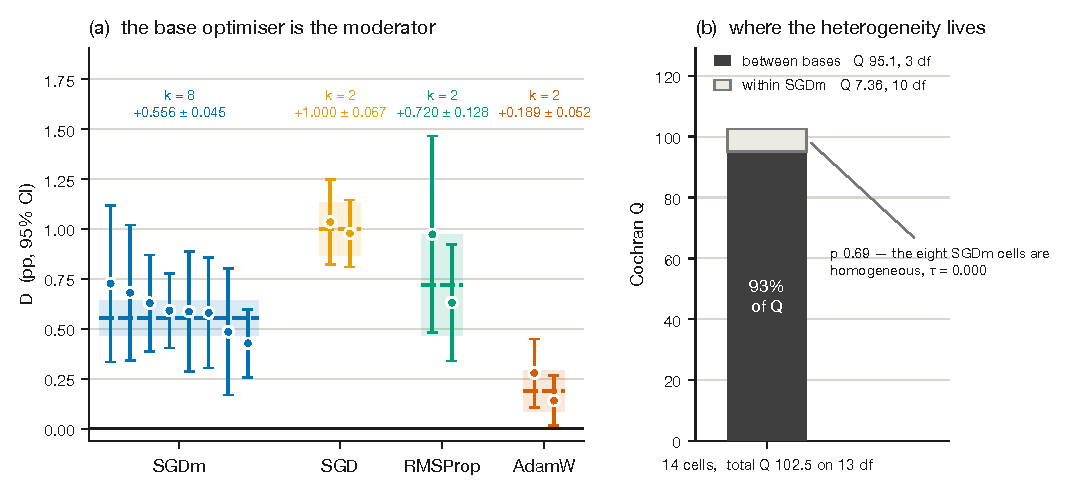
\includegraphics[width=\linewidth]{figures/f2_base_moderator.pdf}
\caption{\textbf{The heterogeneity in $\Dstat$ has a base-optimiser structure, every level of it
is now replicated, and there is a rival we can measure.} (a) The fourteen same-contrast ResNet-18
cells, grouped by base optimiser; each group's band is its own inverse-variance pool
$\pm 1.96\,\se$. Every level carries \textbf{two or more independent submissions} --- SGD
\arm{nl1} + \arm{bm2}, RMSProp \arm{nl1} + \arm{bm2}, AdamW \arm{aw1} + \arm{sm3}, SGDm seven ---
and every level is homogeneous: $Q$ 0.17 / 1, 1.37 / 1, 1.61 / 1 and 4.21 / 7 respectively, the
eight SGDm cells spanning seven separate submissions, two meta-stepsizes, two budgets and three
clip boxes at $\tau = 0.000$. (b) Partitioning the fourteen-cell Cochran $Q$ (Eq.~\ref{eq:Q}):
\textbf{95.12 of 102.47 (92.8\%) is between base optimisers}, on 3 df. \textbf{Every bare $p$ drawn
inside this figure or quoted in this caption is a $\chi^2$ value and is anticonservative}
(\S\ref{sec:threats} T13); panel (b)'s annotation carries its Monte-Carlo companion beside it: between-base $p\ 1.7\times10^{-20}$ against $\chi^2_3$ is
\textbf{Monte-Carlo $p\ 0.005$} against the distribution $Q$ actually has, and the within-level
remainder, 7.36 on 10 df at $\chi^2$ $p$ 0.69, is Monte-Carlo $p$ 0.86; the four per-level
$Q$'s are at Monte-Carlo $p$ 0.70, 0.30, 0.25 and 0.86. The weight-free statement of panel (b),
which needs no $\se$ and is what \S\ref{sec:moderator} now rests on: $\eta^2 = 0.840$, rank 9
of all 45{,}045 partitions of the realised $\{8,2,2,2\}$ shape, exact $p = 0.00020$. On the previous
version's eleven cells the same partition read 32.20 of 36.40 (88.4\%), and against the legacy
twelve-cell pool containing the withdrawn GroupNorm cell, 74.6\% --- the ``$\approx 75\%$''
figure. Every denominator must be named. The share is a property of the grouping and not of the
label --- batch identity, on eleven levels, accounts for 95.8\% --- so the panel is captioned as
a decomposition and not as an attribution; the conditional test that distinguishes them
($\Delta Q$ 4.11 on 2 df, $p$ 0.13) is in the text. \arm{sm4} is \textbf{not} in this figure: it
is the only count-matched cell with a non-Lion meta-optimiser and its registered scorer forbids
pooling it here. \textbf{Both panels are \plateau{} readings and the 92.8\% is conditional on
that endpoint}: recomputed on the corpus's three other end-of-training columns the same partition
gives 86.8\%, 62.5\% and --- on \texttt{best\_test}, where $Q$ is 9.87 on 13 df --- nothing at
all to decompose. The endpoint tables are in the text above.}
\label{fig:moderator}
\end{figure}

\subsection{Tuning each arm to its own optimum does not remove \texorpdfstring{$\Dstat$}{D}}
\label{sec:rule11}

The referee objection ranked most likely to sink this result is that $\Dstat$ compares two arms
at one arm's favourable meta-stepsize. We closed it inside one batch (\arm{rl3}, 24 runs, four
arms $\times$ $\eta \in \{10^{-4}, 3\times10^{-4}\}$ $\times$ 3 seeds). The registered scorer's
H3, verbatim:

\begin{quote}\ttfamily\footnotesize
D(ms=1e-4) = +0.681  se 0.126\\
D\_own \ \ \ \ \ = +0.591  se 0.126 \ \ \ \ \ \ \ \ (each arm at its OWN argmax)\\
dD \ \ \ \ \ \ \ \ \ = -0.090  se 0.178  t -0.51 (16 df)\\
VERDICT: RULE 11 CLOSED ON R18/CIFAR-10 -- tuning each arm to its\\
own argmax does not resolvably move D.
\end{quote}

The reportable sentence is \emph{``$\Dstat$ is unchanged at matched optima to within 0.356
pp''}. This closes the objection \textbf{on ResNet-18/CIFAR-10 and nowhere else}: no
meta-stepsize ladder exists on ResNet-34, ResNet-50 or CIFAR-100, and no ladder exists under
AdamW.

\paragraph{\texttt{dD} is an upper bound in magnitude, and here is why.}
The two rungs are $\eta \in \{10^{-4}, 3\times10^{-4}\}$ and the argmax was taken on the same
test accuracies that define $\Dstat$ (\S\ref{sec:metric}). Both arms' argmax landed on the same
rung, $\eta = 3\times10^{-4}$, so \texttt{D\_own} is itself a clean within-batch count-matched
contrast and carries no cross-arm selection. What it does carry is rung selection over two rungs
at $n = 3$, and a test-selected argmax rewards the noisier arm more: at the selected rung the
\arm{nodewise} arm has sd 0.164 against the \arm{chunk777} arm's 0.021 (\plateau, $n = 3$ each).
Selection therefore pushes \texttt{D\_own} down and pushes the measured shrinkage \texttt{dD}
away from zero, so \textbf{$-0.090 \pm 0.178$ is the largest shrinkage this two-rung ladder can
produce on this metric, not an unbiased estimate of it.} The conclusion --- that re-tuning does
not remove $\Dstat$ --- is conservative in the direction that matters, and we state it as a
bound rather than as a null.

The same batch measures $\Dstat$'s sensitivity to $\eta$ directly: $+0.681 \rightarrow +0.591$
across 0.477 decades, i.e.\ $\mathbf{-0.189}$ \textbf{pp per decade of $\eta$}, within one batch.
That is the number to use; the cross-batch cross-box value the record previously carried is
superseded.

\subsection{Alignment: a bounded null, and what it does not settle}
\label{sec:alignment}

\arm{permnode} holds \arm{nodewise}'s group \textbf{count} and its \textbf{exact per-tensor size
multiset} and randomises only \emph{which} weights share a group, within each tensor. Both
properties are measured from the allocated \texttt{beta} on the built network by the submission
script's own guard, not inherited from a comment. The contrast was registered five-way with a
symmetric band before the runs existed. The scorer's \texttt{P2}, run unedited
(\texttt{--selftest} 139/139 PASS), verbatim:

\begin{quote}\ttfamily\footnotesize
permnode<S> (m=14420, nodewise's EXACT size multiset, membership randomised)\\
\ \ \ \ 92.003 +-0.090 (n=3)\\
nodewise \ \ \ (m=14420, output channels) \ \ \ \ \ \ \ \ \ \ \ \ \ \ \ \ \ \ \ \ \ \ \ \ \ \\
\ \ \ \ 92.012 +-0.129 (n=3)\\
A = permnode - nodewise = -0.009 pp \ \ (se 0.157, t -0.06)\\
registered: A > +0.30 HURTS | (+0.15,+0.30] UND | [-0.15,+0.15] NULL |\\
\ \ \ \ \ \ \ \ \ \ \ \ [-0.30,-0.15) UND | A <= -0.30 HELPS\\
-> **NULL**
\end{quote}

In the same batch $\Dstat = +0.581 \pm 0.141$ ($t\ 4.11$) and
$B = \arm{chunk777} - \arm{permnode} = +0.590 \pm 0.107$ ($t\ 5.53$), and
$\Astat + B - \Dstat = 0$ exactly (Eq.~\ref{eq:AB}) --- a receipt on the reduction, not a
finding.

\paragraph{What the verdict licenses, printed to the same precision as the verdict.}
\texttt{NULL} is a decision about a band; it is not an estimate. The estimate is
$\Astat = -0.009$ with a 95\% interval of $\mathbf{[-0.317, +0.298]}$ \textbf{pp}, which against
this batch's own $\Dstat = +0.581$ is $\mathbf{[-55\%, +51\%]}$ \textbf{of $\Dstat$}. The
smallest alignment effect this design could have detected at 80\% power is $\mathbf{0.440}$
\textbf{pp, i.e.\ 76\% of $\Dstat$}; its power against an alignment effect equal to \emph{half}
of $\Dstat$ is $\mathbf{0.46}$. The honest reading is therefore two-sided and asymmetric in its
usefulness:

\begin{itemize}
\item \textbf{Excluded.} Alignment as the \emph{principal} carrier of $\Dstat$. An effect of
  $+0.58$ --- alignment explaining all of $\Dstat$ --- would have been detected here with
  probability 0.96, and was not.
\item \textbf{Not excluded.} Alignment as a \emph{contributing} carrier at up to roughly half of
  $\Dstat$, in either direction. The interval covers $+0.29$ and $-0.32$.
\end{itemize}

The point estimate's share of $\Dstat$, $-1.6\%$, is quoted in the project record and should be
read with the same interval attached: the share is $\mathbf{-1.6\%}$, 95\% CI
$[-55\%, +51\%]$. A ratio whose numerator is a null is not a precise quantity and we do not
present it as one.

\paragraph{A defect in our own registration, since we require it of others.}
The \texttt{NULL} band's half-width (0.15) is \textbf{narrower than the standard error the batch
achieved} (0.157). The band was set from \arm{mm1}'s effect-size scale --- deliberately, so that
the alignment and size-distribution legs would be read on one axis --- and no power calculation
was performed at the planned $n$. The consequence is computable: had the true effect been
exactly zero, this batch would have returned \texttt{NULL} on only \textbf{66\%} of realisations
and an UNDECIDED wing or worse on the other \textbf{34\%}. The verdict is therefore correctly
\emph{scored} and weakly \emph{powered}, and we report it as such. The standard error is itself
estimated on 3.6 degrees of freedom, with 95\% interval $[0.092, 0.496]$; on a Welch $t$ rather
than a normal approximation the interval on $\Astat$ widens to
$[-0.467, +0.448] = [-80\%, +77\%]$ of $\Dstat$. We print the normal-approximation interval as
the headline because it is the one registered in the project record, and the $t$ interval here so
that a reader recomputing it finds no surprise.

\paragraph{The manipulation was not inert.}
The natural objection to any null is that the knob never turned. It did. Over the same nine runs,
permuting membership moves the effective-sample-size field $N_{\mathrm{eff}}/m$ from
$0.0547 \pm 0.0010$ to $0.0414 \pm 0.0003$ --- $\mathbf{-0.0133 \pm 0.0010}$, $t\ -12.7$, which
is 70\% of the whole \arm{nodewise} $\rightarrow$ \arm{chunk777} move in that statistic --- while
moving \plateau{} by $-0.009 \pm 0.157$. This is descriptive and carries no registered direction,
and \S\ref{sec:field} has already shown that $N_{\mathrm{eff}}/m$ does \textbf{not} track
accuracy. It establishes one thing only, and that thing matters here: the permutation demonstrably
changed the optimiser's internal state, so $\Astat \approx 0$ is a statement about accuracy's
insensitivity to alignment and not about a manipulation that failed to apply.

\paragraph{Three scope limits, printed with the result rather than below it.}
\begin{enumerate}
\item \textbf{Within-layer only.} \arm{permnode} permutes \emph{inside} each tensor, so this asks
  whether an output channel is special among the same-sized subsets \textbf{of its own layer}. It
  does not test whether \emph{layer} boundaries matter. The registered scorer refuses to report
  this verdict as ``architecture is irrelevant'', and neither do we.
\item \textbf{Permutation variance is confounded with seed variance.} \arm{permnode<S>} takes
  $S =$ the run seed (\texttt{bin/c77\_permuted\_partition.sh:447}), so seeds 0--2 are three
  different permutations \emph{and} three different initialisations.
  $\se(\Astat) = 0.157$ is a compound of the two and this batch \textbf{cannot} decompose it. The
  direction is conservative --- a second variance source can only widen the interval --- but it
  means we cannot say how much of $[-0.317, +0.298]$ is draw-to-draw variation in the permutation
  itself, which is precisely the quantity the claim is about.
\item \textbf{One point in the design.} $\Astat$ is measured in \textbf{one batch, at one cell}:
  ResNet-18 / CIFAR-10 / SGDm base / Lion meta / $\eta = 10^{-4}$ / 100 epochs, with
  \arm{nodewise} read at $\eta = 10^{-4}$ rather than at its own argmax of $3\times10^{-4}$.
  $\Dstat$ is measured in twenty count-matched within-batch cells across three networks, two
  datasets, four base optimisers and two meta-optimisers. The two results are not on the same
  evidential footing and
  we do not present them as though they were.
\end{enumerate}

\subsubsection{The replication: \arm{rp1} settles limit 2, doubles the power, and confirms the
null}
\label{sec:rp1}

\arm{rp1} is \arm{pp1}'s alignment leg re-measured with the confound removed and the $n$ raised:
three fixed permutation draws (\arm{permnode101/202/303}) \textbf{fully crossed} with six fresh run
seeds (6--11), plus a six-seed \arm{nodewise} arm --- 24 jobs at \arm{pp1}'s own cell, same box,
same $\eta$, same base/meta pair, same architecture, same probe. Nothing else changes. The
permutation seed is now an explicit constant: \texttt{HF.py} builds each draw from
\texttt{torch.Generator().manual\_seed($S\cdot 1000003 + i$)} on a \emph{dedicated} generator, so
the partition depends only on $(S,\,\text{tensor index})$ and not on the global RNG that
\texttt{--seed} sets. We verified the decoupling on the runs' own \texttt{ARGS:} lines rather than
from the script header (STANDING RULE 20): each of \arm{permnode101/202/303} appears against the
full seed set 6--11, every flag appears exactly once in all 24 files, and every validity gate is
24/24 --- including \texttt{V0.4}, where all 24 probe directories report
\texttt{rec\_lo} $=$ \texttt{rec\_hi} $= 0.0000$ over $T = 10{,}000$ recorded steps, so no run
touched a clip rail.

The registered scorer \texttt{analysis/c97\_rp1\_score.py}, run \textbf{unedited}
(\texttt{--selftest} 147/147 PASS, md5 \texttt{7d21c4f5c16ccf25196fd6a5e6391fa9}) on the rebuilt
run table --- the second of two runs, the first being void and quoted nowhere
(\S\ref{sec:inflight}). Its verdict lines follow, with the printed per-verdict limits and the full
ANOVA table elided and nothing else altered:

\begin{quote}\small\ttfamily
nodewise\ \ \ \ \ m=14420\ n=6\ \ 92.066 +-0.050\\
permnode101\ \ m=14420\ n=6\ \ 92.053 +-0.050\\
permnode202\ \ m=14420\ n=6\ \ 92.030 +-0.064\\
permnode303\ \ m=14420\ n=6\ \ 92.059 +-0.050\\[2pt]
T1\ \ per-seed paired d\_s: -0.219, -0.179, +0.065, +0.052, +0.295, -0.125\\
\ \ \ \ A = permnode - nodewise = -0.018 pp\ \ (se 0.079, t -0.23 on 5 df, p 0.8248)\\
\ \ \ \ ->\ **NULL**\\
T1b se 0.0791 | 95\% CI [-0.222, +0.185] (half-width 0.203) | CI/band 1.36\\
\ \ \ \ MDE at 80\% power: 0.222 pp (normal), 0.276 pp (t, 5 df)\\
\ \ \ \ ->\ **CONSISTENT WITH NULL, UNDERPOWERED**\\
T2\ \ draw\ \ \ \ \ F(2,10) = 0.175, p 0.8423\\
\ \ \ \ ->\ THE PERMUTATION DRAW IS EXCHANGEABLE AT THIS RESOLUTION\\
\ \ \ \ run seed F(5,10) = 4.634, p 0.0190\ \ ->\ RUN SEED IS A REAL EFFECT HERE\\
\ \ \ \ sigma\_draw 0.0000 pp (TRUNCATED AT ZERO from -0.00114) | sigma\_seed 0.1000 pp\\
\ \ \ \ | sigma\_resid 0.0908 pp; smallest resolvable sigma\_draw 0.0653 pp\\
T5\ \ A / D = -2.8\%;\ \ 95\% CI = [-33.9\%, +28.3\%] of D\ \ (D pooled = +0.654 pp)
\end{quote}

\paragraph{One arithmetic note, so that nobody recomputes the interval wrongly.}
The 95\% interval above is a $\mathbf{t}$ \textbf{interval on 5 df}, not a normal one:
$t_{.975,5} = 2.5706$ times $\se = 0.0791$ gives the half-width \textbf{0.203} and the bounds
$[-0.222, +0.185]$. A reader who applies the normal factor 1.96 gets 0.155 and will not reproduce
them. The two minimum detectable effects go the other way and are printed both ways for exactly
that reason: \textbf{0.222 pp} is the normal approximation --- the same $z_{.975} + z_{.80}$
constant that produced \arm{pp1}'s quoted 0.440 pp at $\se = 0.157$, kept so that the two batches
are compared on one formula --- and \textbf{0.276 pp} is the conservative $t$ version on 5 df. We
print the mixed pair rather than silently harmonising them because harmonising would break the
comparison with \arm{pp1} that the whole subsection exists to make.

\paragraph{The binding clause did not fire, and here is the arithmetic --- and whose clause it
is.}
\textbf{This} manuscript registered in advance that \emph{if \arm{rp1} returned an interval that
still spans half of $\Dstat$, the alignment leg is to be reported as \textbf{underdetermined}
rather than as a null}. That rule is ours and not the scorer's, and we say so because we have
previously described it the other way round: the string \texttt{UNDERDETERMINED} appears
\textbf{zero} times in \texttt{analysis/c97\_rp1\_score.py}. The scorer supplies $\Astat$, its
standard error and its interval; the demotion \emph{it} registers is \texttt{T1b}, and
\texttt{T1b} \textbf{fired} (below). Ours did not, and here is why.
$\Dstat$ pooled over the two batches that measured it within batch at this configuration is
$+0.654$ pp, so half of $\Dstat$ is \textbf{0.327 pp}. The realised interval half-width is
\textbf{0.203 pp}, the normal-approximation MDE is \textbf{0.222 pp}, and the conservative
$t$-based MDE on 5 df is \textbf{0.276 pp} --- all three below 0.327. Equivalently, the interval on
$\Astat$ runs from $-33.9\%$ to $+28.3\%$ of $\Dstat$, and neither bound reaches $\pm 50\%$. The
demotion does not fire on any of these readings, so the alignment leg stands as a \textbf{null}. We
state the test rather than the conclusion alone because a rule that is only quoted when it passes
is not a rule.

\paragraph{What is now settled, and what is not.}
\begin{itemize}
\item \textbf{The permutation draw is exchangeable, and that is a finding rather than a retired
  caveat.} \textbf{Three independent draws of which weights share a group are statistically
  indistinguishable from one another}: on the balanced $3 \times 6$ grid the draw's own $F$ is
  $\mathbf{F(2,10) = 0.175}$, $\mathbf{p = 0.8423}$, and the registered scorer's verdict is
  \texttt{THE PERMUTATION DRAW IS EXCHANGEABLE AT THIS RESOLUTION}. This is a stronger statement
  than \arm{pp1}'s, and of a different kind: \arm{pp1} showed that \emph{one} arbitrary
  same-size regrouping did not move \plateau{}, which leaves open that the draw it happened to
  take was benign; \arm{rp1} shows that \emph{which} regrouping you take does not matter over
  three of them, so $\Astat$ may be read as a statement about the permutation \emph{distribution}
  rather than about one arbitrary draw. This also retires limit 2 as a measured number: the
  draw's variance component is \textbf{exactly zero} (truncated from $-0.00114$), against a
  residual sd of 0.0908 pp. The three per-draw contrasts are $-0.013 \pm 0.082$,
  $-0.036 \pm 0.105$ and $-0.007 \pm 0.062$, a spread of 0.029 pp, and \textbf{all three fall in
  the same registered band} --- so a single draw run \arm{pp1}-style would have returned the same
  verdict from this experiment. \arm{pp1}'s confound therefore inflated no variance it did not
  already carry, and $\Astat$ may be read as a statement about the permutation \emph{distribution}
  rather than about one arbitrary draw. This is registered as a null with a stated resolution,
  never as proof of zero: the smallest draw-to-draw sd this design could have resolved is
  0.0653 pp.
\item \textbf{The power roughly doubled, and that is a receipt, not a finding.} $\se(\Astat)$ falls
  from \arm{pp1}'s realised 0.157 to \textbf{0.0791} --- a ratio of $0.50\times$ against a design
  that promised $\approx 0.09$, so the design was met. The interval on $\Astat$'s share of $\Dstat$
  tightens from \arm{pp1}'s $[-55\%, +51\%]$ to $\mathbf{[-33.9\%,\ +28.3\%]}$.
\item \textbf{It is still not an equivalence claim.} \texttt{T1b} is the part of the registration
  that binds hardest, and it fires: the point estimate sits inside the $\pm 0.15$ band but the 95\%
  CI does not (CI half-width 0.203, ratio 1.36), so the correct reading is \textbf{consistent with
  null, underpowered} --- the data are equally consistent with a true zero and with an alignment
  effect up to 0.222 pp, about a third of $\Dstat$. We do not write this as ``alignment does not
  matter''. The conclusion is unchanged in \emph{kind} and stronger in \emph{degree}: alignment is
  excluded as the principal carrier of $\Dstat$, and a contribution of up to roughly a third of
  $\Dstat$ remains open where before it was up to half.
\item \textbf{The two batches are not pooled.} $\Astat$ is a within-batch quantity and the scorer
  explicitly refuses to pool \arm{rp1}'s $\Astat$ with \arm{pp1}'s; the two readings are reported
  side by side on the same registered band, which is what makes them comparable at all. The
  \texttt{T5} percentages are cross-batch and descriptive, carry the $\pm 0.25$ pp unmodelled batch
  offset, and carry no gate.
\end{itemize}

\paragraph{One disagreement with our own corpus, reported rather than smoothed.}
In this batch the run seed is a \textbf{real} effect: $F(5,10) = 4.634$, $p = 0.0190$, sd 0.100 pp.
That contradicts the corpus METHODS finding that seed is null ($F$ 1.21, $p$ 0.213; and the
batch $\times$ seed ANOVA of \S\ref{sec:discipline}, $F(30,30) = 1.50$, $p = 0.138$). We do not
reconcile the two here and we do not drop either. Two readings are available and we cannot separate
them with what we have: at one observation per cell the residual is interaction-plus-noise and not
decomposable, so a draw $\times$ seed interaction would land in the same denominator; and a single
batch's 6 seeds is a thin base from which to overturn a corpus-wide null. What it does mean
concretely is that \textbf{\arm{rp1}'s own pairing within run seed was worth doing} --- the pairing
that \texttt{T1} uses is what removes this variance from $\Astat$'s standard error. It is logged in
Appendix~\ref{app:discrepancy} as a discrepancy rather than resolved.

\paragraph{What still would settle the rest.}
Limits 1 and 3 above are untouched by \arm{rp1} and remain exactly as stated: \arm{permnode}
permutes \emph{within} each tensor, so this is a \textbf{within-layer} statement that does not test
whether layer boundaries matter; and $\Astat$ is still measured at one cell --- ResNet-18 /
CIFAR-10 / SGDm $+$ Lion / $\eta = 10^{-4}$ / 100 epochs, with \arm{nodewise} read at the inherited
$\eta$ rather than at its own argmax of $3\times10^{-4}$ --- against a $\Dstat$ measured in twenty
count-matched cells across three networks, two datasets, four base optimisers and two
meta-optimisers. \arm{rp1} doubles
the power and removes the confound; it does not broaden the design point, and we do not claim it
does.

\subsection{The prescription, and its exact scope}
\label{sec:prescription}

The practitioner's move implied by \S\ref{sec:primary} and \S\ref{sec:alignment} is: \textbf{give
each one-dimensional tensor a single step size instead of one per element.} Measured as
$\Tstat = \arm{nodewise1d} - \arm{nodewise}$ (Eq.~\ref{eq:T}), within batch, it reads as in
Table~\ref{tab:T}:

\begin{table}[htbp]
\centering
\small
\caption{$\Tstat = \arm{nodewise1d} - \arm{nodewise}$, within batch, \plateau. Twelve cells under
SGDm, SGD and RMSProp bases, every one resolved at $t \ge 3.0$; under AdamW the move is worth
nothing measurable.}
\label{tab:T}
\begin{tabular}{@{}llcrrr@{}}
\toprule
batch & network / setting & $n$ & $\Tstat$ (pp) & $\se$ & $t$ \\
\midrule
\arm{bn1} & R18 / C10 / SGDm & 3 v 3 & $+0.427$ & 0.041 & 10.43 \\
\arm{hz3}$^{\ddagger}$ & R18 / C10 / SGDm, \textbf{300 ep} & 6 v 6 & $+0.337$ & 0.069 & 4.85 \\
\arm{rl3} & R18 / C10 / SGDm, $\eta\ 3{\times}10^{-4}$ & 3 v 3 & $+0.391$ & 0.127 & 3.09 \\
\arm{ml2} & R18 / C10 / SGDm & 3 v 3 ($\times$2 reruns) & $+0.619$ & 0.176 & 3.52 \\
\arm{fa1} & R18 / C10 / SGDm, $\eta\ 3{\times}10^{-4}$ & 6 v 6 & $+0.649$ & 0.110 & 5.88 \\
\arm{nl1} & R18 / C10 / \textbf{SGD} & 3 v 3 & $+0.692$ & 0.135 & 5.12 \\
\arm{rl3} & R18 / C10 / SGDm, $\eta\ 10^{-4}$ & 3 v 3 & $+0.756$ & 0.117 & 6.45 \\
\arm{g3m} & \textbf{R34} / C10 / SGDm & 9 v 9 & $+0.758$ & 0.093 & 8.13 \\
\arm{cc1} & R18 / C10 / SGDm & 3 v 3 & $+0.816$ & 0.159 & 5.13 \\
\arm{nl1} & R18 / C10 / \textbf{RMSProp} & 3 v 3 & $+0.916$ & 0.242 & 3.79 \\
\arm{r50} & \textbf{R50} / C10 / SGDm & 3 v 3 & $+1.049$ & 0.317 & 3.31 \\
\arm{gm2} & R18 / \textbf{C100} / SGDm & 3 v 3 & $+1.363$ & 0.151 & 9.00 \\
\midrule
\arm{aw1} & R18 / C10 / \textbf{AdamW}, Lion meta & 3 v 3 & $\mathbf{+0.091}$ & 0.078 & 1.16 \\
\arm{sm3} & R18 / C10 / \textbf{AdamW}, Lion meta & 3 v 3 & $\mathbf{-0.083}$ & 0.081 & $-1.03$ \\
\arm{sm4} & R18 / C10 / \textbf{AdamW}, \textbf{RMSProp meta} & 3 v 3 & $\mathbf{+0.988}$ &
  0.231 & 4.28 \\
\bottomrule
\end{tabular}

\vspace{0.4em}
\begin{minipage}{0.92\linewidth}\footnotesize
$^{\ddagger}$ \arm{hz3} matched at 5 v 5 (seed-5 trio excluded for the clip-box and hardware
mismatch of \S\ref{sec:threats} T9): $\mathbf{+0.328 \pm 0.084}$, $t\ 3.89$. The \arm{hz3q}
quartet of \S\ref{sec:inflight} repairs that seed but is a separate registration and enters no
pool here.
The two \arm{rl3} rungs share one batch and one clip box, as Table~\ref{tab:D} rows 6 and 7
already note; they are two operating points, not two submissions. \arm{bn1} and \arm{ml2} are the
same experiment at the same seeds up to one flag Lion does not read: all twelve of their run
pairs differ only by \arm{ml2}'s last-wins residual \texttt{--normalizer-param-meta 0.999}, whose
runtime message is \texttt{args\_meta includes unnecessary attributes \{'normalizer\_param'\}}.
Their $\Tstat$'s differ by $0.192 \pm 0.181$ ($z\ 1.06$). Treat them as one measurement made
twice, not two.
\end{minipage}
\end{table}

The move costs nothing in learned parameters --- it \emph{reduces} the number of learned
quantities from 14{,}420 to
4{,}851 --- and under an SGDm, SGD or RMSProp base it is worth $\mathbf{+0.328}$ \textbf{to}
$\mathbf{+1.363}$ \textbf{pp} across \textbf{twelve} within-batch cells, \textbf{every one of
which is resolved, the weakest at $t\ 3.09$} (\arm{rl3} at $\eta = 3\times10^{-4}$; Welch
$p$ 0.037 on 3.94 df) and the strongest at $t\ 10.4$. Twelve cells is not twelve independent
measurements, and the footnotes say why: \arm{bn1} and \arm{ml2} are one experiment measured
twice, so the count of distinct experiments behind the range is \textbf{eleven}, and two further
pairs --- \arm{rl3}'s two rungs and \arm{nl1}'s two bases --- share a batch with each other rather
than sitting in separate submissions.

\textbf{The scope line is not where the previous version of this paper put it.} Under an AdamW base with a
\textbf{Lion} meta-optimiser the move is worth nothing measurable, and that now rests on two
independent batches rather than one: \arm{aw1} $+0.091 \pm 0.078$ and \arm{sm3}
$-0.083 \pm 0.081$, pooling to $\mathbf{+0.007 \pm 0.056}$ (their between-batch $Q$ is 2.39 on
1 df, so the two do not agree closely, but neither is resolved and the pool is not). Under the
\textbf{same AdamW base with an RMSProp meta-optimiser} the move is worth
$\mathbf{+0.988 \pm 0.231}$ ($t\ 4.28$) --- the largest $\Tstat$ this corpus carries
\emph{at ResNet-18 on CIFAR-10}. It is not the largest on CIFAR-10 outright: \arm{r50} reads
$+1.049 \pm 0.317$, and the superlative earlier versions of this work printed --- ``the largest
$\Tstat$ in the CIFAR-10 corpus'' --- was false of that row. It is also \plateau{}-specific: on
\texttt{best\_test} four of the eleven other ResNet-18 / CIFAR-10 cells are larger, and on
\texttt{final\_test} two are. So the
exception is not ``AdamW''. It is ``AdamW \textbf{with a Lion meta-optimiser}'', and one cell is
all the evidence there is on the other side of that line. \S\ref{sec:normalisation} develops what
this does to the mechanism story.

Two warnings travel with the \arm{sm4} row, and both come from its own registered scorer, which
classes $\Tstat$ as descriptive only. First, $\Tstat$ is \textbf{count-confounded by
construction}: it moves 0.4731 decades of group count as well as removing the size-1 tail, so it
is not a tail-removal measurement. Second, that confound is not a constant share.
Decomposing $\Tstat$ by Eq.~\ref{eq:Tid} on \arm{rl3} at $\eta = 10^{-4}$ gives
$\Tstat = +0.756 = 0.692 + 0.064$, where the \textbf{count} component is 8\% of the effect and
the tail component is the rest; the same decomposition on \arm{sm4} gives
$\Tstat = +0.988 = 0.629 + 0.359$, where the count component is \textbf{36\%}. Any account that
treats ``merge the 1-D tensors'' as purely a count reduction has the decomposition backwards, and
any account that treats the count component as negligible has it backwards at this cell.

\paragraph{The endpoint, varied --- the prescription under \S\ref{sec:moderator}'s own knife.}
\S\ref{sec:moderator} takes a knife to the base-optimiser decomposition, re-deriving it on the
three end-of-training columns the deposited run table carries besides \plateau{}, and reports
that the decomposition does not survive the change while \S\ref{sec:primary}'s sign does. That
knife has to cut here too. $\Tstat$ is this paper's only actionable recommendation --- it is the
sixth contribution, and the one a reader could act on tomorrow --- so applying the test to the
moderator and withholding it from the prescription would be exactly the selective disclosure
\S\ref{sec:moderator} was written to end. We therefore re-derive \emph{the whole of
Table~\ref{tab:T}} on \texttt{plateau} (20-epoch), \texttt{best\_test} and \texttt{final\_test},
holding the admissibility gate of \eqref{eq:adm}, the arm prefixes of Table~\ref{tab:T}, the
\texttt{dup\_group} collapse and the Welch construction \textbf{fixed}, and varying only the
column that is read.

\begin{center}
\footnotesize
\begin{tabular}{@{}lccccrr@{}}
\toprule
endpoint & $\Tstat$ over the twelve & $\Tstat > 0$ & $t \ge 3$ & rms $\se$ &
  AdamW\,+\,Lion pool & \arm{sm4} \\
\midrule
\plateau{} \emph{(primary)}        & $+0.337$ to $+1.363$ & 12 / 12 & \textbf{12 / 12} & 0.162 & $+0.007 \pm 0.056$ & $+0.988$ ($t\ 4.28$) \\
\texttt{plateau} \emph{(20-epoch)} & $+0.407$ to $+1.664$ & 12 / 12 & \textbf{12 / 12} & 0.104 & $+0.051 \pm 0.062$ & $+0.730$ ($t\ 8.70$) \\
\texttt{best\_test}                & $+0.170$ to $+1.280$ & 12 / 12 & \textbf{8 / 12}  & 0.132 & $-0.111 \pm 0.085$ & $+0.393$ ($t\ 3.89$) \\
\texttt{final\_test}               & $+0.147$ to $+1.630$ & 12 / 12 & \textbf{6 / 12}  & 0.460 & $+0.106 \pm 0.054$ & $+0.723$ ($t\ \mathbf{1.51}$) \\
\bottomrule
\end{tabular}
\end{center}
\noindent\emph{Columns: the range of $\Tstat$ over the twelve non-AdamW cells; how many of those
twelve are positive; how many are resolved at $t \ge 3$; the rms measurement $\se$ over them; the
inverse-variance pool of the two AdamW\,+\,Lion cells that fix the scope line; and \arm{sm4}, the
single cell on the other side of it.}

\textbf{The prescription survives the knife, and survives it better than
\S\ref{sec:moderator}'s decomposition did.} Three readings, in the order
\S\ref{sec:moderator} gives its own.

\begin{enumerate}
\item \textbf{The sign is endpoint-free, in every cell, on every endpoint.} All twelve
  non-AdamW cells are positive on all four columns --- \textbf{48 of 48} --- and no cell on any
  endpoint falls below $+0.147$ pp or rises above $+1.664$ pp. The one cell carrying no
  \S\ref{sec:threats} T9 confound, \arm{hz3} matched at 5 v 5, is positive \emph{and} resolved
  on all four: $+0.328$ ($t\ 3.89$), $+0.432$ ($t\ 5.37$), $+0.338$ ($t\ 9.91$) and
  $+0.368$ ($t\ 4.11$).
\item \textbf{The scope line holds where we put it, on all four.} The AdamW\,+\,Lion pool stays
  inside the $\pm 0.15$ pp half-width of the registered \texttt{NULL} band on every endpoint.
  We report that as an estimate and not as a threshold clearance, because
  \S\ref{sec:registration} fixes that band \textbf{for a cell and not for a pool} and we do not
  extend it, and because two qualifications travel with it. Cell by cell the point estimates are
  inside the band on seven of the eight endpoint-by-cell readings; the exception is \arm{aw1} on
  \texttt{final\_test} at $+0.253 \pm 0.109$, which lands in the $(0.15, 0.30]$ interval
  registered \textbf{in advance} as undecided. And on the interval form of the rule --- the form
  \arm{aw1}'s own scorer uses --- the pool's entire 95\% interval lies inside the band only on
  \plateau{} ($[-0.104, +0.117]$). \textbf{The scope line is a place where the move is not
  measurable, on every endpoint; it is an equivalence claim on the primary endpoint only.}
\item \textbf{What degrades is resolution, and it degrades on the single-epoch columns.}
  Twelve of twelve resolve at $t \ge 3$ on \plateau{} and on the 20-epoch column, \textbf{eight}
  on \texttt{best\_test} and \textbf{six} on \texttt{final\_test}, while the rms measurement
  $\se$ over the twelve runs 0.162, 0.104, 0.132 and \textbf{0.460} pp --- $2.8\times$
  \plateau{}'s on \texttt{final\_test}. This is the corpus-wide loss \S\ref{sec:moderator}
  already records for $\Dstat$ (18, 20, 11 and 7 of 20 cells resolved), and $\Tstat$ loses
  \emph{less} of it: 100\%, 100\%, 67\% and 50\% of its cells resolve against $\Dstat$'s 90\%,
  100\%, 55\% and 35\%.
\end{enumerate}

\textbf{One thing genuinely does not survive, and it is the exception rather than the rule.}
\arm{sm4} --- the cell that moves the scope line from ``AdamW'' to ``AdamW with a Lion
meta-optimiser'' --- is resolved on three endpoints ($t\ 4.28$, $8.70$ and $3.89$) and
\textbf{unresolved on \texttt{final\_test}}: $+0.723 \pm 0.479$, $t\ 1.51$. Its point estimate
clears \S\ref{sec:registration}'s registered 0.30 pp effect line on all four; its 95\% interval
clears it on two. So the \emph{base--meta pairing} of Contribution 6 is a \plateau{} and
20-epoch result that weakens on the two single-epoch columns, and we say so rather than let the
reader find it. The \emph{prescription} that pairing qualifies is not weakened: it holds its
sign in every cell on every endpoint, holds its scope line on every endpoint, and holds its
resolution on the two multi-epoch endpoints of the four. \textbf{A prescription that survives an
endpoint knife is stronger stated with the knife than without it.} Every number in this
paragraph and its table is asserted by
\texttt{python3 analysis/c98\_reproduce.py -{}-metricsens}.

\paragraph{Practical significance, answered rather than volunteered.}
Scope item (iv) of \S\ref{sec:intro} puts the objection in its sharpest form --- the effect is
$\approx 0.6$ pp inside a method that is 1.8 to 4.2 pp behind a tuned cosine schedule --- and it
deserves an answer rather than a restatement. \textbf{The answer is that this result is addressed
to whoever builds the step-size adapter, not to whoever trains the model}, and the two audiences
get different verdicts.

\emph{For a practitioner choosing an optimiser, this paper recommends nothing.}
\S\ref{sec:threats} T4 gives the deficit against a tuned schedule at three depths and it widens
with depth; $+0.556$ pp does not close a 1.807 pp gap on ResNet-18 and is irrelevant to a
4.214 pp gap on ResNet-50. Worse, the swap is not even free in wallclock as we have implemented
it. Over the same-contrast cells the uniform \arm{chunk777} arm ran a median $\mathbf{1.185\times}$
longer than the \arm{nodewise} arm (range 1.086--1.360; pooled 74.9 against 64.4 minutes over 46
runs each), and the ratio holds inside each of the thirteen compute nodes on which both arms ran,
so it is not node heterogeneity. On \arm{hz3}, the only cell with the budget headroom to test it,
spending that same extra wallclock on extra \textbf{epochs} of the aligned arm instead is worth
between $+0.194 \pm 0.100$ (at \arm{hz3}'s own 1.086 ratio) and $+0.448 \pm 0.084$ (at the other
cells' 1.19), against $+0.576 \pm 0.109$ for the swap; paired within run, the swap leads by
$+0.129 \pm 0.101$, $t\ 1.27$, which does not resolve. \textbf{At equal wallclock, in the one cell
where we can measure it, changing the partition and training 17\% longer are worth about the same,
and we cannot order them.}

\emph{For someone designing a step-size adapter, the verdict is different, and it is the reason we
report the result.} The 17\% is an artefact of our indexing, not of the partition: the two arms
learn 14{,}421 and 14{,}420 step sizes respectively, carry identical parameter counts and
identical meta-state, and differ only in which weight index maps to which group. The intrinsic
cost of the choice is \textbf{zero} --- and it is a choice every method in this family makes and
none of them measures. IDBD \citep{sutton1992idbd}, Autostep \citep{mahmood2012autostep},
hypergradient descent \citep{baydin2018hypergradient}, SwiftTD \citep{javed2024swifttd}, CAM-HD
\citep{jie2022camhd}, blockwise adaptivity \citep{zheng2019blockwise} and MetaOptimize
\citep{sharifnassab2025metaoptimize} itself all default to an architecture-aligned partition (per
layer, per block, per channel) on the unstated premise that the architecture's own decomposition
is the right one. On this corpus that premise is measurably the wrong way round: at fixed group
count the architecture-aligned partition is worse than an arbitrary uniform one in every
count-matched cell we have, by $+0.556 \pm 0.045$ pp under an SGDm base, by $+1.000 \pm 0.067$
under SGD, and by up to $+1.640 \pm 0.245$ on CIFAR-100. It is also larger than the lever it is
usually confused with: one decade of group count, at fixed partition family, is worth $+0.350$ to
$+0.828$ pp (\S\ref{sec:count}), so the partition is worth roughly two thirds of a decade to one
and a half decades of count --- a variable that method papers do tune.

\emph{What would make it a practitioner result, and why we do not claim it.} Every measurement
here is inside one meta-learning framework that trails a tuned schedule. Whether the same ordering
holds in a competitive method is untested: the design that would test it --- the four partitions
applied as a fixed per-group learning-rate scale on a plain SGDm or AdamW run with no
meta-learning at all --- is named in \S\ref{sec:conclusion} and was not run. Until it is, the
correct reading of this paper is that a design parameter the field sets by architectural intuition
has a measurable and consistent optimum in the opposite direction, on one framework, at CIFAR
resolution.

\subsection{Budget: the effect survives 3$\times$ the budget, and it declines with it}
\label{sec:budget}

\arm{hz3} ran the four arms for 300 epochs at 6 seeds, so $\Dstat$ at 100, 200 and 300 epochs can
be taken \textbf{within run}, per seed. That pairing cancels the seed, the run and the batch
identically. It does \textbf{not} cancel the step-size clip box or the GPU class, because
\arm{hz3} is two submissions: its seed-5 \arm{chunk777}, \arm{nodewise1d} and \arm{chunk2325}
runs were resubmitted in the narrower box $-15{:}{-}2.3026$ and on an A100, while everything else
--- including their own seed-5 \arm{nodewise} partner --- ran at $-30{:}9.0$ on an L4 or a
2080 Ti (\S\ref{sec:threats} T9). That seed has since been re-run: \arm{hz3q} repeats
\textbf{all four} arms at seed 5 for 300 epochs in the batch's own box $-30{:}9.0$, in one
submission on one NVIDIA L4 (node883, jobs 4864632--35, all \texttt{COMPLETED}), so its box and
its GPU class are matched \emph{by construction} rather than by declaration and the seed-5 pair is
generated internally. \arm{hz3q} repairs one seed of \arm{hz3}; it is not a replication, not a new
design point and not a new cell, and it is counted as none of those. We therefore report the
budget contrast \textbf{three ways}: as published, over the five clean seeds, and repaired ---
and, following the repair's own registered scorer, we report all three together, always.

\begin{center}
\small
\begin{tabular}{@{}lrrrrrr@{}}
\toprule
budget & $\Dstat$, 6 seeds as published & $\se$ & $\Dstat$, 5 clean seeds & $\se$ &
  $\Dstat$, \textbf{repaired} & $\se$ \\
\midrule
100 & $+0.576$ & 0.109 & $+0.662$ & 0.083 & $\mathbf{+0.632}$ & 0.074 \\
200 & $+0.514$ & 0.115 & $+0.575$ & 0.119 & $\mathbf{+0.512}$ & 0.116 \\
300 & $+0.428$ & 0.071 & $+0.455$ & 0.081 & $\mathbf{+0.394}$ & 0.090 \\
\bottomrule
\end{tabular}
\end{center}

\textbf{The level is robust, and it is the claim we make.} $\Dstat(300)$ reads
$+0.428 \pm 0.086$ at 6 v 6 ($t\ 4.94$) as published, $+0.455 \pm 0.096$ at 5 v 5 ($t\ 4.75$),
and $\mathbf{+0.394 \pm 0.093}$ ($t\ \mathbf{4.25}$) repaired, on the Welch estimator used
everywhere else in this paper; all six seeds favour \arm{chunk777} at 300 epochs on every one of
the three readings (exact binomial $p = 0.0156$). The repair moves the level by $0.034$ pp, four
tenths of one $\se$. \textbf{The partition gap is not an artefact of a 100-epoch budget, and
nothing below weakens that.}

\textbf{The trend now resolves, and it resolves against a sentence we published.} The previous
version of this subsection said: \emph{``$\Dstat$ does not grow with budget from 100 to 300
epochs, and we cannot resolve whether it decays.''} \textbf{That sentence is withdrawn.} On the
repaired data the decay resolves. Within run, paired within seed at \plateau{},
$\Dstat(300) - \Dstat(100)$ reads

\begin{center}
\small
\begin{tabular}{@{}llrrrr@{}}
\toprule
reading & seeds & $n$ & $\delta$ & $\se$ & $t$ (df) \\
\midrule
as published & archived 0--5 & 6 & $-0.149$ & 0.105 & $-1.42$ (5) \\
seed 5 dropped & archived 0--4 & 5 & $-0.207$ & 0.107 & $-1.94$ (4) \\
\textbf{repaired} & archived 0--4 $+$ \arm{hz3q} seed 5 & 6 & $\mathbf{-0.238}$ & 0.093 &
  $\mathbf{-2.57}$ (5) \\
\bottomrule
\end{tabular}
\end{center}

\noindent
against a bar of $|t| \ge 2$ frozen in \texttt{c99\_hz3q\_score.py}'s \texttt{band\_flat()} at the
parent registration's own \texttt{CONFIRM\_T} \textbf{before \arm{hz3q} was submitted}. The
registered verdict on the repaired reading is \texttt{NOT FLAT --- D DECLINES WITH BUDGET}
($p = 0.050$ two-sided, 95\% interval $[-0.477,\ -0.000]$). \textbf{All three readings are
reported together, always}: the repaired one does not erase the published one from the record, it
is the disclosed repair of the one seed whose contrast was cross-box and cross-class.

\textbf{Read the withdrawal for exactly what it is.} $\Dstat$ \emph{shrinks} as the budget grows;
it does not go away. At 300 epochs it is $+0.394 \pm 0.093$, $t\ 4.25$ --- positive, resolved and
within four tenths of an $\se$ of the published value. The claim that dies is the narrower one
about the \emph{slope}. A reader who takes this paragraph as ``the effect disappears at longer
budgets'' has read it backwards, and \S\ref{sec:conclusion} states the two findings separately for
that reason. Table~\ref{tab:D}'s \arm{hz3} cell is a separate, CSV-based reading of a separate
registration and is unmoved by any of this.

\textbf{Where does $\Dstat$ reach zero? We do not know, and three points cannot tell us.} The
arithmetic a referee will do is the linear one, so we do it here rather than leave it implied: at
$-0.238$ pp per 200 epochs, $\Dstat(300) = +0.394$ needs $0.394 / (0.238/200) \approx 331$ further
epochs, putting a linear zero-crossing near 631 epochs --- and on the unrounded ladder both routes
to it, the paired slope applied to $\Dstat(300)$ and least squares through all three repaired
points, give 630. \textbf{That number is not a prediction, and four measured facts say why.}
(i) It has no upper bound. Propagated through the same linear model, the registered 95\% interval
on the slope, $[-0.477,\ -0.000]$, puts the crossing anywhere from about 465 epochs to never,
because the interval reaches zero. (ii) The ladder resolves a difference, not a rate. Split into
its two halves, paired within seed exactly as the endpoints are, the decline reads
$-0.120 \pm 0.142$ ($t\ -0.84$) over 100--200 epochs and $-0.118 \pm 0.096$ ($t\ -1.23$) over
200--300: \emph{neither half resolves}, and only the full 100--300 span does. The measurement
licenses an endpoint difference and says nothing about the shape between those endpoints, let
alone past them. (iii) The functional form is therefore unidentified, and here the choice of form
matters far more than the quality of the fit. $\Dstat$ linear in $B$, linear in $\ln B$, and
decaying exponentially in $B$ all reproduce the three repaired points to within $0.020$ pp ---
well inside a per-point $\se$ of $0.074$ to $0.116$ --- and they put the crossing at 630 epochs, at
2034 epochs, and nowhere at all (the exponential fit gives $\Dstat(600) = +0.195$ and never reaches
zero). (iv) The runs themselves argue against the linear form in particular, because a
constant-rate catch-up is what linearity assumes and both arms are visibly saturating: across
100, 200 and 300 epochs \arm{chunk777} gains $+0.693$ pp and then $-0.016 \pm 0.055$, and
\arm{nodewise} gains $+0.813$ and then $+0.102 \pm 0.096$, so past 200 epochs neither arm is still
measurably improving. \textbf{The measured ladder stops at 300 epochs and so does the claim.} We
report a resolved decline across $[100, 300]$ at one design point, in one batch, on six trajectory
pairs read at three prefixes --- six independent units, not eighteen --- and we report no rate, no
functional form and no crossing beyond it. The corpus's only 600-epoch runs sit at a different
design point (an AdamW base with a layerwise partition, against a cosine-schedule baseline), carry
no \arm{chunk777}--\arm{nodewise} contrast, and cannot extend this ladder; the run that would
settle the question, this cell at 600 epochs, was not submitted. A reader who wants the shape of
$\Dstat(B)$ should read this subsection as a request for it, not as an estimate of it.

\textbf{Why the published reading was wrong, and why it took a fifth run to see it.} Seed 5's
\arm{chunk777}, \arm{nodewise1d} and \arm{chunk2325} runs sat in a narrower clip box
\emph{and} on different silicon from their own \arm{nodewise} partner, and the two defects bite at
different budgets --- the one shape of contamination a within-run pairing cannot cancel. The
$-15$ floor first becomes reachable at epoch $\lceil 8.092245 / 0.05 \rceil = 162$, and the probe
records agree: floor occupancy for those three arms is $0.000000$ at epoch 100, $0.000485$,
$0.001621$ and $0.001443$ at 200, and $0.008598$, $0.018323$ and $0.008900$ at 300, with the
ceiling never touched. So seed 5's archived $\Dstat(100)$ is box-free and its archived
$\Dstat(300)$ is box-bound. The hardware was worse than mislabelled: \arm{hz3}'s registered scorer
\emph{declares} all four seed-5 runs \texttt{gpu-2080ti-11g}, while their own headers report one
RTX 2080 Ti and three A100 80\,GB cards, across the three Slurm partitions
\texttt{gpu-2080ti-11g}, \texttt{gpu-a100-80g} and \texttt{gpu-mig-40g}. Both sides of that
scorer's own check are declarations; neither reads a run. \arm{hz3q}'s provenance gate measures
instead, and turned on the archive it is built to refuse it refuses it on both counts.

\textbf{What the repair moved.} Seed 5's $\Dstat(100)$ goes $+0.148 \to +0.482$ and its
$\Dstat(300)$ goes $+0.290 \to +0.086$: the two ends move in \emph{opposite} directions, which is
why the repair changes the slope ($-0.149 \to -0.238$) far more than either level ($+0.576 \to
+0.632$ and $+0.428 \to +0.394$). This also relocates the sensitivity the previous version
reported. As published, 76\% of the shift between the six-seed and five-seed readings sat at the
\textbf{100-epoch} end (the six-seed $\Dstat(100)$ rises by 0.086 pp when seed 5 is dropped,
against 0.027 pp at 300 epochs); the repaired seed reproduces that end rather than the archived
outlier. At $B = 100$ all four archived seed-5 arms are box-free, so the per-arm
archived-to-repaired differences there --- $-0.204$, $+0.130$, $+0.376$, $+0.212$ for
\arm{nodewise}, \arm{chunk777}, \arm{nodewise1d}, \arm{chunk2325} --- are class-plus-nondeterminism
alone (\S\ref{sec:threats} T9).

\textbf{How the reversal actually happens, since deleting the bad seed does not produce it.} The
first objection to a headline that turns on one seed is that it turns on one seed, and the table
above already answers it: delete the contaminated seed and stop there and the reading is
$-0.207 \pm 0.107$, $t\ -1.94$ --- \textbf{still \texttt{FLAT}}. What crosses the bar is the
\emph{replacement}, and it does two things at once, in almost exactly equal measure.
\emph{Location}: \arm{hz3q}'s seed-5 $\delta$ is $-0.396$ against the five clean seeds' mean of
$-0.207$, and a sixth observation moves a mean by exactly one sixth of its distance from that mean
--- here $-0.0315$, which carries $-0.2068$ to $-0.2383$, the table's $-0.207$ and $-0.238$.
\emph{Precision}: restoring $n$ from 5 to 6 returns the degree of freedom the deletion cost and
cuts the $\se$ from $0.107$ to $0.093$. Because $t$ is $\delta/\se$, the two compose exactly:
$|t|$ goes from $1.94$ to $2.57$, a ratio of $1.327$, which is $1.152$ from the location times
$1.152$ from the precision --- 50.1\% and 49.9\% of the move in logs. \textbf{Neither half does it
alone}, and the reader should not have to reconstruct that from the table.

\textbf{The replacement is not an outlier; it displaces one.} \arm{hz3q}'s seed-5 $\delta$ of
$-0.396$ sits $0.79$ standard deviations inside the five archived seeds' own spread, and it is only
the \emph{third} most negative of the repaired six --- seeds 2 and 3 read $-0.454$ and $-0.440$.
The value it replaces, the archived seed 5's $+0.142$, was the \emph{most positive} of the archived
six. The repair takes the single most flatness-favouring observation in the set out and puts an
unremarkable one in; that is the whole of the mechanism. \textbf{What the verdict is sensitive to
is $n = 6$, not seed 5.} Deleting each seed in turn from the repaired pool gives $|t| = 2.29$,
$2.50$, $1.94$, $1.94$, $3.98$ and $1.94$ for seeds 0 through 5 (the three that fall short read
$1.943$, $1.938$ and $1.938$ unrounded), so three of the six single-seed deletions put the reading
back under the bar --- and the last of those three is simply the five-clean-seed row of the table
above. That is the honest size of a six-seed paired test whose two-sided $p$ is $0.050$. It is a
property of the design, not of the seed we repaired, and it is why this subsection reports a
decline resolved at this budget and this design point rather than a law.

\textbf{A control \arm{hz3}'s own design could not run.} The quartet's cross-class control (HC,
\S\ref{sec:inflight}) puts \arm{hz3q-node-s5} at \plateau{}$(300) = 92.908$ on the L4 against the
archived \arm{hz3-node-s5}'s $92.774$ on the RTX 2080 Ti --- same seed, box, flags and code, class
alone differing --- so $\delta = +0.134$ pp against a $1.00$ pp bar registered before the run:
\textbf{GPU class is not first-order on the level}. It licenses one thing, that \arm{hz3}'s
per-seed \emph{levels} may be read across seeds despite the class assignment, and it touches
nothing about $\Dstat$, in which the class cancels identically in both batches. It also
cross-checks \S\ref{sec:variance}, which measures 2080\,Ti $-$ L4 $= +0.035$ pp over $n = 45$
configurations: the direct same-seed control gives $-0.134$ pp for the same difference. The signs
disagree and both sit an order of magnitude inside the disclosure bar, which is the finding ---
neither is large enough to carry a claim.

\textbf{A frozen bar reversed our own headline, and that is the point.} The threshold that
withdrew this claim was committed to version control before the data that triggered it existed,
in a file whose selftest asserts it (59/59 PASS) and which imports the parent reader unedited
rather than re-implementing it. We report the withdrawal here, in full, rather than in an
appendix, because a registration that can only confirm is not a registration.

One further reading must be disclosed rather than buried, because the batch's own registered
scorer prints it. \texttt{analysis/c87\_hz3\_score.py} fixes its primary window at
\textbf{50 epochs}, not at \plateau{}'s 5, and on that window returns
$\Dstat(300) - \Dstat(100) = \mathbf{+0.229 \pm 0.070}$, $t\ 3.27$, verdict \texttt{GROWS}. The
windows disagree because at $B = 100$ a 50-epoch trailing mean spans epochs 50--99 and therefore
\emph{contains} the mid-training trough documented below, while at $B = 300$ it contains none:
the window injects the trough at exactly one budget. \plateau{} is this paper's primary metric
throughout and we do not switch it here --- but the registered verdict is \texttt{GROWS}, our
primary-window reading is a resolved decline, and a reader is entitled to both. That verdict is
\arm{hz3}'s and stands unchanged: \texttt{c87\_hz3\_score.py} was re-run unedited for this
revision, admits \textbf{no} \arm{hz3q} file, and prints what it printed before. For completeness
and marked \textbf{unregistered} --- \texttt{c87} is registered on \arm{hz3} and \arm{hz3q}'s own
registered window is \plateau{} --- recomputing \texttt{c87}'s 50-epoch estimator on the repaired
pool gives $+0.161 \pm 0.085$, $t\ 1.89$, inside that scorer's own $\pm 0.20$ \texttt{SATURATES}
band. \textbf{The repair moves the two windows toward each other, not apart}: part of the
discrepancy was the contaminated seed. We do not restate a registered verdict on data it was not
registered for; we report that we looked. See Appendix~\ref{app:discrepancy}.2.

\textbf{The trajectory is not monotone, and we publish it.} Within run, $\Dstat$ goes
significantly \emph{negative} in mid-training and recovers:

\begin{center}
\small
\begin{tabular}{@{}lcc@{}}
\toprule
epoch & \arm{cc1} ($n{=}3$) & \arm{g3m}, ResNet-34 ($n{=}9$) \\
\midrule
25  & $+0.625 \pm 0.170$ & $-0.081 \pm 0.156$ \\
55  & $\mathbf{-0.560 \pm 0.150}$ ($t\ -3.73$) & $\mathbf{-0.518 \pm 0.128}$ ($t\ -4.04$) \\
75  & $+0.345 \pm 0.129$ & --- \\
100 & $+0.727 \pm 0.146$ & $+0.666 \pm 0.091$ \\
\bottomrule
\end{tabular}
\end{center}

Any claim about $\Dstat$ is a claim about the end of training at these budgets.

\begin{figure}[htbp]
\centering
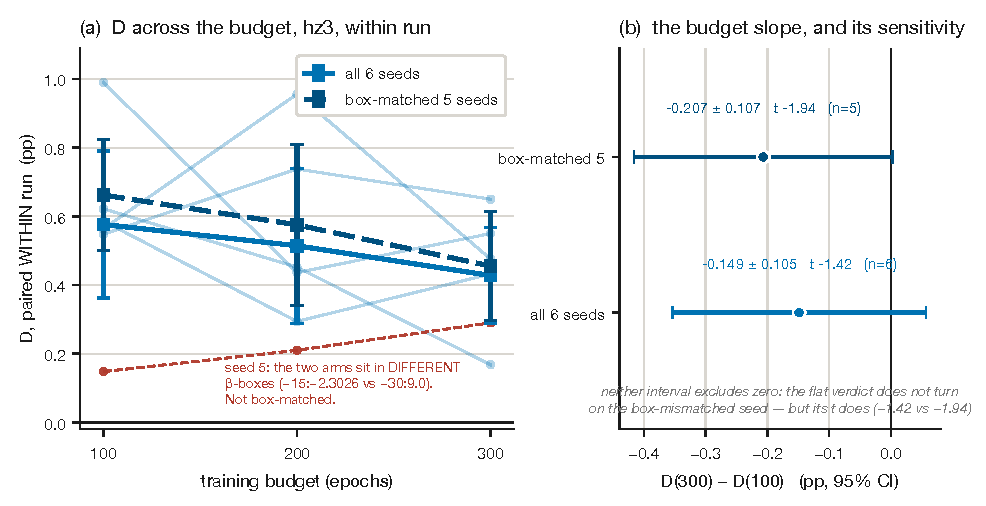
\includegraphics[width=\linewidth]{figures/f3_budget.pdf}
\caption{\textbf{$\Dstat$ at 1$\times$, 2$\times$ and 3$\times$ the budget, paired WITHIN run,
and what one box-mismatched seed did to it.} \arm{hz3} ran the four arms for 300 epochs at six
seeds, so $\Dstat$ can be read off the same run at three budgets, cancelling seed, run and batch
identically. (a) Faint blue lines are the archived per-seed trajectories; the heavy lines are
arm-set means with 95\% intervals. \textbf{Seed 5 is drawn in red because it is not box-matched}:
its chunk arm ran in $\beta$-box $-15{:}{-}2.3026$ and its \arm{nodewise} arm in $-30{:}9.0$, so
that seed's $\Dstat$ is a cross-box difference and the other five are not. The green dotted trace
is that same seed re-run box- and class-matched (\arm{hz3q}): \textbf{the archived reading rises
across the budget and the repaired one falls}, which is the whole of the repair. (b) The budget
slope, \textbf{all three readings together}, which is what the repair's own registered scorer
requires. It does not resolve on the six archived seeds ($-0.149 \pm 0.105$, $t\ -1.42$) or on the
five box-matched seeds alone ($-0.207 \pm 0.107$, $t\ -1.94$), and it does resolve, barely, on the
repaired pool ($\mathbf{-0.238 \pm 0.093}$, $t\ \mathbf{-2.57}$; \S\ref{sec:budget}). The archived
readings are kept in the panel rather than replaced by it, because the published record is part of
the evidence.}
\label{fig:budget}
\end{figure}

\section{Nine candidate mechanisms --- four refuted --- and two nulls}
\label{sec:mechanisms}

This section is the second half of the contribution, not an appendix. Of the nine, \textbf{four
are refuted} (M2, M3, M6, M9), \textbf{one is narrowed} to a base--meta pairing rather than to a
base alone (M4),
\textbf{one is not separable} from the axes it is aliased with (M7), and \textbf{three cannot be
decided by this instrument or this design} (M1 untested, M5 inapplicable, M8 not identifiable).
Two refutations rest on gates registered before their data existed (M2, M9); two are post-hoc
contrasts on data collected for other purposes (M3, M6). One further candidate, M1, had its
literature attribution withdrawn after we re-read the sources.

\textbf{M9 is the one refutation in this paper that was designed, registered, run and read in that
order.} Its bar --- \texttt{REFUTED if D >= +0.55} --- was committed in
\texttt{bin/c97\_sm4\_secondmoment.sh} before the batch was submitted, and it was cleared by a
wide margin in the direction the mechanism said was impossible. We report it as a positive result,
which is what it is.

\textbf{M7 is not a fourth refutation, and the reason is worth stating.} The contrast that would
make it one is a within-batch separator that the relevant batch's own registered scorer
\textbf{refuses to compute} (\S\ref{sec:level}, \S\ref{sec:threats} T7). Under
\S\ref{sec:registration} we report the refusal and not the contrast, so the refutation is
unavailable and M7 stands at \emph{not separable}. That is the most expensive single application
of \S\ref{sec:registration}'s rule in this
paper, and it is the reason the rule is worth stating as a contribution rather than as a habit.

\textbf{The refutations carry their own power limits and we print them with the verdicts.} M3 in
particular refuses a general \emph{size law} at $t\ 0.87$ and cannot rule out a tail-specific
effect; ``refuted'' there means the general form is refuted, not that the tail is exonerated
(\S\ref{sec:size1}). Table~\ref{tab:mechanisms} indexes all nine candidates, the verdict on each,
and the subsection that decides it.

\begin{table}[htbp]
\centering
\footnotesize
\caption{Index of the nine candidates, the verdict on each, and where each is decided.}
\label{tab:mechanisms}
\begin{tabular}{@{}cp{0.30\linewidth}p{0.42\linewidth}l@{}}
\toprule
\# & candidate mechanism & verdict & where \\
\midrule
M1 & $\sqrt{N}$ estimator-noise averaging over group members &
  \textbf{untested, not refuted} --- our instrument measures the wrong quantity; its literature
  attribution withdrawn & \S\ref{sec:sqrtn}, \S\ref{sec:rw-tensor} \\
M2 & Meta-gradient correlation (an $N_{\mathrm{eff}}/m$ field) predicts accuracy &
  \textbf{refuted} on its own pre-registered gate: anti-concordant $t\ -11.14$, dissociation
  $t\ -23.26$ & \S\ref{sec:field} \\
M3 & Degenerate size-1 groups are the carrier &
  \textbf{refuted} as a general size law: removing 100\% of singletons buys
  $+0.115 \pm 0.133$ ($t\ 0.87$) & \S\ref{sec:size1} \\
M4 & The size-1 tail carries it universally &
  \textbf{narrowed to a base--meta pairing, not to a base}: pooled
  $\Dstat - \Gstat = +0.514 \pm 0.056$ over the 8 CIFAR-10
  SGDm cells and $-0.061 \pm 0.085$ under AdamW\,+\,Lion (2 batches), but
  \textbf{$+0.629 \pm 0.242$ ($t\ 2.59$) under AdamW\,+\,RMSProp}. No individual $\Gstat$
  survives Holm on Welch df over the 14-test family & \S\ref{sec:tail},
  \S\ref{sec:normalisation} \\
M5 & Choi-style inclusion --- a finer partition contains the coarser one once tuned &
  \textbf{inapplicable}: granularity is state, not hyperparameters; the only setting where the
  arms coincide is $\eta = 0$ & \S\ref{sec:rw-choi}, \S\ref{sec:rule11} \\
M6 & The base optimiser's own second-moment normalisation &
  \textbf{refuted}: RMSProp and AdamW both carry one and differ by $+0.531 \pm 0.138$
  ($t\ 3.84$) on two-batch level pools & \S\ref{sec:normalisation} \\
M9 & A second-moment normaliser \textbf{anywhere in the loop} --- base or meta --- shrinks
  $\Dstat$ &
  \textbf{refuted on a pre-registered bar}: at the corner where both carry one,
  $\Dstat = +0.889 \pm 0.228$ ($t\ 3.89$), the \textbf{largest} $\Dstat$ in the AdamW family,
  against a registered refutation threshold of $\Dstat \ge +0.55$ & \S\ref{sec:normalisation} \\
M7 & $\Dstat$ tracks the aligned arm's accuracy level &
  \textbf{not separable}: the registered within-batch separator issued no verdict; the surviving
  slope is aliased with network and base optimiser ($-0.119 \pm 0.022$ holding base,
  $-0.386 \pm 0.105$ holding network, $-0.187 \pm 0.125$ holding both) & \S\ref{sec:level} \\
M8 & Some summary statistic of the group-size distribution &
  \textbf{not identifiable} from this design (rank 3, one contrast type) &
  \S\ref{sec:identifiability} \\
\bottomrule
\end{tabular}
\end{table}

\textbf{The two nulls}: architecture alignment (\S\ref{sec:alignment}, \S\ref{sec:null-repeat})
--- a \emph{bounded} null, $\Astat = -0.009 \pm 0.157$, 95\% CI $[-55\%, +51\%]$ of $\Dstat$,
replicated at $\Astat = -0.018 \pm 0.079$, 95\% CI $[-34\%, +28\%]$ of $\Dstat$ --- and
out-of-sample predictability of $\Dstat$
(\S\ref{sec:prediction}). \S\ref{sec:pooling} adds the failure of the classical remedy ---
hierarchical partial pooling --- which is a dead \emph{fix} rather than a dead mechanism, and is
included because CAM-HD makes it the obvious question to ask.

\subsection{Untested, not refuted: \texorpdfstring{$\sqrt{N}$}{sqrt(N)} estimator-noise averaging}
\label{sec:sqrtn}

The natural story is that a group of size $N$ averages $N$ meta-gradient samples, so a coarse
group's step-size estimate has noise $\propto 1/\sqrt{N}$ and fine partitions are noisier. We
built a per-group drift instrument to test it and got the wrong sign in every fit --- 6 of 6 ---
where a $1/\sqrt{N}$ model requires a log-log slope of $-0.500$. \emph{(That count is carried from
the project record and was \textbf{not} re-derived at write time; see
Appendix~\ref{app:discrepancy}.9. Nothing below rests on it.)}

\textbf{We do not present that as a refutation of the variance claim, because it is not one.} The
instrument measures \emph{drift} --- the per-step magnitude $|\Delta\bar{\beta}|$ --- which is net
systematic movement, not an estimator variance; and under Lion's sign update $|\Delta\beta| = \eta$
per step exactly, so the statistic is \textbf{censored at the meta-stepsize} (two published fits
ran through arms pinned at exactly $1.000\times10^{-3}$). The surviving fits are 4-point log-log
OLS with $R^2$ as low as 0.08. The only sentence this instrument supports is: \emph{the net drift
of a group's step-size exponent does not fall like $1/\sqrt{\text{group size}}$; we did not measure
the estimator variance.} The variance mechanism is \textbf{untested}, not refuted, and we say so.

Separately, and this is a correction to our own earlier writing: the attribution of a $\sqrt{N}$
noise-averaging argument to Adam-mini, Adalayer and SGG is \textbf{withdrawn}
(\S\ref{sec:rw-tensor}).

\subsection{Refuted: the meta-gradient correlation field predicts accuracy}
\label{sec:field}

A natural design principle for grouping is ``put weights with correlated meta-gradients
together'', which suggests an effective-sample-size statistic $N_{\mathrm{eff}}/m$ as a
predictor. We instrumented it and registered a five-way concordance test in advance. The
\arm{cc1} scorer, verbatim:

\begin{quote}\ttfamily\footnotesize
C2 \ aligned vs uniform at m=14,420\\
\ \ \ \ d\_acc = +0.727 pp (t +3.63, RESOLVED) \ \ d\_N\_eff/m = -0.0237 (t -11.14, RESOLVED)\\
\ \ \ \ -> **ANTI-CONCORDANT**\\
C3 \ aligned vs uniform at m=4,851, size-1 tail already gone\\
\ \ \ \ d\_acc = +0.011 pp (t +0.08, unresolved) \ d\_N\_eff/m = -0.0529 (t -23.26, RESOLVED)\\
\ \ \ \ -> **DISSOCIATION**\\
-> **MIXED: THE FIELD IS NOT A SUFFICIENT STATISTIC.**
\end{quote}

The negative is strong, not weak. The field channel resolves at $t\ -11$ and $t\ -23$ --- it is
not too noisy to read. It reads decisively, and decisively \emph{against} accuracy on one contrast
and silently on the other. This is the sharpest thing we can say to the meta-gradient-correlation
line of argument: the correlation statistic that line reaches for does not track the outcome it is
meant to justify.

\subsection{Refuted as a size law: size-1 groups are the carrier}
\label{sec:size1}

The most attractive explanation of \S\ref{sec:primary} is that $\Dstat$ is caused by the 9{,}610
degenerate size-1 groups in \arm{nodewise}. Inside one batch (\arm{ck1}) we removed \textbf{100\%
of a network's singletons} by going from one step size per weight (\arm{chunk1},
$m = 11{,}173{,}962$, 100\% singletons) to one per pair (\arm{chunk2}, $m = 5{,}586{,}981$,
\textbf{0\%} singletons):

\begin{quote}
\arm{chunk1} $90.979 \pm 0.131 \rightarrow$ \arm{chunk2} $91.095 \pm 0.024$. \textbf{Step
$= +0.115$, $\se$ 0.133, $t\ 0.87$ --- unresolved}, against a count-only prediction of $+0.13$ to
$+0.16$ from the family's own local secants.
\end{quote}

The ladder is smooth in $\log m$ with \textbf{no kink} at the one step where singleton fraction
collapses from 100\% to 0\%. Reported against our own interest, and \textbf{with its power
limit}: that step re-groups 100\% of 11.17M coordinates, whereas the tail in \arm{nodewise} is
0.086\% of the weights. It refuses a general \emph{size law}; it cannot rule out a tail-specific
effect. The unit is the \textbf{tensor}, not the group size.

\subsection{Narrowed to a base--meta pairing: the tail as a universal carrier}
\label{sec:tail}

$\Dstat - \Gstat$ (Eqs.~\ref{eq:D}--\ref{eq:G}) isolates the size-1 tail's contribution ---
$\Gstat$ is the same contrast with the tail already removed from both arms, count-matched
exactly. Table~\ref{tab:DG} gives the split cell by cell and Figure~\ref{fig:decomposition} plots
it, stacked in panel (a) and as the tail component alone in panel (b).

\begin{table}[htbp]
\centering
\small
\caption{The tail's contribution, cell by cell.}
\label{tab:DG}
\begin{tabular}{@{}lccrr@{}}
\toprule
cell & $\Dstat$ & $\Gstat$ & $\mathbf{\Dstat - \Gstat}$ & $t$ \\
\midrule
\arm{cc1} (SGDm) & $+0.727 \pm 0.200$ & $+0.011 \pm 0.147$ & $\mathbf{+0.715 \pm 0.248}$ & 2.88 \\
\arm{rl3} @$10^{-4}$ (SGDm) & $+0.681 \pm 0.173$ & $-0.011 \pm 0.087$ &
  $\mathbf{+0.692 \pm 0.194}$ & 3.57 \\
\arm{fa1} (SGDm) & $+0.629 \pm 0.123$ & $-0.001 \pm 0.076$ & $\mathbf{+0.630 \pm 0.145}$ & 4.35 \\
\arm{hz3} (SGDm, 300 ep) & $+0.428 \pm 0.086$ & $-0.057 \pm 0.061$ &
  $\mathbf{+0.484 \pm 0.106}$ & 4.57 \\
\arm{g3m} (SGDm, R34) & $+0.666 \pm 0.094$ & $+0.171 \pm 0.073$ & $\mathbf{+0.495 \pm 0.119}$ &
  4.15 \\
\arm{r50} (SGDm, R50) & $+0.881 \pm 0.261$ & $+0.153 \pm 0.314$ & $\mathbf{+0.729 \pm 0.409}$ &
  1.78 \\
\arm{gm2} (SGDm, C100) & $+1.485 \pm 0.238$ & $+0.068 \pm 0.069$ & $\mathbf{+1.417 \pm 0.248}$ &
  5.72 \\
\arm{nl1} (RMSProp) & $+0.973 \pm 0.251$ & $+0.020 \pm 0.049$ & $\mathbf{+0.953 \pm 0.256}$ &
  3.72 \\
\arm{ml2} (SGDm) & $+0.456 \pm 0.195$ & $+0.173 \pm 0.073$ & $\mathbf{+0.282 \pm 0.208}$ & 1.36 \\
\arm{rl3} @$3{\times}10^{-4}$ (SGDm) & $+0.591 \pm 0.096$ & $+0.217 \pm 0.128$ &
  $\mathbf{+0.375 \pm 0.160}$ & 2.34 \\
\arm{nl1} (SGD) & $+1.035 \pm 0.109$ & $+0.525 \pm 0.294$ & $\mathbf{+0.510 \pm 0.314}$ & 1.63 \\
\textbf{\arm{aw1} (AdamW + Lion)} & $+0.279 \pm 0.087$ & $\mathbf{+0.232 \pm 0.089}$ &
  $\mathbf{+0.047 \pm 0.124}$ & \textbf{0.38} \\
\textbf{\arm{sm3} (AdamW + Lion)} & $+0.141 \pm 0.064$ & $\mathbf{+0.296 \pm 0.096}$ &
  $\mathbf{-0.155 \pm 0.116}$ & $\mathbf{-1.34}$ \\
\textbf{\arm{sm4} (AdamW + RMSProp)} & $+0.889 \pm 0.228$ & $\mathbf{+0.261 \pm 0.081}$ &
  $\mathbf{+0.629 \pm 0.242}$ & \textbf{2.59} \\
\bottomrule
\end{tabular}
\end{table}

\arm{ml2}'s three standard errors are computed on \textbf{three} independent seeds, not six runs:
its two nominal halves are the same command line including \texttt{--seed}, so the batch is three
seeds run twice rather than six seeds (\S\ref{sec:silent-failures}). Averaging within seed before
differencing gives $\Dstat +0.456 \pm 0.195$ ($t\ 2.34$), $\Gstat +0.173 \pm 0.073$ ($t\ 2.38$),
$\Dstat - \Gstat +0.282 \pm 0.208$ ($t\ 1.36$). \textbf{Every point estimate is unchanged}; only
the standard errors move. \arm{hz3} matched at 5 v 5 for the seed-5 mismatch of
\S\ref{sec:threats} T9 reads $\Dstat +0.455 \pm 0.096$, $\Gstat -0.050 \pm 0.075$,
$\Dstat - \Gstat +0.506 \pm 0.121$, $t\ 4.16$ --- same verdict; and repaired at 6 v 6 with
\arm{hz3q}'s seed 5, $\Dstat +0.394 \pm 0.093$, $\Gstat -0.048 \pm 0.061$,
$\Dstat - \Gstat +0.442$ --- same verdict again.

\paragraph{The $\Gstat$ tests, corrected for multiplicity.}
$\Gstat$ is measured once per count-matched cell, so the values above are a family and the
ones that reach nominal significance should not be read one at a time. We declared the family as
the $\Gstat$ leg of every Table~\ref{tab:D} cell that has one --- twelve tests, fixed before the
correction was computed --- and applied Holm--Bonferroni step-down \citep{holm1979simple} at
$\alpha = 0.05$. \textbf{Table~\ref{tab:D} has since grown by four cells, two of which have a
$\Gstat$} (\arm{sm3} and \arm{sm4}; \arm{bm2} ran only \arm{nodewise} and \arm{chunk777}, and its
registered scorer forbids any $\Gstat$ or tail statement from it), so the same rule now yields
\textbf{fourteen} tests. We report the pre-specified twelve first, unchanged, and then the
fourteen, so that the effect of enlarging the family is visible rather than absorbed
(Table~\ref{tab:holm}). Each $p$ is the two-sided Welch test on the two arm means; $p\ (z)$ is the normal
approximation, which is the quantity the paper's $t$ columns report and is anti-conservative at
2--4 degrees of freedom. Each Holm column is computed on its own ordering.

\begin{table}[htbp]
\centering
\small
\caption{The twelve-test $\Gstat$ family under Holm--Bonferroni. At most three reach nominal
$\alpha = 0.05$ and none survives Holm in either convention.}
\label{tab:holm}
\begin{tabular}{@{}lrrrrrrrr@{}}
\toprule
cell & $\Gstat$ & $\se$ & $t$ & df & $p$ (Welch) & $p$ Holm & $p$ ($z$) & $p$ Holm ($z$) \\
\midrule
\arm{g3m} (SGDm, R34)   & $+0.171$ & 0.073 & 2.34 & 16.0 & \textbf{0.033} & 0.39 & 0.0195 & 0.20 \\
\arm{aw1} (AdamW)       & $+0.232$ & 0.089 & 2.62 & 3.5 & 0.067 & 0.74 & 0.0089 & 0.11 \\
\arm{ml2} (SGDm)        & $+0.173$ & 0.073 & 2.38 & 4.0 & 0.076 & 0.76 & 0.0171 & 0.19 \\
\arm{rl3} @$3{\times}10^{-4}$ & $+0.217$ & 0.128 & 1.69 & 3.9 & 0.168 & 1.00 & 0.091 & 0.73 \\
\arm{nl1} (SGD)         & $+0.525$ & 0.294 & 1.79 & 2.8 & 0.177 & 1.00 & 0.074 & 0.67 \\
\arm{gm2} (SGDm, C100)  & $+0.068$ & 0.069 & 0.99 & 3.5 & 0.386 & 1.00 & 0.322 & 1.00 \\
\arm{hz3} (SGDm, 300 ep)& $-0.057$ & 0.061 & $-0.93$ & 6.2 & 0.389 & 1.00 & 0.354 & 1.00 \\
\arm{r50} (SGDm, R50)   & $+0.153$ & 0.314 & 0.49 & 3.9 & 0.653 & 1.00 & 0.627 & 1.00 \\
\arm{nl1} (RMSProp)     & $+0.020$ & 0.049 & 0.41 & 3.4 & 0.710 & 1.00 & 0.686 & 1.00 \\
\arm{rl3} @$10^{-4}$    & $-0.011$ & 0.087 & $-0.12$ & 2.1 & 0.913 & 1.00 & 0.902 & 1.00 \\
\arm{cc1} (SGDm)        & $+0.011$ & 0.147 & 0.08 & 2.4 & 0.944 & 1.00 & 0.938 & 1.00 \\
\arm{fa1} (SGDm)        & $-0.001$ & 0.076 & $-0.01$ & 9.8 & 0.993 & 1.00 & 0.993 & 1.00 \\
\bottomrule
\end{tabular}
\end{table}

\textbf{At most three of the pre-specified twelve reach nominal $\alpha = 0.05$ and none survives
Holm.} On the
normal approximation the three are \arm{aw1} ($t\ 2.62$), \arm{ml2} ($t\ 2.38$) and \arm{g3m}
($t\ 2.34$), with smallest adjusted $p = 0.11$; on the Welch degrees of freedom only \arm{g3m}
reaches nominal $\alpha$, with smallest adjusted $p = 0.39$.

\textbf{On the family of fourteen, the Welch verdict is unchanged and the normal-approximation
verdict is not.} Adding \arm{sm3} ($\Gstat = +0.296 \pm 0.096$, $t\ 3.07$, Welch df 3.5) and
\arm{sm4} ($\Gstat = +0.261 \pm 0.081$, $t\ 3.23$, Welch df 3.7): on Welch degrees of freedom
\textbf{nothing survives Holm} (smallest adjusted $p = 0.46$, \arm{g3m}); on the
anti-conservative normal approximation \textbf{\arm{sm4} (adjusted $p = 0.017$) and \arm{sm3}
(adjusted $p = 0.028$) both survive}, which no tabled cell did at twelve. We record that without
resting anything on it, because the normal approximation is the wrong reference at 3.5 degrees of
freedom and we say so elsewhere in this paper. The enlarged family carries more raw heterogeneity than
the pre-specified one --- fourteen-cell $\Gstat$ pool $+0.093 \pm 0.022$, $Q = 28.25$ on 13 df,
against the twelve-cell $+0.067 \pm 0.023$, $Q = 18.21$ on 11 df --- and the two cells that make
it so are the two new AdamW-base ones. \textbf{Neither $Q$ resolves, and an earlier version of
this paragraph, which read the fourteen as heterogeneous where the twelve was not, rested on the
wrong reference and is corrected here.} Those two $\chi^2$ $p$-values are 0.0084 and 0.077;
simulating this family's own null exactly as \S\ref{sec:threats} T13 simulates
\S\ref{sec:moderator}'s --- same cells, same arms, the same \texttt{welch()} and
\texttt{meta()}, 20{,}000 draws at the registered seed --- gives a null $Q$ with mean 24.0 on
13 df and 20.1 on 11 df, and \textbf{Monte-Carlo $p$ 0.26 and 0.42}. The contrast between the
two families is a property of the reference, not of the cells.

\textbf{We therefore make no claim
that $\Gstat$ is resolved in any individual cell}, and an earlier version of this section, which
rested on $\Gstat$ being resolved under AdamW, is withdrawn as a per-cell claim.

What survives the correction is not a cell but a \textbf{contrast between base optimisers}, which
is a single pre-specified comparison and needs no family correction: $\Dstat - \Gstat$ is
$+0.047 \pm 0.124$ ($t\ 0.38$) under AdamW against a fixed-effect pool of
$\mathbf{+0.514 \pm 0.056}$ ($t\ 9.2$) over the eight CIFAR-10 SGDm cells ($Q\ 4.52$ on 7 df;
restricted to the six ResNet-18/CIFAR-10 cells it is $+0.514 \pm 0.064$, the same point estimate).
Adding the CIFAR-100 cell would give $+0.558 \pm 0.055$ with $Q\ 17.17$ on 8 df, which
\S\ref{sec:primary}'s commensurability rule forbids and which is that rule doing measurable work
rather than being a stylistic preference. The tail accounts for essentially none of $\Dstat$ under
AdamW and for essentially all of it under SGDm, and that difference --- not any single $\Gstat$
--- is the result.

The independent AdamW measurement is \arm{sm3}, and its runs \textbf{are} now in the deposited run
table, so it enters the table above rather than sitting beside it: $\Gstat = +0.296 \pm 0.096$,
$\Dstat - \Gstat = -0.155 \pm 0.116$
at the same cell as \arm{aw1} (\S\ref{sec:silent-failures}). The two AdamW\,+\,Lion batches pool
to $\mathbf{\Dstat - \Gstat = -0.061 \pm 0.085}$ ($Q$ 1.41 on 1 df); on the 6 v 6 concatenation of
their seeds the same quantity reads $-0.054 \pm 0.082$ ($t\ -0.66$). Under an AdamW base with a
Lion meta-optimiser, the size-1 tail contributes nothing measurable to $\Dstat$, and that now
rests on two independent submissions rather than one.

\textbf{One $\Gstat$ contrast exists in the corpus outside this table}, and we name it so the
family is auditable rather than convenient. \arm{bn1} ran \arm{nodewise1d} and \arm{chunk2325}
($m = 4{,}851$ in both arms) but no \arm{chunk777} arm, so it yields a $\Gstat$ and no $\Dstat$:
$\Gstat = +0.295 \pm 0.048$, the largest $\Gstat$ in the corpus and the only large positive
$\Gstat$ under an SGDm base --- which cuts against ``under SGDm, removing the tail removes the
gap''. (\arm{sm3}'s $\Gstat$, which an earlier version of this section also listed here, is now a
tabled cell.) Enlarging the family to all fifteen and
re-running Holm changes the count but not the verdict on Welch degrees
of freedom, where \textbf{nothing survives}; on the normal approximation
\arm{bn1} (adjusted $p = 1.2\times10^{-8}$), \arm{sm4} (0.017) and \arm{sm3} (0.028) survive.
The fifteen-test family carries the largest $\Gstat$-layer $Q$ in the paper ($\Gstat$ pool
$+0.128 \pm 0.020$, $Q = 42.98$ on 14 df), and \textbf{it does not resolve either}: $\chi^2_{14}$
puts it at $p = 8.6\times10^{-5}$, its own simulated null (mean 26.1, \S\ref{sec:threats} T13)
at \textbf{Monte-Carlo $p$ 0.12}. An earlier version of this sentence called the family
heterogeneous on the $\chi^2$ reading alone. What is visible without a $p$ is that the $Q$ is
driven
by \arm{bn1}; \arm{bn1} and \arm{cc1} are the same configuration in different batches and their
$\Gstat$ values differ by $0.284 \pm 0.155$ ($t\ 1.83$), i.e.\ not resolved, which is what
\S\ref{sec:variance}'s cross-batch bound predicts. We disclose it rather than leave a referee to
find it.

Under SGDm, removing the tail removes the gap. \textbf{Under AdamW with a Lion meta it does not}:
$\Dstat - \Gstat$ is $+0.047 \pm 0.124$ in \arm{aw1} and $-0.155 \pm 0.116$ in \arm{sm3}, pooling
to $-0.061 \pm 0.085$, against $+0.514 \pm 0.056$ pooled
over the eight CIFAR-10 SGDm cells. $\Gstat$ itself is positive under AdamW
($+0.232 \pm 0.089$ and $+0.296 \pm 0.096$) but survives Holm over the $\Gstat$ family on Welch
degrees of freedom in neither cell, so the
dependence is carried by the $\Dstat - \Gstat$ contrast, which is one pre-specified
comparison, not by a per-cell $\Gstat$ verdict.

\paragraph{The dependence is not on the base optimiser alone, and this is new.}
Holding the base at AdamW and everything else at \arm{aw1}'s cell, and changing only the
meta-optimiser from Lion to RMSProp:

\begin{center}
\small
\begin{tabular}{@{}lccc@{}}
\toprule
statistic & AdamW + Lion (\arm{aw1}, \arm{sm3}) & AdamW + RMSProp (\arm{sm4}) & difference \\
\midrule
$\Dstat$ & $+0.189 \pm 0.052$ & $\mathbf{+0.889 \pm 0.228}$ & $\mathbf{+0.700 \pm 0.234}$ \\
$\Gstat$ & $+0.261 \pm 0.065$ & $\mathbf{+0.261 \pm 0.081}$ & $\mathbf{-0.001 \pm 0.104}$ \\
$\Dstat - \Gstat$ & $-0.061 \pm 0.085$ & $\mathbf{+0.629 \pm 0.242}$ &
  $\mathbf{+0.690 \pm 0.257}$ \\
\bottomrule
\end{tabular}
\end{center}

\textbf{$\Gstat$ does not move at all --- the two readings agree to a thousandth of a percentage
point --- and the whole of the meta-optimiser's effect on $\Dstat$ lands in the size-1 tail
component.} The \arm{sm4} scorer reaches the same two conclusions independently and states them as
its own registered verdicts: \texttt{G PERSISTS. The exactly count-matched contrast stays resolved
when the meta also carries a second moment, as it is under AdamW+Lion (aw1 +0.232, sm3 +0.296). G
is base-dependent, not meta-dependent, at this corner.} And on the mechanism contrast:
\texttt{MECHANISM CONTRAST RESOLVED at |t| >= 2 (interval [+0.154, +1.104]). Under AdamW+Lion it
is NOT resolved in either batch (aw1 +0.047, sm3 -0.155), so a resolved D-G here is a finding
about the meta-optimiser.}

\paragraph{What that costs the tail story.}
M4 was narrowed in the previous version of this paper to ``an SGDm base with a Lion meta-optimiser'', with AdamW
as the counter-example. The counter-example does not survive as a statement about the base: at an
AdamW base the tail carries nothing under Lion and carries $+0.629 \pm 0.242$ under RMSProp.
\textbf{The tail's contribution is a property of the base--meta pairing, not of the base}, and
this corpus has measured only two of the four pairings it would take to say which side dominates
--- it has no SGDm\,+\,RMSProp cell at all. The two right-hand columns of the table above are
\textbf{cross-batch} comparisons and carry the cross-batch offset this paper measures elsewhere
--- bounded at about 0.32 pp at matched science and not separable from within-arm noise
(\S\ref{sec:variance}); the $F(62,85) = 5.47$ this sentence used to cite is withdrawn and does not
re-derive (Appendix~\ref{app:discrepancy}.3) --- which neither pairing nor Welch removes; they are
labelled comparisons, not registered tests, and the \arm{sm4} registration explicitly forbids
pooling \arm{sm4} with \arm{aw1} or \arm{sm3}. What is a registered test is \arm{sm4}'s own
within-batch $\Dstat - \Gstat = +0.629 \pm 0.242$ ($t\ 2.59$), and it is resolved. The pre-registration for that batch said, before
the data existed, that \emph{``a RESOLVED non-null G would say the tail story is base-dependent
and must be re-scoped.''} The re-scoping is warranted on the contrast; the word ``resolved'' is
not, and we do not use it.

\begin{quote}
\textbf{``The gap lives in the degenerate size-1 tail'' may not be written as a general claim, and
may not be scoped to a base optimiser either.} It holds under an SGDm base with a Lion
meta-optimiser (eight cells, seven submissions) and under an AdamW base with an RMSProp meta (one
cell); it fails under an AdamW base with a Lion meta (two cells). The scoping variable is the
pairing, and three of its four cells are one batch each.
\end{quote}

The same batch's $\Dstat$ itself is \textbf{UNRESOLVED} on its own registered rule:
\texttt{analysis/c88\_scorers.py --score aw1} prints

\begin{quote}\ttfamily\footnotesize
\{'D\_adamw': 0.279, 'se': 0.087, 't': 3.19,\\
\ 'rule': "UNRESOLVED at n=6. Report the interval. Do NOT re-cut the\\
\ \ data, and do NOT describe it as 'partially transferring'."\}
\end{quote}

\noindent The registered bar was a 95\% lower bound above $+0.30$; the realised bound is $\mathbf{+0.108}$
(normal approximation; $\mathbf{+0.038}$ on Welch df 4), so the bar is not cleared. The
registration also specified 6 seeds where only 3 reached the contrast, so the primary ran at half
its registered power --- a registration deviation disclosed again, with its cause, in
\S\ref{sec:repro}. \textbf{$\Dstat$ under AdamW is reported as an interval,
$+0.279\ [0.108, 0.450]$, not as a transfer.}

\begin{figure}[htbp]
\centering
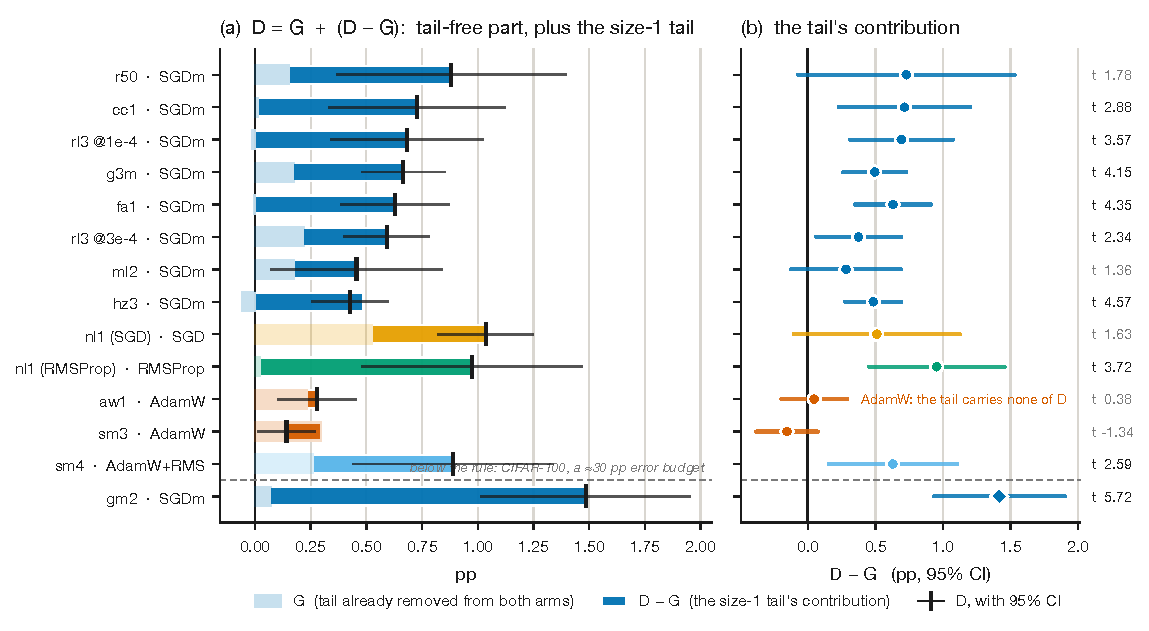
\includegraphics[width=\linewidth]{figures/f4_decomposition.pdf}
\caption{\textbf{$\Dstat$ splits into a tail-free part $\Gstat$ and a size-1-tail part
$\Dstat - \Gstat$, and the split depends on the base--meta pairing.} (a) For every batch that ran
all four arms,
$\Dstat$ is drawn as the sum of $\Gstat$ (hatched: the same uniform-versus-aligned contrast with
the size-1 tail \emph{already removed from both arms}, count-matched exactly at $m = 4{,}851$) and
$\Dstat - \Gstat$ (solid: what the tail contributes). The black tick and whisker are $\Dstat$
itself with its 95\% interval. Under an SGDm base with a Lion meta the hatched part is
$\approx 0$ and the tail
carries essentially all of $\Dstat$. Under \textbf{AdamW with a Lion meta} it does not: $\Gstat$
is $+0.232 \pm 0.089$ (\arm{aw1}) and $+0.296 \pm 0.096$ (\arm{sm3}) while $\Dstat - \Gstat$ is
$+0.047 \pm 0.124$ and $-0.155 \pm 0.116$, pooling to $-0.061 \pm 0.085$. Under \textbf{AdamW with
an RMSProp meta} (\arm{sm4}, the only non-Lion cell in the corpus) $\Gstat$ is unchanged at
$+0.261 \pm 0.081$ while $\Dstat - \Gstat$ returns to $+0.629 \pm 0.242$ ($t\ 2.59$) --- $\Gstat$
does not move with the meta-optimiser and the tail component does. (b) $\Dstat - \Gstat$
alone, with 95\% intervals and each cell's $t$. CIFAR-100 is placed below the rule for the reason
given in Figure~\ref{fig:forest}. The pooled SGDm/CIFAR-10 value is $\mathbf{+0.514 \pm 0.056}$
over eight cells ($Q\ 4.52$ on 7 df); we quote that pool rather than \arm{cc1}'s $+0.715$, which
is the maximum.}
\label{fig:decomposition}
\end{figure}

\subsection{Refuted twice: second-moment normalisation, in the base (M6) and in the meta (M9)}
\label{sec:normalisation}

\paragraph{M6, the base side, post-hoc.}
If the mechanism were ``a base optimiser that already normalises per coordinate does not need the
partition to do it'', then RMSProp and AdamW --- both carrying a second moment --- should behave
alike. They do not. On the two-batch level pools of \S\ref{sec:moderator},
$\mathbf{\Dstat(\text{RMSProp}) - \Dstat(\text{AdamW}) = +0.531 \pm 0.138}$, $t\ 3.84$; on the
single-batch reading the previous version of this paper quoted, the independent \arm{nl1}-versus-\arm{aw1}
contrast, it was $+0.694 \pm 0.266$, $t\ 2.61$. The refutation is the same and it is now carried
by four batches instead of two. It remains a \textbf{post-hoc contrast} on data collected for
other purposes, and the AdamW half of it comes entirely from \arm{aw1} and \arm{sm3}: \arm{bm2}'s
registered scorer forbids \arm{bm2} any statement about AdamW, and none is made.

\paragraph{M9, the meta side, pre-registered.}
M6 leaves the strongest form of the normalisation story standing. Every base-side comparison in
this corpus varies the base while a \textbf{Lion} meta-optimiser sits above it, and Lion's sign
update carries no second moment at all. So the claim ``$\Dstat$ shrinks wherever a second-moment
normaliser sits, base \textbf{or} meta'' had never been tested at the one corner that decides it:
an AdamW base with an RMSProp meta, where both components carry one. That corner predicts the
\emph{smallest} $\Dstat$ in the corpus. \arm{sm3} was built to run it and did not --- its own
\texttt{ARGS:} line carries \texttt{--alg-meta} twice and argparse kept the last occurrence, so it
ran Lion (\S\ref{sec:silent-failures}). The corner was therefore untested, not refuted, and it
stayed that way for a full cycle.

\arm{sm4} runs it. Four granularity arms $\times$ three seeds at \arm{aw1}'s own cell ---
ResNet-18/CIFAR-10, $\alpha_0 = 10^{-3}$, $\eta = 10^{-4}$, box $-15{:}{-}2.3026$, 100 epochs,
\texttt{AUGMENT=1} --- changing exactly one flag, \texttt{--alg-meta Lion} $\rightarrow$
\texttt{--alg-meta RMSProp}, with RMSProp's own attribute set live and Lion's two attributes set
to the code's $-1$ sentinel so they are dropped before the optimiser is built. The decision rule
was frozen in the batch script before submission, and we quote it from the script rather than
paraphrasing it:

\begin{quote}\ttfamily\footnotesize
Mechanism candidate 8 says D shrinks wherever a second-moment normaliser sits. […] This corner
carries a second moment on BOTH sides, so the pattern predicts the SMALLEST D in the corpus.\\
\ \ REFUTED if D >= +0.55.\\
CONSISTENT if D <= +0.279 (aw1's own D) with a 95\% interval below the bar.\\
UNDECIDED otherwise -- report the interval, add no seeds to this batch, and re-register a fresh
replicate instead. All three outcomes are publishable and the scorer prints the one that fires;
nothing here is chosen after the fact.
\end{quote}

Three gates fire before the contrast. The ARGS gate (RULE 20) read all twelve runs' own
\texttt{ARGS:} lines: \texttt{CLEAN --- every run's own ARGS line matches the declared design, no
repeated flag, no Lion attribute live} --- which is the check \arm{sm3} would have failed. The box
gate, measured on \arm{sm4}'s own probe records, reports \texttt{coord\_lo} and \texttt{coord\_hi}
of exactly 0.00000 on all four arms. And an operating-point gate, blocking and registered in
advance because no RMSProp meta-optimiser had ever run anywhere in this corpus and its
meta-stepsize was matched to \arm{aw1} rather than tuned: \texttt{ON ANCHOR. 12-run mean plateau5
91.567 against the AdamW+Lion anchor 93.161 (-1.594 pp, bar 3.0). The cell is comparable.} Had it
fired, every contrast in the batch would have been demoted to descriptive and labelled off-anchor
--- reported, not discarded.

The verdict, from \texttt{analysis/c97\_sm4\_score.py} run unedited:

\begin{quote}\ttfamily\footnotesize
D = chunk777 - nodewise = +0.8893 +- 0.2285~~~t +3.89 (df 2.3, p 0.0494)~~~n 3v3\\
95\% CI [+0.4415, +1.3371]\\
VERDICT: REFUTED. D >= +0.55 at the corner where BOTH the base and the meta carry a second-moment
normaliser. Mechanism candidate 8 -- 'D shrinks wherever a second moment sits' -- is false, and
the AdamW/RMSProp pattern in the corpus needs another explanation. This is a POSITIVE result and
must be reported as one, not buried.
\end{quote}

\textbf{The corner that predicted the smallest $\Dstat$ in the corpus produced the largest
$\Dstat$ in the AdamW family}: $+0.889$ against \arm{aw1}'s $+0.279$, \arm{sm3}'s $+0.141$, and
their pool of $+0.189 \pm 0.052$ --- a between-batch difference of $+0.700 \pm 0.234$. Whatever
the AdamW-versus-RMSProp pattern in \S\ref{sec:moderator} is, it is not a count of second-moment
normalisers in the loop.

\paragraph{Scope, carried with the verdict because the scorer carries it.}
The batch runs at \arm{aw1}'s meta-stepsize of $10^{-4}$, \textbf{not at an RMSProp-meta optimum}
--- no meta-stepsize ladder exists under an RMSProp meta, because this corpus contains no other
RMSProp-meta run of any kind. It is ResNet-18 / CIFAR-10 / 100 epochs / box $-15{:}{-}2.3026$
only. And it is \textbf{not pooled with \arm{aw1} or \arm{sm3}}: different meta-optimiser,
different batch. One cell refutes a claim that was stated over the whole grid; it does not
establish anything about the RMSProp-meta cell that a ladder would.

\paragraph{What this does to \S\ref{sec:moderator}'s $2 \times 2$.}
The previous version of this paper read the four-level base decomposition as agreeing with M6 about which
component of the base optimiser is not the axis, on the strength of an unresolved second-moment
main effect ($-0.169 \pm 0.145$, $z\ -1.16$). On the fourteen-cell pools that main effect resolves
($-0.323 \pm 0.080$, $z\ -4.03$) and the agreement is gone. \textbf{We withdraw the claim that the
two analyses agree.} What both still support is the weaker and more useful statement: neither
momentum nor second-moment normalisation, taken alone, is the moderator --- the momentum collapse
leaves a residual $Q$ of 34.64 on 9 df --- and M9 shows that adding a second moment to the
\emph{meta}-optimiser moves $\Dstat$ in the direction opposite to the one the normalisation story
requires.

\subsection{Not dead, not separable: \texorpdfstring{$\Dstat$}{D} and the aligned arm's accuracy
level}
\label{sec:level}

Over all 10 design points (\S\ref{sec:prediction} states the grouping rule), regressing $\Dstat$
on the aligned arm's \plateau{} gives slope $\mathbf{-0.045 \pm 0.011}$, $t\ -4.21$, $r\ -0.830$
--- which looks like a law and is not one, because level and dataset are the same column: the
single CIFAR-100 design point sits at level 70.44 and the nine CIFAR-10 design points at
89.63--93.04.

Inside CIFAR-10 the slope is $\mathbf{-0.176 \pm 0.056}$, $t\ -3.16$, $r\ -0.767$ over 9 design
points (exact permutation over all $9! = 362{,}880$ orderings, $p = 0.0151$). \textbf{This is
a strengthening we did not want and report anyway}: on the sixteen-cell set, grouped by the same
rule, the same regression read $-0.162 \pm 0.074$, $r\ 0.666$ against a critical 0.707 at eight
points --- unresolved, and the previous version of this paper, which split two cells that this
rule joins and so read the sixteen cells at nine CIFAR-10 points, got $r\ 0.669$ against a
critical 0.666 and called it a coin landing on its edge. Ingesting \arm{bm2}, \arm{sm3} and \arm{sm4} merges three pairs of cells
into their design points, which reduces measurement error in \emph{both} columns and de-attenuates
the slope. So the association is now resolved, and the three things that stop it being a mechanism
are the ones that matter.

\begin{itemize}
\item \textbf{It is aliased with the network and with the base optimiser, and the alias is the
  whole effect.} The two lowest-level CIFAR-10 design points are \arm{r50} (a different network)
  and \arm{sm4} (a different meta-optimiser), with \arm{nl1}/\arm{bm2}/SGD next. Holding the base
  fixed at SGDm (5 points, spanning ResNet-18/34/50) gives $\mathbf{-0.126 \pm 0.022}$; holding
  the network fixed at ResNet-18 (7 points, spanning five base--meta pairings) gives
  $\mathbf{-0.287 \pm 0.075}$; holding \textbf{both} fixed --- the only three points where
  ``level'' varies with nothing else structural --- gives $\mathbf{-0.188 \pm 0.148}$,
  $t\ -1.27$, \textbf{unresolved}. At three points the exact permutation test carries no
  information: its smallest attainable two-sided $p$ is $2/3! = 0.333$ and the observed slope
  reaches only $p = 0.667$, so the $t$ is the only reading available. It is also the reading that
  matters. A slope whose magnitude moves by $2.3\times$ depending on which confound you hold, and
  which does not resolve when you hold both, is measuring the confounds.
\item \textbf{An instrument that does not share an arm with $\Dstat$ does not settle it either.}
  $\Dstat$ and level share the \arm{nodewise} arm. The mechanical slope this induces is
  $\mathbf{-0.014}$ --- the mean sampling variance of a \arm{nodewise} arm mean over the 18
  CIFAR-10 cells, 0.01724, over the variance of level across the nine design points, 1.19374 ---
  under a tenth of $-0.176$, so the artefact is not the explanation. (An earlier version of this paper printed
  0.01808 for the first of those two inputs; that value does not re-derive under either a
  cell-level or a point-level average and is replaced rather than restated.) Replacing level by an
  independent instrument --- the mean of the \arm{chunk2325} and \arm{nodewise1d} arms, neither of
  which enters $\Dstat$ --- gives $\mathbf{-0.208 \pm 0.089}$, $t\ -2.33$ within CIFAR-10, which
  now clears $|t| \ge 2$ where the sixteen-cell reading ($-0.168 \pm 0.112$, $t\ -1.50$) did not.
  The association is therefore not an arm-sharing artefact; it is still not separable from the
  network and the base.
\item \textbf{The one within-batch contrast left in the corpus does not resolve it either.}
  \arm{rl3} ran both meta-stepsize rungs in one batch: level moves $+0.599$ pp
  ($91.908 \rightarrow 92.507$) and $\Dstat$ moves $-0.090$ ($+0.681 \rightarrow +0.591$), an
  implied within-batch slope of $\mathbf{-0.150 \pm 0.331}$ ($t\ -0.45$). Same sign as the
  between-point slope, and an interval that contains zero and all three sub-slopes above. It is
  also confounded with $\eta$, which is why it is a consistency check and not a test.
\end{itemize}

\textbf{The registered within-batch separator issued no verdict.} \arm{gn1} was built to answer
exactly this question --- one batch, one variable changed (BatchNorm $\rightarrow$ GroupNorm),
batch cancels --- and its pre-registered commensurability gate fired: the two halves sit on error
budgets of 7.707 pp and 10.569 pp, a $1.37\times$ ratio against a registered bar of 2.0 pp, so a
percentage-point contrast between them is not defined. Its scorer prints \textbf{``NO TRANSFER
VERDICT IS ISSUED \ldots{} THIS IS NOT A NULL''} and halts before computing either contrast. An
earlier version of this paper quoted that batch's face values as a falsification of the level
model --- a within-batch \texttt{dD} of $-0.385 \pm 0.205$, described as wrong-signed by 2.2 to
7.0 $\se$. We withdraw that, and we withdraw the falsification with it. \textbf{Both legs of the
earlier argument came from the withdrawn cell}: it was the within-batch test, and it was also the
low-level point that flattened the within-CIFAR-10 slope, which without it moves from
$-0.045 \pm 0.076$ ($t\ -0.59$) to the $-0.176 \pm 0.056$ above. The paper is weaker here than the
previous version of this paper claimed, and in the direction the level model predicts.

\textbf{What is left is an honest negative-space statement, not a dead mechanism.} The accuracy
level of the aligned arm is not separable from the network and the base optimiser in this corpus,
at 9 CIFAR-10 design points, where it is resolved ($|r|$ 0.767 against a critical 0.666) and
still collapses to $t\ -1.27$ the moment the network and the base are both held fixed. We do not
claim it is a carrier; we do
not claim it is not; and \S\ref{sec:prediction} shows that as a \emph{predictor} it is the worst
of the four models we tried, out of sample. The design needed to separate it --- a level contrast
at fixed network, fixed base and commensurable error budget --- is stated in
\S\ref{sec:conclusion}.

\subsection{Not identifiable (and un-killable): a summary statistic of the size distribution}
\label{sec:identifiability}

We constructed exact group-size multisets for every (network, granularity) cell we could
instantiate --- 150 of 163 attempted, the rest being block partitions applied to the wrong network
depth, which the optimiser rejects --- by instantiating the optimiser on CPU and reading sizes off
its own allocated state, with two receipts asserted on every cell
($\sum \text{size} \times \text{count} = \sum p.\texttt{numel()}$;
$\sum \text{count} = \texttt{beta}$ elements allocated) passing on all 150, and reproducing every
group count in this paper exactly. We then scored twenty candidate statistics ---
mean/median/sd/CV/skew/min/max, harmonic and geometric mean, sd of log size, categorical and
weighted entropy, inverse participation ratio, Gini, singleton fractions by group and by weight,
threshold fractions, and a heterogeneity index.

An earlier analysis nominated the degeneracy indicator with an apparently decisive fit.
\textbf{That positive claim is deleted, and the reason it is deleted is the finding.}
\texttt{frac\_groups\_size1} takes exactly \textbf{two values} across the entire count-matched
design --- 0.6664 on \arm{nodewise}, 0.0000 on all three other arms, on every network. Re-running
the analyst's own shape test with (a) that statistic, (b) a bare 1/0 ``is this arm
\arm{nodewise}'' dummy, (c) an arbitrary two-level regressor, and (d) the plain test that the
three non-\arm{nodewise} arms share a mean gives $\chi^2$ values \textbf{identical to five
figures}. The fit \emph{is} the three-arm equality test, relabelled; a regressor whose fit is
invariant to its own values is not a predictor.

\textbf{The structural limit governs everything above.} At fixed count the corpus contains exactly
one contrast type --- architecture-aligned versus uniform chunk --- plus one zero-dose control
(\arm{permnode}). Over the four count-matched arms the candidates are collinear at $|r| \ge 0.93$
and the design matrix has \textbf{rank 3}, so at most two statistics are jointly identifiable and
all twenty collapse into about two equivalence classes. Cross-validation cannot catch this:
leave-one-batch-out leaves the arm structure intact in every fold. The licensed sentence is
therefore a \textbf{limit}, not a search result:

\begin{quote}
At fixed group count the corpus contains a single contrast type, so every candidate summary of the
size distribution reduces to an indicator for the architecture-aligned arm and none is
identifiable. The size distribution remains the surviving carrier; \textbf{which} property of it
is an open question requiring new runs of a kind this corpus does not contain.
\end{quote}

\S\ref{sec:conclusion} states the experiment that would break the degeneracy.

\subsection{Null: \texorpdfstring{$\Dstat$}{D} is not predictable from configuration properties}
\label{sec:prediction}

The twenty $\Dstat$ cells of Table~\ref{tab:D} collapse to \textbf{10 distinct design points}
under the rule that two cells are one design point when they run the same network, dataset,
base--meta pairing, $\eta$ and budget, whatever submission they arrived in and whatever step-size
clip box they ran in: the six identical ResNet-18/SGDm/$\eta = 10^{-4}$/100-epoch batches are one
point; \arm{rl3} at $\eta = 3{\times}10^{-4}$ and \arm{fa1} are one; the two CIFAR-100 batches are
one; \arm{aw1} and \arm{sm3} are one; \arm{nl1}/SGD and \arm{bm2}/SGD are one;
\arm{nl1}/RMSProp and \arm{bm2}/RMSProp are one; \arm{hz3}, \arm{g3m}, \arm{r50} and \arm{sm4} ---
the last the corpus's only RMSProp meta --- are each their own. \textbf{Collapsing replicate
batches is not cosmetic, and the alternative is a trap we report rather than take}: a fold that
holds out \arm{bm2}/SGD while \arm{nl1}/SGD remains in the training set is not out of sample, and
scoring the four new cells as four new folds would turn the sign test below from 8/10
($p = 0.109$) into 11/13 ($p = 0.022$) without a single new configuration having been measured.
Four new cells bought \textbf{one} new design point.

\textbf{The clip box is deliberately not in the key, and a previous version of this paper had it
both ways.} \arm{rl3} at $\eta = 3{\times}10^{-4}$ and \arm{fa1} agree on every field the key
names --- and on batch size, $\alpha_0$, $\gamma$, augmentation and the hierarchical flags as well;
their runs' own \texttt{ARGS:} lines are identical up to the save directory and the run name --- and
differ only in \texttt{BETA\_CLIP} ($-30{:}9.0$ against $-25{:}{-}2.3026$). As measurements they
agree: $+0.591 \pm 0.096$ against $+0.629 \pm 0.123$, a difference of $+0.038 \pm 0.156$
($z\ 0.24$). The previous version of this paper nevertheless printed them as two points while
collapsing five \texttt{-15:-2.3026} batches together with \arm{rl3} at $\eta = 10^{-4}$, which
sits in $-30{:}9.0$, into one. We apply the rule as written. Naming the box in the key instead
gives \textbf{twelve} points, not eleven, and we report what that reading does rather than only
asserting that we rejected it: LOO RMSE 0.3514 for the mean against 0.2437 for
$k\cdot\log(\text{headroom})$ ($-31\%$, unchanged), but the all-folds sign test becomes 10/12,
$p = 0.039$, and \S\ref{sec:level}'s both-fixed leg becomes $-0.201 \pm 0.092$, $t\ -2.19$ (exact
permutation $p = 0.100$) on five points. \textbf{That is the only reading anywhere in this paper
under which a statistic in this section crosses $0.05$, and it buys the crossing by holding out
\arm{rl3} at $\eta = 10^{-4}$ while five batches identical to it on every key field stay in the
training set} --- the same leakage the previous paragraph rejects for \arm{bm2}/SGD. It is also
the box axis that \S\ref{sec:moderator} measures and rejects as a moderator (between-box
$Q = 0.76$ on 2 df, $p = 0.68$, over the eight SGDm cells that span all three boxes). We report
it, and we do not take it.

Leave-one-design-point-out, refitting each single-predictor model on the held-in 9:

\begin{center}
\small
\begin{tabular}{@{}lrl@{}}
\toprule
model & LOO RMSE & vs ``predict the corpus mean'' \\
\midrule
\textbf{mean (baseline)} & \textbf{0.3868} & --- \\
$\Dstat \propto k\cdot\log(\text{headroom})$ & 0.2667 & $-31\%$ \\
CIFAR-100 dummy & 0.3775 & $-2\%$ \\
$\Dstat \propto k\cdot\text{headroom}$ & 0.3654 & $-6\%$ \\
$\Dstat \propto \text{level}$ (OLS) & 0.9319 & \textbf{$+141\%$ WORSE} \\
\bottomrule
\end{tabular}
\end{center}

\textbf{None of this is a result, and here is why.} The margin is still dominated by the single
CIFAR-100 fold: the mean errs by $-0.887$ there and $k\cdot\log(\text{headroom})$ by $-0.462$, and
restricted to the nine CIFAR-10 folds the best model wins by 0.046 RMSE
($0.2809 \rightarrow 0.2352$, $-16\%$; the level model, 0.2309, $-18\%$), with a sign test of
7/9, two-sided $p = 0.180$. Over all ten folds the sign test is 8/10, $p = 0.109$. \textbf{And the
sign test is not a stable statistic at this $n$}: on the sixteen cells this table replaces,
grouped by the same rule, it read 8/9 ($p\ 0.039$); adding four cells and one design point moves
it to 8/10 ($p\ 0.109$). A statistic that crosses $0.05$ in either direction when one fold is
added or removed is not evidence that a predictor works, and we read the RMSE margins rather than
the sign test wherever the two disagree. \textbf{The
verdict is unchanged from the sixteen-cell table this replaces}: nothing crosses a threshold, and
the pattern --- one CIFAR-100 fold carrying the margin, a headroom model that leads inside
CIFAR-10 without reaching significance --- is the same to within a percentage point of RMSE. The
functional form is itself the winner of about ten candidates scored on the same points, so any
apparent improvement is a best-of-ten selection statistic before it is anything else. And the
power bound is still decisive: \textbf{at 10 design points a predictor needs $|r| \ge 0.632$ ---
it must explain $\ge 39.9\%$ of the between-design-point variance --- to be visible at
$p < 0.05$}; seeing $|r| = 0.4$ would need $\approx 25$ design points, which is not reachable by
brute force.

The level model earns its own sentence. Fitted on the nine CIFAR-10 points it predicts
$\Dstat(\text{CIFAR-100}) = \mathbf{+4.43}$ against $\mathbf{+1.56}$ observed, an error of
$+2.86$ pp --- more than three times the error of simply predicting the corpus mean. A covariate that
is nominally resolved \emph{within} CIFAR-10 (\S\ref{sec:level}) and catastrophic the moment it is
asked to leave it is a within-regime association, not a law.

Three aliasings make the corpus look richer than it is. (i) \texttt{frac\_groups\_size1},
$\log m$, $\log$ params, $\log(n\ \text{classes})$ and the CIFAR-100 dummy are \textbf{not five
predictors}: the singleton fraction is pinned near $2/3$ by a structural identity (every
convolution has \texttt{bias=False} and is followed by one affine norm), taking 0.66644 on every
CIFAR-10 cell and 0.66438 on the CIFAR-100 cells, so regressing $\Dstat$ on it is regressing
$\Dstat$ on the dataset dummy. Anyone who writes \emph{``$\Dstat$ scales with the singleton
fraction''} from this corpus has written \emph{``CIFAR-100 is different''}. (ii) $m$ and params
are 1-vs-9 leverage contrasts resting on one architecture point each. (iii) $\Gstat$ shares a
batch with $\Dstat$ and has no predictive content anyway.

\begin{quote}
\textbf{The draft sentence:} \emph{$\Dstat$ is real, replicated across 20 count-matched
within-batch cells. Its variation across configurations is not unattributed: a four-way split on
the base optimiser accounts for 92.8\% of it (\S\ref{sec:moderator}, where the rival label is
measured too), and within a fixed base $\Dstat$ is homogeneous
($\tau = 0.000$, 95\% upper limit 0.109 pp). What remains unpredictable is the \textbf{continuous}
part --- no measurable scalar property of a configuration predicts $\Dstat$ out of sample better
than the corpus mean by a margin this design, at 10 design points, can resolve.}
\end{quote}

The two statements are not in tension, and the estimands are worth separating explicitly.
\S\ref{sec:moderator} is a \textbf{within-corpus decomposition} over a categorical factor with
three singleton levels; \S\ref{sec:prediction} is \textbf{out-of-sample prediction} over
continuous covariates at the design-point level. A factor can account for most of the observed
heterogeneity and still support no prediction rule, and here it does exactly that.

\subsection{Dead fix: hierarchical partial pooling}
\label{sec:pooling}

Covered in \S\ref{sec:rw-camhd} with numbers. Summarised here so the section is complete: three
pooling operators were implemented. The \arm{zpool} figures in \S\ref{sec:rw-camhd} were
re-derived at write time on \plateau; the \texttt{M0}/\texttt{M1} statements below are carried
from the project record and were \textbf{not} (Appendix~\ref{app:discrepancy}.9).
\texttt{M0 shrink} is withdrawn because the operator saturates (it applies every step, so any
$\lambda \ge 0.001$ has a half-life $\le 693$ steps against $\approx 50{,}000$ --- the sweep
measured full pooling three times over); \texttt{M1 additive r} shows an interior optimum that is
largely an $\alpha_0$ escape-rate artefact and transfers to no other architecture or dataset; and
the confound-free \arm{zpool} rescues an over-fine partition by $+10.04$ pp and still lands
2.18 pp below plain six-block. The $r$-dial is a meta-learning-rate knob wearing a pooling costume:
under Lion every increment is exactly $\pm\eta$, so pooling divides the effective meta-stepsize by
$|2p - 1|$.

\textbf{We therefore do not propose a new pooling design.} CAM-HD's remedy is the right classical
instrument and we could not make it beat a good partition.

\subsection{Bounded null: alignment (repeated here because it is a deliverable)}
\label{sec:null-repeat}

\S\ref{sec:alignment}. $\Astat = -0.009 \pm 0.157$, $t\ -0.06$, scored \texttt{NULL} against a band
registered in advance, with a 95\% interval of $[-0.317, +0.298]$ pp $= [-55\%, +51\%]$ of
$\Dstat$ and an MDE of 0.440 pp $= 76\%$ of $\Dstat$; replicated in \arm{rp1} at
$\Astat = -0.018 \pm 0.079$, $t\ -0.23$, same band, same verdict, 95\% interval
$[-0.222, +0.185]$ pp $= [-34\%, +28\%]$ of $\Dstat$ and MDE 0.222 pp $= 34\%$ of $\Dstat$
(\S\ref{sec:rp1}). It excludes alignment as the principal
carrier and leaves a moderate contribution open, from one batch at one design point, with
permutation variance confounded with seed variance and with a registration defect we print (band
half-width $0.15 <$ realised $\se$ 0.157). Read at that strength it is still what redirected this
programme from architecture alignment to group-size homogeneity, and it is still worth as much as
the positive --- a negative reported with its resolution is a deliverable; a negative reported
without one is a claim we cannot support. R1 (\arm{rp1}, 24 jobs, \S\ref{sec:inflight}) has since
done both things it was designed to do: it halved the interval ($\se$ 0.157 $\to$ 0.0791) and
decomposed the two variance sources, putting the permutation draw's component at zero
($F(2,10) = 0.175$, $p = 0.84$). The null replicates at $\Astat = -0.018 \pm 0.079$ and the open
contribution narrows from roughly half of $\Dstat$ to \textbf{roughly a third} ---
$[-33.9\%, +28.3\%]$ of $\Dstat$. It remains consistent-with-null-but-underpowered rather than an
equivalence claim (\S\ref{sec:alignment}).

\section{Measurement discipline: what our own instrument did to us}
\label{sec:discipline}

This section reports four defects in our own process. Each cost a claim; each is cheap for a
reader to avoid.

\subsection{Two batches that failed silently on their own axis}
\label{sec:silent-failures}

\arm{ml2} (24 runs) was built to fill the corpus's largest external-validity hole: \textbf{every
count-matched partition run uses a Lion meta-optimiser}. It was to add meta $=$ Adam and
meta $=$ RMSProp at a fixed SGDm base. It did not. The submission script composes the base/meta
flags into a variable and then appends a second \texttt{--alg-meta Lion} after it, and
\texttt{argparse} takes the last occurrence. The runs' own logged argument line reads:

\begin{quote}\ttfamily\footnotesize
--alg-meta Adam --normalizer-param-meta 0.999 --momentum-param-meta 0.9 --weight-decay-meta 0\\
--alg-meta Lion --momentum-param-meta 0.99 --Lion-beta2-meta 0.9 --weight-decay-meta 0
\end{quote}

and the runtime warns \texttt{args\_meta includes unnecessary attributes \{'normalizer\_param'\}}
--- Lion does not use it. \textbf{All 24 \arm{ml2} runs are meta $=$ Lion.} Worse, after last-wins
its two nominal halves resolve to \textbf{the same command line including \texttt{--seed}},
differing only in an output path. \arm{ml2} is therefore three seeds run twice, not six seeds, and
its standard errors are computed on three groups (\S\ref{sec:metric}, \emph{Duplicate runs}). The
At the time \arm{ml2} was audited the corpus census confirmed the hole was total: every
partition-programme run in the corpus was meta $=$ Lion, across four base optimisers. \arm{sm4}
has since opened it by exactly twelve runs --- see \S\ref{sec:threats} T1 for the census under an
explicit rule and for how little one cell closes.

\textbf{One cycle later, the same defect voided a second batch.} \arm{sm3} (12 runs) was built to
test the one untested corner of the base $\times$ meta grid --- an AdamW base with an
\textbf{RMSProp} meta-optimiser, where both components carry a second moment. Its own
\texttt{ARGS:} line reads \texttt{--alg-meta RMSProp \ldots{} --alg-meta Lion}, so it ran Lion.
The second-moment corner was therefore \textbf{untested, not refuted}, and the batch is
salvageable only as
an independent replicate of \arm{aw1}: $\Dstat = +0.141 \pm 0.064$, $\Gstat = +0.296 \pm 0.096$,
at the same box, $\alpha_0$, $\eta$ and budget. Its twelve rows are now in the deposited run
table, so a reader can re-derive both numbers; it is Table~\ref{tab:D} row 19, it is the AdamW
level's second batch in \S\ref{sec:moderator}, and it is a cell of the $\Gstat$ family in
\S\ref{sec:tail}. The properly composed replacement, R4 (\arm{sm4}), has since run and
\textbf{refuted the mechanism} the corner was built to test (\S\ref{sec:normalisation}) --- which
is the useful sense in which this failure was recoverable, and it cost a full cycle.

Reported as such, \arm{ml2} is still informative, in a way we would not have bought deliberately:
it is \textbf{two nondeterministic reruns of one 3 v 3 measurement} in one batch. They read
$\mathbf{+0.554 \pm 0.217}$ and $\mathbf{+0.357 \pm 0.211}$. A 0.197 pp spread between reruns of
one measurement, at fixed seeds inside one batch, is a direct \textbf{nondeterminism} bound ---
not a seed bound and not a batch bound --- and it is of the same order as $\tau = 0.203$ pp
(\S\ref{sec:moderator}). Over all twelve same-seed pairs the bound is mean $|\Delta\plateau|$
\textbf{0.163 pp}, max \textbf{0.472 pp}. Collapsed to its three groups, \arm{ml2} gives
$\Dstat = +0.456 \pm 0.195$, which is row 5 of Table~\ref{tab:D}.

\textbf{What we now do about it, mechanically.} \texttt{analysis/argsline\_guard.py} reads a run's
own \texttt{ARGS:} line, fails on any repeated flag, and checks a declared design;
\texttt{bin/\_lib\_guards.sh} refuses to \texttt{sbatch} a command line that does not match the
declared design and re-reads the first launched job's actual \texttt{ARGS:} line afterwards. Swept
over the 2{,}241 runs carrying an \texttt{ARGS:} line on both clusters, exactly \textbf{36 carry a
repeated flag, and they are exactly \arm{ml2}'s 24 and \arm{sm3}'s 12}. No other batch on either
cluster is affected: \texttt{--alg-base}, \texttt{--stepsize-groups}, \texttt{--meta-stepsize},
\texttt{--alpha0}, \texttt{--num-epochs}, \texttt{--seed} and \texttt{--normalizer-param-*} are
single-occurrence in every run in the corpus, so \textbf{the partition axis, the budget axis and
the step-size axis were never overwritten anywhere.} Ten further submission scripts had been
flagged by a text search for carrying two or more \texttt{--alg-meta} occurrences; all ten are
clean, verified two ways --- no run they produced carries a repeated flag, and every extra
occurrence in their text is inside a comment or inside a guard's quoted assertion array. The text
search that produced that list was a false-positive generator, which is itself the argument for
STANDING RULE 20: audit the runs, not the scripts.

\subsection{The metric column, and the registered-scorer rule}
\label{sec:metric-column}

Two headlines were withdrawn in this project for the same two habits: quoting the 20-epoch plateau
column instead of the 5-epoch primary, and scoring a batch with a reduction written after the data
arrived instead of the scorer committed before the runs existed. On \arm{aw1}, the two columns give
$\Gstat = +0.226$ ($t\ 3.23$) and $\Gstat = +0.232$ ($t\ 2.62$); the difference is small but the
\emph{verdict} moved, because the registered rule was a 95\% lower bound and the hand-rolled prose
restated it as a point estimate with $t \ge 2$. On \arm{hz3}, a 50-epoch trailing window turned a
\emph{declining} budget effect into a growing one (\S\ref{sec:budget}). Both are one-line mistakes that
survived internal review.

The rule we now follow, and recommend: \textbf{if a batch has a registered scorer, it is scored by
that scorer, unedited, and its output is quoted, not paraphrased.} A hand-rolled reduction may be a
cross-check; disagreements resolve in favour of the committed code. The most expensive application
of that rule in this paper is \arm{gn1}: its scorer halts before computing the contrast a whole
subsection had been written around, and the subsection was rewritten rather than the scorer
overridden (\S\ref{sec:level}, \S\ref{sec:threats} T7).

The rule's companion --- \textbf{no batch is submitted without a scorer registered first} --- was
broken more often than the record said. Five batches behind material reported here have no
pre-registered scorer: \arm{ml2}, \arm{nl1}, \arm{r50}, \arm{gm2} and \arm{sm3}. Two of them supply
live Table~\ref{tab:D} rows and one, \arm{nl1}, supplies both single-batch levels of the
base-optimiser moderator in \S\ref{sec:moderator}. Their values reconcile field-by-field against
their own runs' \texttt{ARGS:} lines; the gap is procedural, and \S\ref{sec:repro}'s provenance
table marks each one rather than letting \S\ref{sec:registration}'s scorer list read as coverage.

\subsection{Batch and seed as sources of variance --- and a claim of ours that did not reproduce}
\label{sec:variance}

Every primary in this paper is within-batch, which cancels any offset shared by the two arms
regardless of how large it is. That design choice is safe and we keep it. What we can no longer
support is the \emph{reason} we previously gave for it.

Re-derived at write time: taking every configuration key (network, dataset, batch size,
granularity, base, meta, $\eta$, $\alpha_0$, $\gamma$, augmentation, $\beta$-box, hierarchical
mode, $\lambda$, $r$, epoch budget) that appears in \textbf{two or more batches at $n \ge 3$ per
batch}, with fixed-LR baselines excluded and non-converged regimes removed by a dataset-relative
floor, gives \textbf{26 configurations over 237 runs}. Within-config, across-batch:

\begin{itemize}
\item $\mathbf{F(39, 172) = 0.71}$ --- batch is \textbf{not} resolvable as a variance component;
\item random-effects $\mathbf{sd_{batch} = 0.000}$ \textbf{pp} against a pooled within-arm
  \textbf{sd of 0.193 pp};
\item observed batch-mean spread per configuration: \textbf{median 0.100 pp, mean 0.126 pp, max
  0.319 pp}.
\end{itemize}

The largest single replication series in the corpus is the \arm{nodewise} cell at
$\eta = 10^{-4}$, present in \textbf{eight} batches: 91.890 / 91.961 / 92.000 / 92.012 / 92.044 /
92.064 / 92.066 / 92.184 --- a 0.294 pp spread over 31 runs. (The eighth is \arm{rp1}'s
\arm{nodewise} arm, at 92.066, which sits inside the range the seven already spanned; it is the
only \arm{rp1} number that appears anywhere in this paper and it changes nothing. Under
\S\ref{sec:metric}'s duplicate rule the 31 runs are 28 distinct experiments, \arm{ml2}
contributing three groups rather than six runs.)

A two-way batch $\times$ seed ANOVA on the 14 configuration cells carrying a complete rectangle
gives \textbf{SEED $F(30, 30) = 1.50$, $p = 0.138$} --- seed is null, which agrees with the
internal record. But the same reduction gives \textbf{BATCH $F(14, 30) = 0.54$, $p = 0.89$}, and no
cell definition we could construct reproduced the record's \textbf{$F(62, 85) = 5.47$,
$sd_{batch} \approx 0.21$ pp}. Including non-converged runs sends batch $F$ to 722, which is a
statement about accuracy regimes, not batches. \textbf{We therefore withdraw the claim that batch
is a large random effect on this cluster} and replace it with what we can measure:

\begin{quote}
At matched science --- same network, dataset, granularity, base, meta, $\eta$, $\alpha_0$,
$\gamma$, augmentation, clip box, budget --- and $n \ge 3$ per batch, cross-batch offsets on this
cluster are bounded by about 0.32 pp and are not separable from within-arm noise; seed is null
($F\ 1.50$, $p\ 0.138$). We keep every primary within-batch because the offset, while small on
average, is not bounded \emph{a priori} and is half the size of the effect at its observed maximum
--- and because at least one batch in this corpus is known to have run with unintended state (a
modified optimiser file timestamped 33 s before submission), which no variance model would have
caught.
\end{quote}

\paragraph{One consequence of the withdrawal, spelled out because \S\ref{sec:moderator} used to
depend on the opposite.}
If batch carried a resolvable variance component, then a second submission of a configuration
would be a \emph{replicate} even at the same seeds, and the agreement of several such submissions
would be evidence about that component. With the component withdrawn, a submission at the same
seeds is a \textbf{rerun}: its agreement with the first bounds run-to-run nondeterminism and
nothing else. That is exactly the situation of \S\ref{sec:moderator}'s four repeated cells, three
of which share seeds 0--2 and one of which shares seed 3 with a fourth, and \S\ref{sec:moderator}
now says so. It is also the reason the eight-batch \arm{nodewise} series quoted above is a
\emph{tight} bound rather than a loose one: those batches share their seeds, so the 0.294 pp
spread has the seed effect divided out of it by construction, and it is the same set of runs
\S\ref{sec:moderator}'s $Q = 0.88$ is computed on. The two readings are one measurement, and
neither of them is a seed-level replication.

Hardware was excluded by direct measurement: within (configuration $\times$ family),
2080Ti $-$ L4 $= +0.035$ ($n = 45$), A100 $-$ L4 $= -0.021$ ($n = 21$), A100 $-$ 2080Ti
$= +0.112$ ($n = 5$), over 29 distinct nodes. That last figure is used in \S\ref{sec:threats} T9 to
show that the one hardware mismatch in the corpus points the \emph{wrong} way to explain the
outlier it sits on.

\subsection{A guard with a blind spot}
\label{sec:blindspot}

\texttt{analysis/argsline\_guard.py} is the corpus's only automated check against the defect of
\S\ref{sec:silent-failures}, and its file collector globs \texttt{<dir>/*.out} without descending,
so it silently skips the twelve local \texttt{.out} files under \texttt{runs/failed\_hier\_v1/}.
All twelve are clean and none is in the run table, so nothing in this paper is affected --- but a
guard with an unstated blind spot is worse than a guard with a stated limit, and we record it here
rather than in a commit message. The corpus sweep quoted in \S\ref{sec:silent-failures} was run
with a recursive collector for this reason.

\section{Threats to validity}
\label{sec:threats}

We separate two kinds of limit, because they are not answerable by the same means. T1--T8 are
\textbf{limits of the included evidence} (\S\ref{sec:threats-evidence}): statements about what the runs in this corpus can and
cannot support, which only more runs would move. T9--T12 are \textbf{limits of the review process}
(\S\ref{sec:threats-process}):
decisions we made in excluding, filtering, scoring and scoping this audit, which a reader can
re-make on the deposited run table without running anything new. The two lists are kept apart so
that neither reads as a softening of the other.

\subsection{Limits of the included evidence}
\label{sec:threats-evidence}

\paragraph{T1 --- Almost one meta-optimiser.}
Lion's sign update makes the per-group $\alpha$ the
\emph{only} thing setting per-coordinate update magnitude, which is precisely the regime where the
partition should matter most. Our headline is measured at the most favourable point of the axis
we barely varied, and this remains the paper's largest hole. \arm{sm4} has narrowed it, and it is
worth being exact about by how much.

The census is stated under a rule a reader can execute against the deposited run table: a
\textbf{partition-family run} is an admissible row whose \texttt{granularity} is \arm{nodewise},
\arm{nodewise1d}, \arm{chunk*} or \arm{permnode*}. There are \textbf{431} of them, of which
\textbf{419 are meta $=$ Lion and 12 are meta $=$ RMSProp}; the twelve are \arm{sm4}. Absent
\arm{sm4} the census reads 419 of 419. (An earlier version of this paper quoted ``367 of 367'' here.
That figure does not re-derive under any definition of ``partition-programme run'' we can
reconstruct from the run table, so we drop it rather than restate it --- the same treatment
Appendix~\ref{app:discrepancy}.7 gives every number of that kind.)

So the axis is no longer empty, and it is not an axis either:

\begin{itemize}
\item \textbf{Twelve runs, one cell, under 3\% of the partition programme.} One base optimiser
  (AdamW), one network, one dataset, one budget, one $\beta$-box, one meta-stepsize, three seeds.
\item \textbf{No ladder.} The \arm{sm4} scorer attaches the limit as part of its verdict: the
  batch runs at \arm{aw1}'s meta-stepsize of $10^{-4}$, \textbf{not at an RMSProp-meta optimum},
  because no meta-stepsize ladder exists under an RMSProp meta --- this corpus contains no other
  RMSProp-meta run of any kind. \S\ref{sec:eta-alpha} shows the meta-stepsize moves the
  granularity gap by more than the gap, so an untuned $\eta$ is not a minor caveat on this axis
  specifically.
\item \textbf{The meta axis now has exactly the defect \S\ref{sec:moderator} spent a batch
  removing from the base axis.} Of its two levels, one has fourteen cells and seven-plus
  submissions and the other has one cell and one submission. A single-cell level cannot be tested
  for within-level homogeneity, so nothing in this corpus can distinguish a meta-optimiser effect
  from a batch effect peculiar to \arm{sm4} --- the same argument that made \arm{nl1}'s two levels
  inadequate before \arm{bm2} ran.
\end{itemize}

\textbf{What the one cell does buy.} It is enough to refute a claim that was stated over the whole
grid: the corner where base \emph{and} meta both carry a second-moment normaliser produces the
\textbf{largest} $\Dstat$ in the AdamW family, not the smallest, against a bar registered before
the runs existed (\S\ref{sec:normalisation}, M9). And it produces a structural result the
Lion-only corpus could not have produced: at a fixed AdamW base, switching the meta-optimiser
leaves $\Gstat$ untouched ($-0.001 \pm 0.104$) and moves $\Dstat - \Gstat$ by $+0.690 \pm 0.257$,
so the tail story is scoped to a base--meta \textbf{pairing} rather than to a base
(\S\ref{sec:tail}). Refuting a universal claim takes one counter-example. Establishing the axis
takes a ladder, and there is none.

\textbf{The experiment this hole still needs}, stated so that it is not confused with what was
run: a meta-stepsize ladder under an RMSProp meta at a fixed base, plus at least one non-Lion meta
cell at a base other than AdamW --- SGDm is the obvious one, since it is where seven of the
paper's submissions sit and where the tail story is strongest. Neither exists, and neither is in
flight.

\paragraph{T2 --- The mechanism is missing, one candidate is not identifiable from this design,
and the alignment null is underpowered.}
\S\ref{sec:identifiability} and \S\ref{sec:alignment}. The size distribution is the surviving
carrier and takes $+0.590 \pm 0.107$ of the decomposition, but we cannot say which property of it
and this corpus provably cannot tell us. Separately, the leg that redirected us there is measured
twice: once at $n = 3$ v $3$ with an interval spanning $[-55\%, +51\%]$ of $\Dstat$ and with
permutation variance confounded with seed variance (\arm{pp1}), and once at $n = 6$ with three
permutation draws and the confound removed (\arm{rp1}, \S\ref{sec:rp1}), which narrows the interval
to $[-33.9\%, +28.3\%]$ of $\Dstat$ and puts the draw's variance component at zero. \textbf{A
moderate alignment contribution is still not excluded} --- up to about a third of $\Dstat$, where
before it was half --- and no batch now in flight would exclude it.

\paragraph{T3 --- Scale and domain.}
CIFAR-resolution vision, ResNets, one framework. ImageNet-1k \citep{deng2009imagenet} is not
available to us: the copy on our allocation has 489 of 1000 training classes and an unlabelled
validation set. No transformer, no language model, no reinforcement learning --- and the parent
method's own home is reinforcement learning.

\paragraph{T4 --- Competitiveness.}
We state the grouping key, because the answer depends on it. Among the cells in this corpus that
run \textbf{plain} MetaOptimize (no hierarchical pooling), the highest is $93.317 \pm 0.083$
($n = 3$; ResNet-18, six blocks, AdamW base + Adam meta, $\eta = 10^{-3}$,
$\alpha_0 = 3\times10^{-4}$, the interior maximum of a 7-rung $\alpha_0$ ladder scored on the test
set). Tuned SGD + cosine \citep{loshchilov2017sgdr} on the same network and budget is
$95.124 \pm 0.047$ ($n = 5$; lr 0.1, the interior maximum of a bracketed 4-point grid:
94.172 / 94.844 / \textbf{95.124} / 94.181). The deficit is $\mathbf{-1.807 \pm 0.095}$ \textbf{pp}.

That is the \emph{smallest} deficit in the corpus, not a typical one, and the network is doing the
work. On ResNet-34 the best plain cell is $92.265 \pm 0.053$ ($n = 9$) against $94.823 \pm 0.035$
for AdamW + cosine, a deficit of $\mathbf{-2.558 \pm 0.063}$; on ResNet-50 it is
$90.833 \pm 0.236$ against $95.047 \pm 0.110$ for AdamW + cosine again, a deficit of
$\mathbf{-4.214 \pm 0.260}$.
\textbf{The honest range is $-1.8$ to $-4.2$ pp behind a tuned schedule, and it widens with
depth.}

The single highest MetaOptimize cell anywhere in the corpus is not the one above: it is
$93.967 \pm 0.074$ ($n = 3$; ResNet-34, layerwise, SGDm + Lion, $\eta = 10^{-3}$,
$\alpha_0 = 10^{-6}$, with this project's own additive hierarchical pooling at $\eta$-ratio 0.025),
$-0.857 \pm 0.081$ behind the ResNet-34 baseline. We do not lead with it: it is the last rung of a
four-rung $\eta$-ratio ladder within its own batch, so its argmax is at the ladder boundary and is
interior only when a second batch's rungs are appended, and \S\ref{sec:pooling} reports that this
pooling operator does not generalise. It is stated here so that no reader can find a higher cell in
the released table than the paper admits to.

MetaOptimize does beat a constant-LR AdamW tuned over four rungs ($91.849 \pm 0.092$), which is the
comparison the parent paper makes. We make no competitiveness claim beyond that, and all six
numbers in this item are test-set argmaxes with no held-out estimate behind them (T12).

\textbf{This threat is not answered by the size of $\Dstat$, and we do not attempt to answer it
that way.} The practical-significance argument for the partition result is given in
\S\ref{sec:prescription} and it is designer-facing: the choice of partition is free of learned
parameters and free of memory, it is the one lever in this family that no method measures, and the
deficit reported here is the reason we make no recommendation to adopt the method.

\paragraph{T5 --- Rule 11 is closed on one cell only.}
\S\ref{sec:rule11} closes the ``you compared at one arm's favourable $\eta$'' objection on
ResNet-18/CIFAR-10. No meta-stepsize ladder exists on ResNet-34, ResNet-50, CIFAR-100 or under
AdamW.

\paragraph{T6 --- The 100-epoch horizon, and non-monotonicity within it.}
$\Dstat$ goes significantly negative at epoch 55 on two independent batches and recovers by epoch
100 (\S\ref{sec:budget}). Our claims are about the end of training at 100 and 300 epochs.

\paragraph{T7 --- BatchNorm and ``size-1 tail'' are under-identified.}
On every network we ran, the only 1-D tensors are normalisation parameters and one bias, so ``the
groups are degenerate'' and ``the groups are on the normalisation parameters'' coincide exactly.
\arm{gn1} was the designated separator and \textbf{issued no verdict}. Its pre-registered
commensurability gate T0.6 tests the \textbf{difference in level} between the two halves against a
bar of 2.0 pp: the BatchNorm arms sit at 92.293 (error budget 7.707 pp) and the GroupNorm arms at
89.431 (budget 10.569 pp), a difference of \textbf{$-2.862$ pp}, which exceeds the bar by
0.862 pp. (The scorer also prints the budget \emph{ratio}, $1.37\times$, next to that line; the
ratio is descriptive and is not the gated quantity.) The gate fires before either contrast is
computed and the scorer stops there.

Two invocations of that scorer must be distinguished, because \S\ref{sec:repro}'s deposit does not
carry the input the second one needs. Run with \texttt{--root} pointed at the batch's own run
directory --- probes present, the invocation whose output we quote ---
\texttt{c84\_gn1\_score.py} passes T0.5 with \texttt{rec\_lo = rec\_hi = 0.0000} on all four arms
and then fails T0.6 as above. Run against the deposited tree, where \texttt{probe*.jsonl} is
excluded, it never reaches T0.6: T0.5 reports \texttt{0 probe dirs \ldots{} NO PROBE -- cannot be
gated} on all four arms, \texttt{VOID\_ARMS = 2} is met, and the scorer exits at
\texttt{T0 VERDICT: 4 of 4 arms void or dropped -> THE WHOLE BATCH IS VOID}. Both halts refuse a
GroupNorm contrast, but they are different refusals for different reasons, and a reader
reproducing from the deposit will see the second. \S\ref{sec:repro} says which scorers this
affects. \textbf{We therefore report its GroupNorm arm means
(Appendix~\ref{app:arms}) and no GroupNorm contrast: no $\Dstat$ from those arms enters
Table~\ref{tab:D}, the heterogeneity pool of \S\ref{sec:moderator}, the design-point set of
\S\ref{sec:prediction}, or any count in the abstract.} Consequently \textbf{every cell in this
paper uses BatchNorm}, and this limitation is therefore \emph{un-probed} rather than
probed-and-null; throughout we write \emph{``normalisation scalars or, more generally,
one-dimensional tensors''} rather than committing. One consequence must be stated plainly: because
the scorer halts before T1, the retained \arm{gn1} BatchNorm cell (Table~\ref{tab:D} row 4,
$+0.587 \pm 0.153$) is a \textbf{re-derivation from the four arm means the scorer does print}, not
a scorer verdict. Its T0 gate passes on 4/4 seeds per arm and T0.6 gates the percentage-point
comparison of the two halves rather than the BatchNorm contrast itself; had T1 been reached,
$+0.587$ at $t\ 3.83$ would have cleared its registered bar of $+0.30$ and $t \ge 2$. A maximally
conservative reader may drop that row too: the same-contrast pool then loses one of its fourteen
cells, and on the eleven cells the previous version of this paper pooled it moved the estimate from
$+0.571 \pm 0.037$ to $+0.570 \pm 0.038$ with $Q\ 36.39$ on 9 df --- a move of 0.001 pp, which is
why we keep it and label it. The design that would separate the normaliser question --- a level contrast at fixed
network, fixed base and commensurable error budget --- is \arm{gn2a}/\arm{gn2b}, specified in
advance in \texttt{bin/c84\_normaliser\_transfer.sh} and not run.

\paragraph{T8 --- $n = 3$ in fifteen of twenty cells.}
Seed is statistically null on this cluster (\S\ref{sec:variance}), and a $k$-of-$k$ per-seed
agreement at $n = 3$ has exact $p = 0.25$ and carries no evidence, so we report no sign tests. But
fifteen cells rest on 3 v 3, and \S\ref{sec:silent-failures} shows two reruns of one such cell
differing by 0.197 pp.

\subsection{Limits of the review process}
\label{sec:threats-process}

\paragraph{T9 --- Excluded data, and one batch that is two.}
One batch (\arm{ar1}, $\Dstat = +0.697 \pm 0.118$) is excluded as box-void throughout: it bound on
the step-size guards asymmetrically, in the direction that inflates $\Dstat$.

\arm{hz3} carries a second, different defect, and it is a \textbf{configuration} defect, not a
metadata one. The batch is two submissions: twenty-one runs at job ids 4782007--4782027 in the clip
box $-30{:}9.0$, and three seed-5 runs --- \arm{chunk777}, \arm{nodewise1d}, \arm{chunk2325} ---
resubmitted 32{,}288 job ids later at 4814293--4814295 in the narrower box $-15{:}{-}2.3026$. Their
\texttt{ENV} lines say so and \texttt{results/all\_runs.csv} records it faithfully; nothing here is
repairable by fixing a column. \texttt{BETA\_CLIP} is the only effective difference: every
\texttt{ARGS} flag matches the corresponding seed-4 run exactly.

Two things follow, and they are not the same thing.

\emph{First, the box.} Sweeping all 30{,}000 probe records of all 24 runs, no coordinate of any run
reaches either rail before \textbf{step 81{,}000 $=$ epoch 162}; from there the three narrow-box
runs sit on their floor to the end (peak 138/14{,}421, 100/4{,}851 and 46/4{,}851 coordinates),
while all twenty-one wide-box runs stay at 0/N throughout and the ceiling is never touched by
anything. So the box difference is \textbf{inert at the 100-epoch reading and live at the 200- and
300-epoch readings}, one-sidedly, on the arm $\Dstat$ favours. It is small --- 0.95\% of
coordinates at its peak, against the registered 5\% occupancy gate, which the batch's scorer duly
passes --- but it is real and it is asymmetric.

\emph{Second, the hardware.} The resubmitted trio also ran on an A100 80 GB while their seed-5
\arm{nodewise} partner ran, with the rest of the original submission, on an RTX 2080 Ti. The batch
was designed to assign GPU class \textbf{by seed} precisely so that a seed's four arms share it;
the resubmission broke that, and the batch's registered scorer still labels all four seed-5 runs
\texttt{gpu-2080ti-11g}. This mismatch applies at \textbf{every} budget, the 100-epoch reading
included. It is a defect in the registered scorer's metadata, not in its statistics; under our own
file-freeze rule we do not edit a registered scorer after its data exist, so the correction is
recorded here. \textbf{R2 does not make that label true.} The replacement quartet ran on an NVIDIA
L4, not on the RTX 2080 Ti the cancelled trio was pinned to, so \arm{hz3}'s archived seed-5 label
is wrong and stays wrong. What the quartet does is make the label \emph{irrelevant} to the
contrast: its four arms share one card, so the seed-5 $\Dstat$ it delivers is within-class whatever
that class is, and its HC control measures the class term directly at $+0.134$ pp on the level
(\S\ref{sec:inflight}). \textbf{That is the general lesson of this threat item.} A registered
constant that no run is ever compared against is a decoration --- both sides of the scorer's own
check on that map are declarations, and neither reads a run --- and the repair is to measure, not
to re-declare.

Consequently the within-run pairing behind \S\ref{sec:budget}'s \textbf{as-published} reading
cancels seed, run and batch, but \textbf{not} the clip box (from epoch 162) and \textbf{not} the
GPU class (throughout): that reading is the one that contains \arm{hz3}'s archived seed 5. Both
exceptions are limits on \emph{that} reading, neither is cancelled by the pairing, and the
as-published column is to be read with them attached. \textbf{Neither exception attaches to
\S\ref{sec:budget}'s other two readings.} The five-seed reading drops the offending seed and the
repaired reading replaces it, and both are matched on both counts --- read off the runs' own
headers rather than declared. Every seed of both sits in the single clip box $-30{:}9.0$, and every
seed of both has its four arms on one GPU class: L4 at seeds 0, 1 and 2 and at \arm{hz3q}'s seed 5,
RTX 2080 Ti at seeds 3 and 4, with \arm{hz3q}'s four arms additionally on one node,
\texttt{node883}. That is what the quartet was submitted to achieve, and it is why the repaired
column carries neither exception \emph{by construction}.
Inside the as-published reading the same exception applies to
$\Tstat = \arm{nodewise1d} - \arm{nodewise}$, whose archived seed-5 pair is cross-box and
cross-class; $\Gstat$ and $\Ustat$ are matched inside their pairs at every seed, archived seed 5
included, and are unaffected.

Seed 5 is also the batch's per-seed outlier at 100 epochs --- $\Dstat(100) = \mathbf{+0.148}$
against $\mathbf{+0.548}$, $\mathbf{+0.564}$, $\mathbf{+0.586}$, $\mathbf{+0.622}$,
$\mathbf{+0.990}$ --- and unremarkable at 300 ($+0.290$, against a seed-2 low of $+0.168$). We note
explicitly that \textbf{neither defect explains that outlier}: the box is inert at 100 epochs, and
the hardware term (\S\ref{sec:variance}: A100 $-$ 2080 Ti $= +0.112$ pp) sits on the arm that would
\emph{inflate} $\Dstat$, not deflate it. The 100-epoch outlier is unexplained --- \textbf{and it
did not reproduce}. \arm{hz3q}'s box- and class-matched seed 5 returns
$\Dstat(100) = \mathbf{+0.482}$, close to though still below the five archived seeds' range of
$+0.548$ to $+0.990$, against the archived $\mathbf{+0.148}$. We do not attribute that 0.334 pp:
the box is provably inert at 100 epochs, so only GPU class and run-to-run nondeterminism remain,
and the cross-class control puts the class term at $+0.134$ pp on a \emph{level}, which is both too
small and, being common to the two arms, largely cancelled inside $\Dstat$. The \arm{nodewise} arm
alone --- identically flagged, identically boxed, differing from its archived twin only in GPU
class --- moves by $-0.204$ pp at that budget, which is the scale of same-configuration scatter an
$n = 6$ cell cannot separate from a real seed effect. \textbf{The asymmetry that matters is
elsewhere.} Because the box binds only after epoch 162, seed 5's archived contrast is box-free at
100 epochs and box-bound at 300 (floor occupancy $0.008598$, $0.018323$, $0.008900$ on
\arm{chunk777}, \arm{nodewise1d}, \arm{chunk2325}). That is a defect present at one end of a
within-run pairing and absent at the other, which is precisely what pairing cannot cancel, and it
is why the repair moves the budget \emph{slope} much more than either \emph{level}. \S\ref{sec:budget}
reports the budget contrast as published, without seed 5, and repaired, for this reason, and the
replacement batch is R2 (\S\ref{sec:inflight}).

Finally, for reuse: a scorer that groups on \texttt{beta\_clip} drops exactly those three runs,
keeps \arm{nodewise} seed 5, and reads an \textbf{unbalanced} $\Dstat(300) = +0.464 \pm 0.084$ in
place of the balanced $+0.428 \pm 0.086$. That is an artefact of the grouping, not a second
estimate.

Neither \arm{ar1}'s exclusion nor \arm{hz3}'s split changes a \textbf{sign}. The \arm{hz3} split
does move one verdict's \textbf{margin}, which is why \S\ref{sec:budget} carries it inline rather
than leaving it here.

\paragraph{T10 --- Filter sensitivity, and endpoint sensitivity.}
Several quantities in this corpus move by 0.5--0.7 pp between two defensible row filters. Every
number here is re-derived at write time under the single stated gate (Eq.~\ref{eq:adm}), and we
recommend the same discipline to anyone reusing the data. \textbf{That is the row axis. The
endpoint axis is separate and, for one of our three headline claims, larger}, and
\S\ref{sec:moderator} now reports it in full: recomputed on the four end-of-training columns of
the deposited run table with the row filter and the cell set held fixed, the base-optimiser
decomposition accounts for 92.8\% of Cochran $Q$ on \plateau{}, 86.8\% on \texttt{final\_test}
with the level ordering inverted, 62.5\% on the 20-epoch column, and on \texttt{best\_test} it
accounts for nothing, because $Q = 9.87$ on 13 df ($\chi^2$ $p\ 0.70$, Monte-Carlo $p\ 0.90$,
$\tau = 0.000$) leaves no
heterogeneity to decompose. \textbf{The count-matched sign result of \S\ref{sec:primary} survives
all four} (20 / 20, 20 / 20, 20 / 20, 19 / 20 cells, the exception unresolved at $t\ -0.15$ rather
than reversed); the decomposition does not. \textbf{\S\ref{sec:prescription}'s prescription faces
the same knife and survives it}: $\Tstat$ is positive in all twelve non-AdamW cells on all four
endpoints (48 of 48) and its AdamW\,+\,Lion scope line holds on all four, while its resolution
falls 12 / 12, 12 / 12, 8 / 12, 6 / 12. \plateau{} remains the primary and we do not switch to
whichever endpoint flatters a claim --- the disclosure is the repair.

\paragraph{T11 --- Novelty scoping.}
We claim no absolute priority. CAM-HD \citep{jie2022camhd} built the granularity ladder, named the
small-sample mechanism, and reported an interior optimum in 2020--2022;
\citet{zheng2019blockwise} studied blockwise adaptivity in 2019; \citet{choi2020empirical}
established tuning-protocol sensitivity in 2019. What we add is count matching, the alignment null,
the 1-D-tensor object, and the negative results in \S\ref{sec:mechanisms}.

\paragraph{T12 --- Selection on the test set; no validation split.}
No held-out validation split exists anywhere in this project. \plateau{} is a test-set quantity,
the operating point ($\eta$, $\alpha_0$, the $\beta$-box) was chosen on it, and all the absolute
numbers in T4 are argmaxes of ladders scored on it; 418 distinct configuration cells were scored on
that same test set over the campaign (\S\ref{sec:metric}). Every absolute accuracy in this paper is
therefore an optimistic estimate and none is offered as a benchmark result. The within-batch
contrasts are much less exposed --- no arm and no cell was selected, and \S\ref{sec:primary} shows
the reported set of count-matched contrasts is complete --- but they are measured at a
test-selected operating point, and $\Dstat$ moves $-0.189$ pp per decade of $\eta$
(\S\ref{sec:rule11}). We cannot report a selection-free estimate of anything and we do not claim
one.

\paragraph{T13 --- The meta-analytic layer was referred to the wrong null, and this version
carries the correction rather than softening the claim.}
Every Cochran $Q$ in this paper weights cells by $w_i = \se_i^{-2}$, and every $\se_i$ is a
Welch standard error built from two arms of three to six runs: over \S\ref{sec:moderator}'s
fourteen cells the Welch--Satterthwaite degrees of freedom run from \textbf{2.04 to 9.68, median
2.91}. $Q$ is therefore \textbf{not} $\chi^2_{k-1}$. Simulating this paper's own estimator under
a homogeneous truth --- 20{,}000 draws through the same \texttt{welch()} and the same
DerSimonian--Laird \texttt{meta()}, \texttt{analysis/c99\_qcalibration.py}, seed registered ---
gives a null $Q$ on 13 df with \textbf{mean 26.9, median 21.4 and 95th percentile 62.4}, against
$\chi^2_{13}$'s 13, 12.3 and 22.4. \S\ref{sec:metric} already conceded exactly this problem one
layer down, for $t$ at 2--4 df, and Welch-corrects every $t$ in the paper on that ground;
\textbf{the concession was not carried into the $Q$ layer until now, and that inconsistency was
ours}. Four consequences, stated here rather than left to be found.
\begin{enumerate}
\item \textbf{Every $\chi^2$ $p$-value on this layer is anticonservative, some of them by many
  orders of magnitude.} $Q = 102.47$ is printed at $p = 5.5\times10^{-16}$ and has Monte-Carlo
  $p = 0.013$ (0.002 under a common-sd null); between-base $Q = 95.12$ is printed at
  $p = 1.7\times10^{-20}$ and has Monte-Carlo $p = 0.005$ (0.0007). Fourteen and seventeen orders
  of magnitude. Both $p$-values are now printed at every site that carries one.
\item \textbf{$\tau$ and $I^2$ are upper bounds}, because \eqref{eq:Q} subtracts $k - 1 = 13$
  where the null mean of $Q$ is 26.9. Recentred on the simulated null, $\tau = 0.295 \to 0.271$
  pp and $I^2 = 87\% \to 74\%$ (0.280 pp and 79\% under the common-sd null). We keep the
  standard estimator, which is what a reader will recompute, and label it.
\item \textbf{The pooled intervals undercover.} The eight-cell SGDm pool's $\pm 1.96\,\se$
  interval covers 73\%, not 95\%; its calibrated 95\% half-width is $\pm 0.121$ pp against the
  $\pm 0.088$ that its $\se$ implies. The fourteen-cell fixed-effect interval covers 65\%, with
  a calibrated half-width of 0.089 pp against 0.058. \textbf{No sign, ordering or per-cell
  quantity in this paper depends on either}: nothing in Table~\ref{tab:D} is pooled.
\item \textbf{One quantity moves the other way, and we report it for that reason.}
  \S\ref{sec:moderator}'s one-sided 95\% $Q$-profile upper limit on the SGDm $\tau$ is 0.109 pp
  against $\chi^2_7$ and \textbf{0.097 pp} when the profile is simulated at each trial $\tau$:
  there the $\chi^2$ reference is conservative. A correction that only ever helped its authors
  would not be one.
\end{enumerate}
\textbf{What survives, and it is the whole of the claim.} The decomposition is not deleted and
does not need to be. The heterogeneity resolves against its own simulated null
($p = 0.013$); the base-optimiser structure is confirmed by a test that uses \emph{no} standard
errors at all --- an exact enumeration of all 45{,}045 partitions of the realised
$\{8, 2, 2, 2\}$ shape, $\eta^2 = 0.840$, rank 9, $p = 0.00020$ --- and that permutation, not
the $\chi^2$ $p$, is what \S\ref{sec:contributions}'s third contribution now rests on. Every
level remains homogeneous and by a wider margin than before: the calibrated $p$'s are 0.70, 0.30,
0.25 and 0.86 where the $\chi^2$ values were 0.68, 0.24, 0.20 and 0.76, and the registered
$Q > 3.841$ rule that \S\ref{sec:moderator} says the levels could have failed has a realised
size of 0.10 rather than 0.05 (size-0.05 critical value 6.22), so not firing it is stronger
evidence than the rule claimed. \textbf{What does not survive is the endpoint table's other three
rows}: on the 20-epoch column $Q = 29.37$ ($\chi^2$ $p$ 0.0058) has Monte-Carlo $p$ 0.24, and on
\texttt{final\_test} $Q = 39.91$ ($\chi^2$ $p$ $1.4\times10^{-4}$) has Monte-Carlo $p$ 0.16.
\S\ref{sec:tail}'s $\Gstat$ family goes the same way: its twelve- and fourteen-cell Cochran
$Q$'s, 18.21 on 11 df and 28.25 on 13 df, read $\chi^2$ $p$ 0.077 and 0.0084 and \textbf{Monte-Carlo
$p$ 0.42 and 0.26} against their own simulated null (mean 20.1 and 24.0), so the fourteen are
\emph{not} heterogeneous where the twelve were not, and \S\ref{sec:tail} no longer says they
are. Two further $\chi^2$ readings go with them: \S\ref{sec:tail}'s fifteen-test $\Gstat$
family, $Q = 42.98$ on 14 df at $\chi^2$ $p\ 8.6\times10^{-5}$ and Monte-Carlo $p$ 0.12, and
\S\ref{sec:normalisation}'s momentum-present residual, $Q = 34.64$ on 9 df at $\chi^2$
$p\ 6.9\times10^{-5}$ and Monte-Carlo $p$ 0.074. \textbf{Every heterogeneity this paper reads as
resolved now carries the $p$ of its own simulated null, and most do not survive it}: of the nine
$\chi^2$ readings that used to be read as resolved, \textbf{three} clear $p < 0.05$ on the
calibrated reference --- \plateau{}'s total $Q$ (0.013), its between-base component (0.005) and
\texttt{final\_test}'s between-base component (0.025) --- and six do not.
\textbf{On a calibrated reference \plateau{} is the only endpoint of the four with resolved
heterogeneity at all}, which makes \S\ref{sec:moderator}'s conditionality disclosure stronger
rather than weaker. \textbf{What is untouched} is \S\ref{sec:primary}: $\Dstat$'s sign is
20 / 20 on three endpoints and 19 / 20 on the fourth, every $\Dstat$, $\se$ and $t$ in
Table~\ref{tab:D} is a within-cell Welch quantity already corrected for its own degrees of
freedom, and none of them is a pooled quantity or a $\chi^2$ reading.

\section{Reproducibility}
\label{sec:repro}

\paragraph{One command.}
The deposit re-derives and asserts the numbers that carry a claim in this paper;
\S\ref{sec:registration} states that scope exactly, and
\texttt{python3 analysis/c98\_reproduce.py --census} measures it \emph{in the source
repository}. \textbf{It cannot measure it inside the deposit}, which ships no manuscript to
census; run there, the audit prints that section as skipped, and the deposit's
\texttt{README.md} states the same limit and carries the measured coverage figure generated at
build time:

\begin{quote}\ttfamily\footnotesize
make reproduce \ \ \ \ \ \ \ \ \ \# every headline, re-derived and checked against the paper\\
make reproduce-table2 \ \ \ \# Table 2 and Figure 1 alone\\
make figures \ \ \ \ \ \ \ \ \ \ \# regenerate all four figures from the CSV\\
make verify \ \ \ \ \ \ \ \ \ \ \ \# md5 every file against the manifest
\end{quote}

(The target name \texttt{reproduce-table2} is historical: the primary contrast table is
Table~\ref{tab:D} in this manuscript and Figure~\ref{fig:forest} is the forest plot.)

\texttt{make reproduce} runs in seconds on a laptop, needs \texttt{python3} and
\texttt{matplotlib} and nothing else --- no GPU, no PyTorch, no cluster --- and \textbf{exits
non-zero if any headline fails to reproduce}. It prints one line per number: \emph{derived value |
paper value | PASS/FAIL | where it appears in this paper}. Its output at the time of writing is
included in the deposit as \texttt{REPRODUCTION-AUDIT.txt}.

\paragraph{What the deposit does not let you re-run, stated as a table rather than as a caveat.}
Ten registered scorers are quoted or relied on in this paper. Run unedited against the deposit
alone, two reach their quoted verdict in full, two reach part of it, and six halt or print
\texttt{NO DATA}, because their box-occupancy and meta-gradient-field gates read the excluded
\texttt{probe*.jsonl}. \texttt{python3 code/c98\_reproduce.py --deposit} prints which is which and
why, and \texttt{python3 code/c77\_pp1\_score.py} on the deposit tree prints
\texttt{0 probe dirs} and \texttt{P2 ... cannot be scored} --- we would rather a referee find that
in this paragraph than at a terminal. The two verdicts \S\ref{sec:inflight} adds, \arm{bm2}'s R0.5
box gate and \arm{sm4}'s box gate, are in the same class and for the same reason. The rule we
adopt going forward, and recommend: \textbf{a scorer registered from now on ships a
\texttt{--summary} input path at registration time}, so that its deposit-reproducibility is part
of what was committed before the runs existed. Retrofitting one onto the scorers already quoted
here would re-mint every md5 in the provenance table of this section and destroy the very property
--- committed-before-the-data, run unedited --- that makes those quotes worth anything.

\paragraph{Artefact and identifier.}
The deposit is \textbf{6.5 MB in 140 files}, with \texttt{MANIFEST.md5} covering every one of them
and \texttt{make verify} checking all 140 against it. \textbf{It has no DOI, and this paper prints
none.} The artefact is identified by the repository commit stamped at the top of the deposit's
\texttt{README.md}, which \texttt{MANIFEST.md5} pins byte-for-byte; a DOI is attached when the
archive of record issues one, and the deposit carries the four-step procedure for doing that and
for writing the resulting string into the three places that must agree. We print the commit rather
than a promised identifier because a promised identifier does not resolve.

\paragraph{Data.}
\texttt{data/all\_runs.csv}, 2{,}177 rows, one per run, with the full configuration (network,
dataset, batch size, granularity, base, meta, $\eta$, $\alpha_0$, $\gamma$, augmentation,
$\beta$-box, hierarchical mode, $\lambda$, $r$, seed), the outcome columns (\texttt{best\_test},
\texttt{final\_test}, \plateau, \texttt{plateau}, \texttt{auc}, epochs-to-threshold), the
provenance columns (\texttt{job\_id}, \texttt{account}, \texttt{node}, \texttt{wallclock\_min}),
the two admissibility flags (\texttt{window\_ok}, \texttt{complete}), and a \texttt{dup\_group}
column carrying twenty-one groups --- the eighteen pairs of differently-named runs that resolve to
the same experiment plus the three \arm{a0} reruns, where one member of each carries
\texttt{superseded = 1} (\S\ref{sec:metric}). The column is exhaustive within a batch for every
run that logs an \texttt{ENV:} line; it does not carry the nine cross-submission pairs of
\S\ref{sec:eta-alpha}'s parent cell, which \S\ref{sec:eta-alpha} handles in text.
Raw per-epoch series are the Slurm \texttt{.out} files in
\texttt{logs/raw\_out.tar.gz}. The shipped log set is \textbf{2{,}245 files, which is every
\texttt{.out} file in the two clusters' Slurm run directories} (1{,}326 and 919).
\textbf{Neither provenance line is universal, and these are the counts.} \textbf{2{,}241} of the
2{,}245 carry their own \texttt{ARGS:} line --- the \textbf{four} that do not are infrastructure
jobs that ran no training (\texttt{gtest}, \texttt{gtest2}, \texttt{mo-smoke},
\texttt{ts-pretok}) --- and \textbf{2{,}117} carry their own \texttt{ENV:} line, so \textbf{128
do not}: those four plus 124 that carry \texttt{ARGS:} without \texttt{ENV:} (103 on the first
account, 25 on the second). The \texttt{ENV:} line was added to the submission template partway
through the corpus, so every file missing one carries a Slurm job id at or below 4{,}680{,}828
while every file carrying one is at or above 4{,}680{,}676. Where a line is present it is the
authority on what that run actually did, and RULE 20 is enforced on all 2{,}241 \texttt{ARGS:}
lines. There is no shortfall in the log set itself, and the \arm{sm3} runs that an earlier
version of this ledger carried as un-ingested are in the run table.

\paragraph{Attrition --- every job we launched, and where each one went.}
Table~\ref{tab:attrition} reconciles the Slurm output directories on both clusters against the run
table, so that a reader can confirm nothing was dropped silently. It is exhaustive: the two
categories of loss are ``crashed before epoch 1'' and ``budget too short for a plateau window'',
and neither touches a count-matched arm.

\begin{table}[htbp]
\centering
\small
\caption{Attrition ledger. Job counts; GPU-hours where a wallclock was recorded. The exclusions
are applied in the order shown, which matters: 425 rows fail \texttt{window\_ok}, but 25 of them
have no readable \plateau{} and are removed first, so the \texttt{window\_ok} line reads 400.}
\label{tab:attrition}
\begin{tabular}{@{}l r r p{0.40\linewidth}@{}}
\toprule
stage & $n$ & GPU-h & note \\
\midrule
Slurm \texttt{.out} files on the two clusters & 2{,}245 & --- &
  \texttt{runs/} + \texttt{runs\_alice2/} + the on-cluster copies \\
$-$ infrastructure jobs, no training & $-4$ & --- &
  \arm{gtest}, \arm{gtest2}, \arm{mo-smoke}, \arm{ts-pretok}; no \texttt{ARGS} line, no CSV row \\
\textbf{jobs that entered the training script} & \textbf{2{,}241} & --- &
  each logs one \texttt{ARGS} line \\
$-$ crashed or cancelled before epoch 1 & $-64$ & $\approx$0 &
  itemised below; \textbf{not one logged a single epoch} \\
\textbf{rows in \texttt{results/all\_runs.csv}} & \textbf{2{,}177} & 1{,}641.5 &
  2{,}162 carry a wallclock \\
$-$ no readable \plateau{} & $-25$ & \multirow{3}{*}{66.3} & 2--5-epoch smoke tests \\
$-$ \texttt{window\_ok = 0}, \plateau{} present & $-400$ & &
  budget $\le$ 20 epochs; \texttt{window\_ok} is \texttt{epochs\_done > 20} \\
$-$ \texttt{window\_ok = 1}, \texttt{complete = 0} & $-17$ & &
  truncated runs; \texttt{complete} is
  \texttt{epochs\_done} $\ge 0.95 \times$ requested \\
\textbf{admissible} & \textbf{1{,}735} & 1{,}575.2 & the gate of Eq.~\ref{eq:adm} \\
\bottomrule
\end{tabular}
\end{table}

\textbf{The 64 that never produced an epoch}, by cause, read off their own tracebacks:

\begin{center}
\small
\begin{tabular}{@{}rll@{}}
\toprule
$n$ & cause & batches \\
\midrule
36 & \texttt{LAM='na'} reached \texttt{float()} in the patched \texttt{HF.py} &
  \arm{am4}, \arm{amx} \\
12 & \texttt{BETA\_CLIP} without the colon separator reached \texttt{str.split(':')} &
  \arm{hs}, \arm{ha} \\
6 & a block partition applied to the wrong network depth & \arm{sc} \\
6 & CUDA device-side assert (CIFAR-100 label range) & \arm{uc5} \\
4 & Slurm \texttt{CANCELLED} & \arm{a0}, \arm{g1} \\
\bottomrule
\end{tabular}
\end{center}

All 64 died in \texttt{build\_optimizer} or in the first minibatch, all are configuration errors
that a later pre-submission guard now catches, and none consumed measurable GPU time. \textbf{None
is in a count-matched arm}, so no contrast in Table~\ref{tab:D}, \S\ref{sec:alignment} or
\S\ref{sec:tail} is affected. Two of the five causes do touch material reported elsewhere and we
name the contact rather than leave it to be found: the four Slurm cancellations are all
\arm{scalar}-arm runs (\arm{g1-adamw-scal-s\{0,1,2\}} at $\alpha_0 = 10^{-6}$,
\arm{a0-scal-1e3-s0} at $\alpha_0 = 10^{-3}$), so the \arm{scalar} column of
\S\ref{sec:eta-alpha}'s $\alpha_0$ table is short by four runs relative to what was submitted ---
which is one of the reasons that table is labelled descriptive and cross-batch there, and why the
in-batch $\eta$ pair above it carries the claim; and the 48 \arm{am4}/\arm{amx}/\arm{hs}/\arm{ha}
crashes are all hierarchical-pooling runs, in the region of \S\ref{sec:rw-camhd} and
\S\ref{sec:pooling} that Appendix~\ref{app:discrepancy}.9 already marks as carried from the project
record rather than re-derived.

\textbf{The 442 inadmissible rows are not failures; they are short-budget probes.} All 425
\texttt{window\_ok = 0} rows requested $\le$ 20 epochs (392 at 20, 33 at 2--5) and so could never
carry a five-epoch plateau at their requested budget. Only 17 of the 442 are full-budget runs, and
those are the truncated ones. By granularity, the 442 are: \arm{layerwise} 136, \arm{weightwise}
111, \arm{nodewise} 108, \arm{resnet18\_blocks} 56, \arm{scalar} 30,
no-partition baseline 1 --- \textbf{no \arm{permnode} row is inadmissible}; earlier versions of this paper
recorded seven, which were \arm{rp1}'s mid-flight snapshots, and those rows are now complete ---
i.e.\ attrition is concentrated in the coarse and the maximally fine arms of the exploratory
ladders, which is where the 20-epoch probes were run.

\textbf{Attrition inside the primary contrasts is exactly zero.} The twenty batches that carry a
count-matched contrast --- the seventeen of Table~\ref{tab:D}, plus \arm{ar1}, \arm{bn1} and
\arm{rp1} --- contribute \textbf{332 runs, of which 332 are admissible}. More strongly:
\textbf{every} uniform-chunk, \arm{nodewise1d} and \arm{permnode} run in the corpus ---
\textbf{259 of 259}, \arm{rp1} included
--- is admissible, so no count-matched cell could have been lost to the gate even in principle.
(Earlier versions of this paper read 249 of the 256 such rows the corpus then held, the seven
exceptions being \arm{rp1}'s mid-flight snapshots;
those rows are now complete.)
Submitted $n$ equals admissible $n$ in all twenty cells of Table~\ref{tab:D} and in the excluded
\arm{ar1} cell.

\textbf{One registration deviation, disclosed here as well as in \S\ref{sec:tail}.} \arm{aw1}'s
registered scorer (\texttt{analysis/c88\_scorers.py}, committed before the runs) specifies ``12
jobs: \arm{nodewise} and \arm{chunk777} $\times$ 6 seeds''. The submission script
\texttt{bin/c90\_awbase.sh} ran 4 arms $\times$ 3 seeds $=$ 12 jobs instead: the same job count,
four arms instead of two, and half the registered per-arm power on the primary. Every other batch's
realised seed set matches its submission script's \texttt{SEEDS} line.

\paragraph{Compute.}
2{,}162 runs carry a wallclock; they total \textbf{1{,}642 GPU-hours} over 29 distinct nodes and
two accounts, on NVIDIA L4 24 GB, RTX 2080 Ti 11 GB, A100 80 GB and A100 MIG 40 GB partitions. GPU
class is recorded per run and was measured to carry no systematic offset between arms
(\S\ref{sec:variance}); every primary is within batch, so a per-node offset shared by the two arms
cancels identically. The one exception, where a resubmission broke arm-level hardware matching
inside a single seed, is \S\ref{sec:threats} T9.

\paragraph{Environment.}
One virtual environment, both accounts, verified identical at write time: Python 3.10.4
(\texttt{Python/3.10.4-GCCcore-11.3.0}); PyTorch \textbf{2.0.1+cu118}; CUDA (torch build)
\textbf{11.8}; torchvision 0.15.2+cu118; numpy 1.26.4 (torch 2.0.1 is incompatible with
numpy $\ge$ 2); scheduler Slurm.

\paragraph{Seeds.}
Every run records its seed; seeds are 0--11. Batches specify their seed set in the submission
script and the scorers assert the registered set is present before scoring.
Table~\ref{tab:provenance} gives, per batch, the seeds actually realised --- which is not always
the registered set, and where it is not, we say so.

\begin{table}[htbp]
\centering
\scriptsize
\setlength{\tabcolsep}{2.5pt}
\caption{Per-batch provenance. Every batch behind a cell in Table~\ref{tab:D}, with the script that
submitted it, the scorer registered for it, that scorer's md5, the seeds realised, the
$\beta$-box, and the account. \textbf{Five batches have no scorer that was registered before their
runs existed}; we mark them rather than let the reader infer coverage from
\S\ref{sec:registration}.}
\label{tab:provenance}
\resizebox{\linewidth}{!}{%
\begin{tabular}{@{}lllllrll@{}}
\toprule
batch & submission script & registered scorer & md5 (12) & seeds realised & $n$ & $\beta$-box &
  acct \\
\midrule
\arm{cc1} & \texttt{c81\_concordance.sh} & \texttt{c81\_cc1\_score.py} & \texttt{c138eab327c1} &
  3,4,5 & 12 & $-15{:}{-}2.3026$ & A \\
\arm{mm1} & \texttt{c76\_matched\_m\_partition.sh} & \texttt{c76\_mm1\_score.py} &
  \texttt{57e48c32e066} & 0,1,2 & 6 & $-15{:}{-}2.3026$ & A \\
\arm{pp1} & \texttt{c77\_permuted\_partition.sh} & \texttt{c77\_pp1\_score.py} &
  \texttt{3c6aa6f97627} & 0,1,2 & 9 & $-15{:}{-}2.3026$ & A \\
\arm{bn1} ($\Gstat$ only) & \texttt{c78\_degenerate\_tail.sh} & \texttt{c78\_bn1\_score.py} &
  \texttt{285632b3b8a6} & 0,1,2 & 9 & $-15{:}{-}2.3026$ & A \\
\arm{gn1} & \texttt{c84\_normaliser\_transfer.sh} & \texttt{c84\_gn1\_score.py} &
  \texttt{82c515d1ad49} & 0--7 & 24 & $-15{:}{-}2.3026$ & B \\
\arm{ml2} & \texttt{c94\_meta\_ladder.sh} & \textbf{none registered} & --- &
  0,1,2 (each run twice) & 24 & $-15{:}{-}2.3026$ & B \\
\arm{rl3} & \texttt{c87\_rule11\_ladder.sh} & \texttt{c87\_rl3\_score.py} &
  \texttt{b008216753a0} & 0,1,2 & 24 & $-30{:}9.0$ & B \\
\arm{fa1} & \texttt{c82\_field\_wideclip.sh} & \texttt{c82\_fa1\_score.py} &
  \texttt{b96ab2080cfa} & 0--5 & 24 & $-25{:}{-}2.3026$ & A \\
\arm{hz3} & \texttt{c87\_horizon\_300ep.sh} & \texttt{c87\_hz3\_score.py} &
  \texttt{16769a161630} & 0--5 & 24 & $-30{:}9.0$ \textbf{and} $-15{:}{-}2.3026$ & A \\
\arm{aw1} & \texttt{c90\_awbase.sh} & \texttt{c88\_scorers.py} & \texttt{0363bcccb4d3} &
  0,1,2 & 12 & $-15{:}{-}2.3026$ & B \\
\arm{nl1} & \texttt{c92\_norm\_ladder.sh} & \textbf{none registered} & --- & 0,1,2 & 24 &
  $-15{:}{-}2.3026$ & A \\
\arm{g3m} & \texttt{c83\_gen\_r34\_merged.sh} & \texttt{c83\_gen\_score.py} &
  \texttt{ffdabe0a1790} & 0--8 & 36 & $-15{:}{-}2.3026$ & A \\
\arm{r50} & \texttt{c93\_resnet50.sh} & \textbf{none registered} & --- & 0,1,2 & 12 &
  $-15{:}{-}2.3026$ & A \\
\arm{gc1} & \texttt{c83\_gen\_c100\_screen.sh} & \texttt{c83\_gc1\_score.py} &
  \texttt{5e775f417031} & 0,1,2,3 & 8 & $-15{:}{-}2.3026$ & A \\
\arm{gm2} & \texttt{c91\_c100\_mech.sh} & \textbf{none registered} & --- & 0,1,2 & 12 &
  $-15{:}{-}2.3026$ & B \\
\arm{sm3} & \texttt{c96\_secondmoment.sh} & \textbf{none registered} & --- &
  0,1,2 & 12 & $-15{:}{-}2.3026$ & A \\
\arm{bm2} & \texttt{c97\_bm2\_basemod.sh} & \texttt{c97\_bm2\_score.py} & --- &
  3,4,5 & 12 & $-15{:}{-}2.3026$ & A \\
\arm{sm4} & \texttt{c97\_sm4\_secondmoment.sh} & \texttt{c97\_sm4\_score.py} & --- &
  0,1,2 & 12 & $-15{:}{-}2.3026$ & A \\
\arm{ar1} (excluded) & \texttt{c79\_argmax\_robustness.sh} & \texttt{c79\_ar1\_score.py} &
  \texttt{2396e5cf2372} & 0,1,2 & 12 & $-15{:}{-}2.3026$ & A \\
\bottomrule
\end{tabular}}
\end{table}

Three things Table~\ref{tab:provenance} is meant to stop a reader from having to guess.
(i) \textbf{The $\beta$-box is not constant across cells}, so \arm{rl3} ($-30{:}9.0$) and \arm{fa1}
($-25{:}{-}2.3026$) are not box-matched to the rest, and \arm{hz3} contains one seed whose two arms
sit in \emph{different} boxes (Figure~\ref{fig:budget}, \S\ref{sec:budget},
\S\ref{sec:threats} T9). Nothing is pooled across boxes without the between-box $Q$ partition of
\S\ref{sec:moderator} being printed alongside. (ii) \textbf{\arm{ml2}'s three seeds were each run
twice} under two names; the run table's \texttt{dup\_group} column records the eighteen such
within-batch pairs, and any $n$, $\se$ or $t$ computed over rows sharing a \texttt{dup\_group}
drops \texttt{superseded} rows, averages
within the group, and counts $n$ as the number of distinct groups. That is what makes
\arm{ml2} a 3 v 3 cell with $\se$ 0.195, not a 6 v 6 cell with $\se$ 0.142
(\S\ref{sec:silent-failures}). The reproduction audit enforces the rule, so a reader cannot
accidentally recover the wrong number for \arm{ml2}. The column is \textbf{not} a census of every
same-seed re-measurement in the corpus: across batches there are 154 such groups over 364 runs,
none of which enters the $n$ of a within-batch primary, and nine of which ---
\S\ref{sec:eta-alpha}'s \arm{pp\_}/\arm{PP\_} pairs --- sit inside one reported cell and are
handled in \S\ref{sec:eta-alpha}'s own text. (iii) \textbf{Five batches have no pre-registered scorer}
--- \arm{ml2}, \arm{nl1}, \arm{r50}, \arm{gm2} and \arm{sm3}. \arm{nl1} alone supplies two of
Table~\ref{tab:D}'s rows and both of the single-batch levels of the base-optimiser moderator in
\S\ref{sec:moderator}. Their CSV values were checked field-by-field against their own runs'
\texttt{ARGS:} lines and are correct; what is missing is not the data but the
commitment-before-the-fact, and we mark it rather than claim coverage we do not have. The
replication that repairs the most exposed of them, R3 (\S\ref{sec:inflight}, \arm{bm2}), has run:
it was registered before any of its runs could exist and it supplies a second, independent batch
at both of \arm{nl1}'s levels (\S\ref{sec:moderator}). \arm{nl1} still supplies the other half of
each.

\paragraph{Code.}
The optimiser is the released MetaOptimize \texttt{HF.py} plus the patches in \texttt{patches/}
(\texttt{patch\_chunkwise.py}, \texttt{patch\_nodebn.py}, \texttt{patch\_permnode.py},
\texttt{patch\_zpool.py}, the probe patches, and the augmentation patch), each of which carries an
identity test against the authors' own working \arm{blockwise} path. Analysis is 60+ scorers under
\texttt{analysis/}; the ones that gate a verdict are named in \S\ref{sec:registration} and quoted
verbatim. The figures are \texttt{analysis/c98\_figures.py} and contain no typed value.

\paragraph{Registration.}
Batches carry a submission script under \texttt{bin/} with numbered pre-submission guards: the run
table must be present; the required patches must be present in the live tree; group counts are
\textbf{measured} on the instantiated optimiser and asserted equal to the registered values; there
must be no name collision; the comparator batch must exist; and there must be disk and queue
headroom. Since the failures of \S\ref{sec:silent-failures} the guards also enforce STANDING RULES
20 and 21 mechanically: the scorer must already exist and pass its own selftest before a job is
composed, the composed command line is rejected if any flag repeats or if it does not match the
declared design, and the first launched job's actual \texttt{ARGS:} line is re-read after
\texttt{sbatch}. Decision rules and bands are committed before submission.
\texttt{analysis/c88\_scorers.py --selftest} runs 31 assertions in both directions; it currently
reports one failure, \texttt{S6e}, which asserts that the count-matched partition rows are all one
base optimiser --- an assertion made true at cycle 88 and made false, deliberately, by the
\arm{aw1} and \arm{nl1} batches.

\paragraph{An integrity check a reader can run on our own logs.}
\texttt{analysis/argsline\_guard.py} sweeps every run's own \texttt{ARGS:} line for a repeated
flag, because \texttt{argparse} silently takes the last occurrence and a submission script can
therefore run a different experiment from the one it declares. Over the 2{,}241 runs carrying an
\texttt{ARGS:} line on both clusters it finds exactly 36 with a repeated flag, in two batches, and
those two batches are reported as void-as-designed in \S\ref{sec:silent-failures}. The partition
axis, the budget axis and the step-size axis (\texttt{--alg-base}, \texttt{--stepsize-groups},
\texttt{--meta-stepsize}, \texttt{--alpha0}, \texttt{--num-epochs}, \texttt{--seed},
\texttt{--normalizer-param-*}) are single-occurrence in every run in the corpus. We recommend the
check to anyone running batch experiments through a shell wrapper; it cost us two batches to learn,
and \S\ref{sec:blindspot} records the blind spot the tool itself still had when we found it.

\paragraph{Deviations from the parent's configuration, stated so absolute numbers are not misread.}
(i) We enable RandomCrop + horizontal flip; the parent's text and released code appear not to.
Without augmentation ResNet-18 memorises CIFAR-10 within an epoch and there is no optimisation
headroom for a step-size method to exploit, so we regard augmentation as scientifically necessary
--- but it means our absolute accuracies are not comparable to the parent's. (ii) Our headline
partition programme uses a Lion meta-optimiser where the parent's SGDm arm uses Adam. (iii) We clip
$\beta$ to a box; the parent mentions no clipping. Box occupancy is measured per run, \textbf{per
coordinate} from the \texttt{n\_at\_lo}/\texttt{n\_at\_hi} rails and never from the 62-element
per-tensor summary --- reading the summary instead reported 0.000000 occupancy on 24 runs that were
clipped in every record and inverted an arm ranking, which voided the \arm{ar1} batch
(\S\ref{sec:metric}).

\paragraph{What a reader can falsify on their own hardware in an afternoon.}
Merge your one-dimensional tensors into one step-size group each and measure the difference at
fixed group count; and re-tune both arms of any granularity comparison you have and see how much of
the gap survives.

\section{Conclusion}
\label{sec:conclusion}

``The number of step sizes'' is not one experimental variable. Within one batch, moving the shared
meta-stepsize by a decade moves the layerwise-minus-scalar gap from $+3.291$ to $+0.655$ pp; the
initial step size flips the sign of the ordering at the parent's own configuration; and the group
count, at fixed partition family, is worth at most $+0.34$ pp across 0.47 decades with an
inconsistent sign.

What remains after all three are controlled is a real effect. At \textbf{matched group count},
replacing an architecture-aligned partition by a uniform one is worth a positive amount of accuracy
in \textbf{every one of 20 within-batch cells} across three networks, two datasets, four base
optimisers, two meta-optimisers, two meta-stepsizes and two budgets; it survives tuning each arm to
its own optimum
($-0.090 \pm 0.178$, itself an upper bound in magnitude); it is present and resolved at
3$\times$ the budget, at $+0.394 \pm 0.093$, $t\ 4.25$, \textbf{while declining with budget at a
rate that now resolves} ($-0.238 \pm 0.093$, $t\ -2.57$, paired within seed) --- two findings,
of which the second does not weaken the first; and its variation across configurations has a candidate moderator that we
can decompose but not identify --- splitting the fourteen same-contrast ResNet-18 cells by base
optimiser leaves them homogeneous inside every level ($Q\ 7.36$ / 10 df, $\chi^2$ $p\ 0.69$,
Monte-Carlo $p\ 0.86$) and accounts
for 92.8\% of the between-cell heterogeneity ($Q\ 95.12$ / 3 df), with all four levels now resting
on two or more independent submissions and the SGDm level homogeneous at $Q\ 4.21$ / 7 df,
$p\ 0.76$, $\tau\ 0.000$, pool $+0.556 \pm 0.045$. That share is a property of the grouping rather
than of the label: batch identity accounts for 95.8\% of the same $Q$, and the base optimiser
survives conditioning on it only at $\Delta Q$ 4.11 on 2 df, $p$ 0.13. It is also conditional on
the endpoint, and \S\ref{sec:moderator} says so where it is stated: on \texttt{best\_test} the
same fourteen cells are homogeneous ($Q\ 9.87$ / 13 df, $\chi^2$ $p\ 0.70$, Monte-Carlo
$p\ 0.90$, $\tau\ 0.000$) and there is
nothing to decompose, and on \texttt{final\_test} the level ordering inverts --- whereas the
count-matched sign result above holds on all four endpoints the corpus carries (20 / 20, 20 / 20,
20 / 20, 19 / 20 cells). The measurement survives the choice of endpoint; the moderator does not.
A registered replication
(\arm{bm2}) gave the SGD and RMSProp levels a second independent batch each and both replicated,
which moved that conditional test from $\Delta Q$ 0.05 on 1 df to $\Delta Q$ 4.11 on 2 df; it did
not finish it. Architecture \textbf{alignment} is bounded out as the principal carrier, in one
batch at one design point: holding the count \emph{and} the per-tensor size multiset and permuting
only membership is worth $-0.009 \pm 0.157$ pp, 95\% CI
$[-0.317, +0.298] = [-55\%, +51\%]$ of $\Dstat$, against an MDE of 0.440 pp; and, in a second batch
that removes the permutation-seed confound, $-0.018 \pm 0.079$ pp, 95\% CI
$[-0.222, +0.185] = [-34\%, +28\%]$ of $\Dstat$, against an MDE of 0.222 pp. A moderate alignment
contribution is still not excluded, though the bound has tightened from about half of $\Dstat$ to
about a third. The surviving
carrier is the group-size distribution, which takes $+0.590 \pm 0.107$ ($t\ 5.53$) of the same
three-arm decomposition.

\textbf{We cannot say which property of it, and the design cannot tell us.} At fixed count this
corpus contains one contrast type; twenty candidate statistics collapse to two equivalence classes
and the best-fitting one is an arm indicator in disguise. Nine further mechanisms were examined and
four are refuted, with the other five narrowed, unseparable or undecidable: $\sqrt{N}$ averaging
(untested, not refuted, and its literature attribution withdrawn), the meta-gradient correlation
field (anti-concordant at $t\ -11.14$), size-1 groups as such ($+0.115 \pm 0.133$), the tail as a
universal carrier (scoped to a base--meta pairing: pooled $\Dstat - \Gstat +0.514 \pm 0.056$ under
SGDm\,+\,Lion, $-0.061 \pm 0.085$ under AdamW\,+\,Lion, $+0.629 \pm 0.242$ under
AdamW\,+\,RMSProp), Choi-style inclusion (granularity is state, not hyperparameters),
base-optimiser normalisation (RMSProp and AdamW differ by $+0.531 \pm 0.138$),
\textbf{second-moment normalisation anywhere in the loop --- refuted on a bar registered before the
data existed: the corner where base and meta both carry one gives $\Dstat = +0.889 \pm 0.228$, the
largest in the AdamW family, against a predicted smallest} --- and any
size-distribution summary statistic (not identifiable). A ninth candidate, the aligned arm's
accuracy level, is neither confirmed nor separable: it is aliased with the network and the base
optimiser, and the within-batch separator we registered for it issued no verdict
(\S\ref{sec:level}, \S\ref{sec:threats} T7). And $\Dstat$ is not predictable out of sample from any
configuration property this design can resolve.

The honest description of this paper is therefore: \textbf{a robust, replicated, count-matched
measurement in twenty cells, robust to all four end-of-training endpoints; a candidate moderator
for its heterogeneity, replicated at all four of
its levels and homogeneous inside each, still not separated from the batch identity it
co-varies with, and conditional on an endpoint we chose after seeing data;
a single-batch bounded null that excludes the mechanism most people would guess as
the principal carrier without excluding it as a contributor; a prescription that costs nothing in
learned parameters and works everywhere except one base--meta pairing; nine dead or undecidable
mechanisms, one of them killed on a bar we wrote down first; and no mechanism.} We would rather publish that than a
mechanism that does not survive its own controls --- this project produced one of those too, and
killed it (\S\ref{sec:identifiability}) --- or than a refutation that does not survive its own
registered scorer, which this project also produced and withdrew (\S\ref{sec:level}).

\textbf{The experiments that would break the impasse}, in the order we would run them. \textbf{All
four} registered in \S\ref{sec:inflight} have now been read. R3, the base-moderator replication at
fresh seeds, replicated both levels and is in \S\ref{sec:moderator}; R4, the second-moment corner,
refuted its mechanism and is in \S\ref{sec:normalisation}. R1, the alignment replication with the
permutation seed decoupled, replicated the null at twice the power and is in
\S\ref{sec:alignment}; and R2, the seed-5 budget repair, had its registered trio cancelled
unstarted, and its replacement quartet returned \texttt{NOT FLAT} and withdrew a flatness sentence
(\S\ref{sec:budget}). None of the four is outstanding. To those we add two experiments the
last cycle created rather than closed. \textbf{The first would convert the base optimiser from a
candidate moderator into an identified one}: a second independent batch at each level
\emph{within one submission}, or failing that a third batch at the level where base and batch are
most tightly aliased, run at fresh seeds under the same registration discipline as \arm{bm2}. Until
something of that shape exists, the base optimiser and the submission it arrived in cannot be told
apart at $p < 0.05$. \textbf{The second is a meta-stepsize ladder under a non-Lion meta-optimiser,
and a non-Lion cell at a base other than AdamW}: \arm{sm4} shows the meta-optimiser moves
$\Dstat - \Gstat$ by more than the base does at one point in the space, and a single cell with no
ladder under it cannot say whether that is a meta effect or a batch.

Beyond those, the decisive mechanism design is additive rather than subtractive. Every
count-matched arm we have ever run \emph{removes} the size-1 tail, so ``tail'' is perfectly
confounded with ``architecture-aligned''. The decisive design creates, for the first time, an arm
that is \textbf{neither aligned nor tail-free}: arm A1 $=$ plain \arm{chunk2325} ($m = 4{,}851$,
min size 10, size CV 0.088); arm A2 $=$ \arm{chunk2325} with one large convolution tensor split
into 9{,}610 size-1 groups and merging elsewhere to hold $m = 4{,}851$ \textbf{exactly}. Two
arbitrary partitions, identical count, differing only in whether a size-1 tail exists. If the tail
is the carrier, A2 loses $\approx 0.6$ pp to A1. If A2 $-$ A1 is null, the degeneracy statistic is
dead as a carrier and the size-1 tail is only a proxy. Pair it with a heterogeneity sweep at
\textbf{zero} degeneracy --- uniform-count partitions at $m = 4{,}851$, minimum size $\ge 10$,
prescribed size CV in $\{0.09, 0.40, 0.76, 1.90\}$ --- which dissociates CV, Gini, sd-log and the
heterogeneity index from the singleton fraction for the first time. Run both under AdamW and SGDm,
because that is precisely where the two candidate carriers disagree. Roughly 40 jobs. It is
registered and unfunded.

Two further designs are named because this paper states limits it cannot close without them. For
the level covariate, a normaliser or width contrast run at a \textbf{commensurable error budget}
--- \arm{gn1} failed its own commensurability gate on a 2.862 pp difference in level against its
2.0 pp bar, and \arm{gn2a}/\arm{gn2b} were specified for exactly this and not run. And for external validity, the
same four partitions applied as a fixed per-group learning-rate scale on a plain SGDm or AdamW run
with \textbf{no meta-learning at all}, which is the only design in the queue that would convert an
internal audit of one framework into a claim about step-size granularity.

\appendix

\section{Discrepancy register}
\label{app:discrepancy}

Numbers carried in this project's internal record that \textbf{did not reproduce} at write time,
and what replaced them.

\paragraph{A.1 --- The meta-optimiser axis does not exist.}
The record carried ``meta axis (ResNet-18/CIFAR-10, base $=$ SGDm): Lion $+0.727$ $\cdot$ Adam
$+0.554$ $\cdot$ RMSProp $+0.357$''. The arithmetic is right and the labels are wrong: the
\arm{ml2} batch's two halves both ran meta $=$ Lion (\S\ref{sec:silent-failures}), so $+0.554$ and
$+0.357$ are two nondeterministic reruns of one configuration at the same seeds, not two
meta-optimisers. Every partition-family run behind the cells of Table~\ref{tab:D} is meta $=$ Lion,
and the one batch that varies the meta-optimiser is a single cell: of the 431 admissible runs in
the partition families, 419 are meta $=$ Lion and 12 are meta $=$ RMSProp. \textbf{One cell is not
an axis, and no meta-optimiser axis may be reported.} (The record's own count, ``367 of 367'', does
not re-derive under any reconstructible definition and is dropped rather than restated, per A.7's
precedent.) Consequently the record's ``$\Gstat$ is not null under an
RMSProp meta ($+0.276$, $t\ 3.21$)'' is also mislabelled: that is \arm{ml2}'s second Lion rerun,
and its companion reads $+0.071 \pm 0.103$.

\paragraph{A.2 --- Two values from the banned metric column.}
The record carried $\Gstat(\text{AdamW}) = +0.226$, $t\ 3.23$ and \arm{hz3} ``the gap grows with
budget, $+0.229$, $t\ 3.27$''. Both come from 20-epoch and 50-epoch trailing windows respectively.
On the primary 5-epoch window: $\Gstat(\text{AdamW}) = \mathbf{+0.232 \pm 0.089}$, $t\ 2.62$; and
the budget effect is $\mathbf{-0.149 \pm 0.105}$, $t\ -1.42$ on the archived seeds, i.e.\ a
decline that does not resolve. It reads $\mathbf{-0.207 \pm 0.107}$, $t\ -1.94$ once \arm{hz3}'s
mismatched seed-5 pair is set aside, and $\mathbf{-0.238 \pm 0.093}$, $\mathbf{t\ -2.57}$ --- a
decline that \textbf{does} resolve --- once that seed is re-run box- and class-matched
(\S\ref{sec:threats} T9, \S\ref{sec:budget}). All three are reported wherever any of them is. Both replacements match the project's own later
corrections; we record the originals so the supersession is visible. Note that the 50-epoch reading
is not merely a discarded internal note: it is the \textbf{registered primary} of
\texttt{analysis/c87\_hz3\_score.py}, whose verdict is \texttt{GROWS}. We keep \plateau{} as this
paper's primary metric and print both, rather than quietly preferring the window that suits the
narrative.

\paragraph{A.3 --- Batch as a large random effect: not reproduced.}
The record carried BATCH $F(62,85) = 5.47$, $p = 6.9\times10^{-13}$, $sd_{batch} \approx 0.21$ pp.
Under every cell definition we could construct, restricted to converged runs, batch is not
resolvable ($F(39,172) = 0.71$; random-effects $sd_{batch} = 0.000$ against within-arm sd 0.193).
The seed half of the claim reproduces ($F(30,30) = 1.50$, $p = 0.138$). See \S\ref{sec:variance}
for the replacement statement.

\paragraph{A.3b --- \arm{rp1}'s run seed contradicts the corpus seed null, and we do not reconcile
them.}
A.3 records that the seed half of the batch/seed claim reproduces: $F(30,30) = 1.50$, $p = 0.138$,
and the corpus METHODS finding is $F$ 1.21, $p$ 0.213. \arm{rp1}'s two-way decomposition disagrees
--- on its balanced $3 \times 6$ \arm{permnode} grid the run seed is a real effect,
$\mathbf{F(5,10) = 4.634}$, $\mathbf{p = 0.0190}$, sd 0.100 pp (\S\ref{sec:rp1}). Both readings are
re-derived, not quoted, and we leave the disagreement standing. It is not resolvable from this
design: at one observation per cell the residual is interaction-plus-noise, so a draw $\times$ seed
interaction would land in the same denominator, and six seeds in one batch is a thin base from
which to overturn a corpus-wide null. The disagreement does not touch $\Astat$: \texttt{T1} pairs
within run seed, which removes exactly this variance from $\Astat$'s standard error, so a real seed
effect makes the pairing more valuable rather than less.
\textbf{What would settle it}, stated so that the disagreement is not left as a shrug. Two
measurements are needed and neither exists yet. \textbf{(i)} The same $3 \times 6$
\arm{permnode} design \textbf{replicated at two or more observations per cell}. At one
observation per cell the residual is interaction-plus-noise, so a draw $\times$ seed interaction
and a genuine seed effect load on the same margin and cannot be told apart; replication separates
them, and it is the only one of the two that costs GPU. \textbf{(ii)} The corpus seed test re-read
\textbf{per cell instead of pooled}. \S\ref{sec:variance}'s $F(30,30) = 1.50$ is a seed term
estimated across 14 configuration cells at once, so a seed effect that is real within cells but
differs between them averages toward null there while showing up inside a single cell here; the
per-cell version is a re-analysis of data we already hold and costs nothing. We do not run it in
this version, because under STANDING RULE 21 a test that could overturn a published null is
registered before it is read and not after the disagreement that motivates it. Until one of the
two is done, the honest statement is the one we make: two measurements of the same quantity
disagree, we report both, and we have not chosen between them.

\paragraph{A.4 --- Heterogeneity $\tau$, and the two $Q$'s.}
The record carried $\tau = 0.285$ pp against 0.137 pp measurement noise. DerSimonian--Laird with
Welch standard errors gives $\mathbf{\tau = 0.215}$ \textbf{pp} against an rms $\se$ of
\textbf{0.151 pp} on the twelve-cell pool as first published, and $\mathbf{\tau = 0.203}$ \textbf{pp}
against \textbf{0.152 pp} on the eleven-cell pool after \arm{gn1}-GroupNorm is removed
(\S\ref{sec:moderator}). The ratio is 1.3--1.4$\times$, not 2$\times$. \textbf{Two $Q$ values are in
circulation and both are correct.} Computed from full-precision arm means in
\texttt{results/all\_runs.csv} --- the convention this paper adopts, because it is what the deposited
code computes --- $Q = \mathbf{43.19}$ on 11 df (36.40 on 10 dropping GroupNorm). Computed from the
three-decimal $(\Dstat, \se)$ pairs \emph{as printed in Table~\ref{tab:D}}, $Q = \mathbf{43.01}$
(36.29), with pool $+0.545$ ($+0.570$), $\tau$ 0.214 (0.203). The gap is rounding of the printed
table and nothing else; an earlier appendix described it as ``reproduces exactly'', which a
43.2-versus-43.0 mismatch does not support. The between-base share of \S\ref{sec:moderator} was
88.4\% under both conventions on that eleven-cell pool; on the fourteen cells
\S\ref{sec:moderator} now uses it is 92.8\% of a $Q$ of 102.47. The conclusion is unchanged and
is stronger: the excess over measurement error is real, and \S\ref{sec:moderator} decomposes
almost all of it --- without claiming to have identified its cause.

\paragraph{A.5 --- The prediction null has weakened slightly with two new batches, and again with a
removal.}
The record stated that inside CIFAR-10 the corpus mean \emph{wins} out of sample (0.2791 vs 0.2863)
with a sign test of 8/11, $p = 0.227$. With \arm{r50} and \arm{ml2} added the headroom models were
marginally ahead inside CIFAR-10 and the sign test was 9/11, $p = 0.065$. After the
\arm{gn1}-GroupNorm removal the design-point set was recorded as 10, the best model won inside
CIFAR-10 by 0.040 RMSE ($0.2791 \rightarrow 0.2395$, $-14\%$) and the sign tests were 8/10
($p\ 0.109$) overall and 7/9 ($p\ 0.180$) inside CIFAR-10. Those counts are quoted as record: they
were produced by an enumeration that split \arm{rl3} at $\eta = 3{\times}10^{-4}$ from \arm{fa1},
two cells identical on every field of the stated key, while collapsing five batches together with
a sixth in a different clip box. \textbf{With \arm{bm2}, \arm{sm3} and \arm{sm4} ingested and the
rule applied as written the set is 10, not the \textbf{11} the record carried} --- those four
cells add one design point, not four, because three of them replicate a configuration already
present --- and the readings are 0.046 RMSE ($0.2809 \rightarrow 0.2352$, $-16\%$) with sign tests
8/10 ($p\ 0.109$) overall and 7/9 ($p\ 0.180$) inside CIFAR-10. The verdict is unchanged at every
step --- nothing reaches a threshold that survives adding or removing one fold, the margin is
dominated by one CIFAR-100 fold, the functional form is a best-of-ten selection, and the power
bound, now $|r| \ge 0.632$, is not approached. Two things are worth logging rather than smoothing.
The sixteen-cell step, regrouped by the corrected rule, would have read 9 points with a sign test
of 8/9 ($p\ 0.039$), so that statistic has crossed $0.05$ in both directions as folds were added;
and naming the clip box in the key --- the enumeration the record half-applied --- gives 12 points
and a sign test of 10/12 ($p\ 0.039$), which \S\ref{sec:prediction} reports and declines. The null
holds on the RMSE margins, which are stable, and by a narrower margin than the record implied.

\paragraph{A.6 --- \arm{fa1}'s ceiling caveat, stated precisely.}
The record variously described \arm{fa1}'s \arm{nodewise} arm as grazing the ceiling in ``5 of 6
seeds''. The scorer's own occupancy table: all 24 arms read \texttt{rec\_lo} 0.0000 exactly (the
floor is free), and on the \arm{nodewise} arm five of six seeds have non-zero \texttt{rec\_hi}, of
which \textbf{three} exceed the 5\% gate (0.1673, 0.2193, 0.0601). Both statements are true of
different thresholds; we quote both.

\paragraph{A.7 --- Adaptation versus a frozen $\beta$.}
The record carried ``$+2.551$ pp over frozen $\beta$''. The frozen-$\beta$ runs on disk are 20-epoch
probes and fail this paper's admissibility gate (\texttt{window\_ok = 0}), so the claim is
\textbf{not re-derivable} under our own stated rule and is dropped rather than restated.

\paragraph{A.8 --- Corpus size.}
The record variously says 1{,}960 / 2{,}077 / 2{,}113 runs and $\sim$1{,}200--1{,}400 GPU-hours. At
write time: \textbf{2{,}177 rows, 1{,}735 admissible, 1{,}642 GPU-hours} summed over the 2{,}162 runs
carrying a wallclock, with 2{,}241 jobs having entered the training script and nothing awaiting
ingest --- the last batch to land, the \arm{hz3q} quartet of \S\ref{sec:inflight}, is scored and its
four rows are in the table (\S\ref{sec:repro}, Table~\ref{tab:attrition}). The correction register
runs to entry 134.

\paragraph{A.9 --- Two blocks carried from the record without re-derivation.}
Two statements are \textbf{not} re-derived at write time and are marked where they appear: (i) the
``6 of 6 fits with the wrong sign'' count for the drift-versus-group-size instrument
(\S\ref{sec:sqrtn}) --- the instrument's own interpretation is disowned in the same paragraph, so
nothing rests on the count; and (ii) the \texttt{M0 shrink} and \texttt{M1 additive r} pooling
failures (\S\ref{sec:rw-camhd}, \S\ref{sec:pooling}), whose replacement is the \arm{zpool} sweep,
which \textbf{was} re-derived on \plateau{} and carries that section's argument on its own. No claim
in \S\ref{sec:results} depends on either.

\paragraph{A.10 --- Two headline conventions, superseded by measurement.}
Two phrases the record carried are withdrawn on evidence rather than on taste. \emph{``Byte-identical
contrast''}, used of the twelve-cell pool, is false three times over: the cells span three step-size
clip boxes, \arm{hz3} spans two boxes inside a single cell, and a registered scorer's own header
forbids pooling across boxes. The replacement is measurement, not silence: over the eight SGDm
cells, which span all three boxes and are not confounded with the base axis, between-box
$Q = 0.76$ on 2 df ($p\ 0.68$); \S\ref{sec:moderator} gives that number, and the three whole-pool
readings it has taken at eleven, thirteen and fourteen cells, rather than only the one that
flatters us. And \emph{``a CSV metadata defect''}, used of \arm{hz3}'s three seed-5 rows,
is wrong in the direction that matters: the run table is faithful to those runs' own \texttt{ENV}
lines and the defect is in the experiment (\S\ref{sec:threats} T9).

\section{The full arm table for the primary contrast}
\label{app:arms}

\plateau{} arm means with sem, ResNet-18/CIFAR-10 unless stated, all within batch. The
$\beta$-box column is carried so a reader can redo \S\ref{sec:moderator}'s between-box partition of
$Q$.

\begin{table}[htbp]
\centering
\scriptsize
\setlength{\tabcolsep}{3pt}
\caption{Arm means for every batch behind the primary contrast.}
\label{tab:arms}
\begin{tabular}{@{}llllll@{}}
\toprule
batch & $\beta$-box & \arm{nodewise} & \arm{chunk777} & \arm{nodewise1d} & \arm{chunk2325} \\
\midrule
\arm{cc1} & $-15{:}{-}2.3026$ & $91.890 \pm 0.077$ & $92.617 \pm 0.185$ & $92.706 \pm 0.139$ &
  $92.717 \pm 0.046$ \\
\arm{mm1} & $-15{:}{-}2.3026$ & $92.044 \pm 0.058$ & $92.529 \pm 0.150$ & --- & --- \\
\arm{pp1} & $-15{:}{-}2.3026$ & $92.012 \pm 0.129$ & $92.593 \pm 0.058$ & --- & --- \\
\arm{pp1} \arm{permnode} ($m = 14{,}420$) & $-15{:}{-}2.3026$ & $92.003 \pm 0.090$ & & & \\
\arm{bn1} & $-15{:}{-}2.3026$ & $92.184 \pm 0.033$ & --- & $92.611 \pm 0.025$ &
  $92.906 \pm 0.041$ \\
\arm{gn1} & $-15{:}{-}2.3026$ & 92.000 & 92.587 & --- & --- \\
\arm{gn1} GroupNorm arms$^{\S}$ & $-15{:}{-}2.3026$ & 89.330 & 89.532 & --- & --- \\
\arm{ml2} (3 seeds, each run twice) & $-15{:}{-}2.3026$ & 92.064 & 92.519 & 92.683 & 92.856 \\
\arm{rl3} @$10^{-4}$ & $-30{:}9.0$ & 91.908 & 92.589 & 92.664 & 92.653 \\
\arm{rl3} @$3{\times}10^{-4}$ & $-30{:}9.0$ & 92.507 & 93.098 & 92.898 & 93.115 \\
\arm{fa1} @$3{\times}10^{-4}$ & $-25{:}{-}2.3026$ & 92.327 & 92.957 & 92.976 & 92.975 \\
\arm{hz3} @300 ep & $-30{:}9.0$\,$^{\P}$ & 92.816 & 93.244 & 93.153 & 93.096 \\
\arm{aw1} (AdamW) & $-15{:}{-}2.3026$ & 92.978 & 93.257 & 93.069 & 93.301 \\
\arm{nl1} (SGD) & $-15{:}{-}2.3026$ & 91.156 & 92.191 & 91.848 & 92.373 \\
\arm{nl1} (RMSProp) & $-15{:}{-}2.3026$ & 92.155 & 93.129 & 93.071 & 93.091 \\
\arm{g3m} (R34) & $-15{:}{-}2.3026$ & 91.336 & 92.002 (\arm{chunk835}) & 92.094 &
  92.265 (\arm{chunk2500}) \\
\arm{r50} (R50) & $-15{:}{-}2.3026$ & 89.631 & 90.513 (\arm{chunk295}) & 90.681 &
  90.833 (\arm{chunk884}) \\
\arm{gc1} (C100) & $-15{:}{-}2.3026$ & $70.311 \pm 0.227$ & $71.951 \pm 0.092$ (\arm{chunk771}) &
  --- & --- \\
\arm{gm2} (C100) & $-15{:}{-}2.3026$ & 70.569 & 72.054 (\arm{chunk771}) & 71.932 &
  72.000 (\arm{chunk2293}) \\
\arm{ar1} (excluded, box-void) & $-15{:}{-}2.3026$ & --- & --- & --- & --- \\
\arm{sm3} & $-15{:}{-}2.3026$ & 93.103 & 93.244 & 93.019 & 93.315 \\
\arm{sm4} (\textbf{RMSProp meta}) & $-15{:}{-}2.3026$ & 90.785 & 91.675 & 91.773 & 92.034 \\
\arm{bm2} (SGD) & $-15{:}{-}2.3026$ & 91.203 & 92.181 & --- & --- \\
\arm{bm2} (RMSProp) & $-15{:}{-}2.3026$ & 92.507 & 93.138 & --- & --- \\
\bottomrule
\end{tabular}
\end{table}

$^{\P}$ \arm{hz3}'s seed-5 \arm{chunk777}, \arm{nodewise1d} and \arm{chunk2325} runs sit in
$-15{:}{-}2.3026$ instead (\S\ref{sec:threats} T9).

$^{\S}$ The \arm{gn1} GroupNorm arms are reported here for completeness because the batch's
registration requires its four-arm table to be reported whole. \textbf{No contrast is formed from
them anywhere in this paper}: the registered scorer's commensurability gate fired on a 2.862 pp
difference in level against its 2.0 pp bar, and issued no verdict (\S\ref{sec:threats} T7). The two \arm{gn1}
lines above share one batch and 24 runs.

\arm{sm3}'s, \arm{sm4}'s and \arm{bm2}'s arm means are re-derived from the deposited run table like
every other row of this table. \arm{ar1}'s arm means are omitted because the batch is box-void and quoting them
invites the contrast we exclude; its $\Dstat$ ($+0.697 \pm 0.118$) is quoted in \S\ref{sec:primary}
solely so the exclusion is visible.

\section*{End matter}
\addcontentsline{toc}{section}{End matter}

\section*{Data Availability}
The complete run table (\texttt{results/all\_runs.csv}, 2{,}177 rows), the raw per-epoch Slurm logs
(2{,}245 \texttt{.out} files, of which 2{,}241 carry their own \texttt{ARGS:} line and
2{,}117 their own \texttt{ENV:} line; \S\ref{sec:repro} itemises the exceptions), all
submission scripts (\texttt{bin/}), all optimiser patches (\texttt{patches/}), all registered
scorers (\texttt{analysis/}), the figure code and the reproduction audit are deposited as a single
archive. \textbf{The deposit has no DOI}, because it has not been deposited; the artefact is
identified by the repository commit recorded in its \texttt{README.md}, and \texttt{CITATION.cff}
carries no \texttt{identifiers:} block rather than a stand-in for one. The archive
is 6.5 MB, carries an md5 manifest for every file, and re-derives every number
\texttt{make reproduce} checks --- the list is in \S\ref{sec:registration} --- on a laptop in
seconds, with no GPU and no dependency beyond
\texttt{python3} and \texttt{matplotlib}. \textbf{One class of number requires data the deposit
does not carry, and we state exactly which.} The per-group $\beta$
trajectories (\texttt{probe*.jsonl}, $\approx$42 GB) are excluded for size and are available from
the authors on request. They are not a supplement: they are the input to the box-occupancy and
meta-gradient-field gates inside the registered scorers, so a reader with the deposit alone
regenerates \textbf{two} of the eleven scorer verdicts we quote in full (\texttt{c87\_rl3},
\S\ref{sec:rule11}; \texttt{c87\_hz3}, \S\ref{sec:budget}), \textbf{three} in part
(\texttt{c81\_cc1}'s $\Dstat$ and $\Gstat$ legs but not \S\ref{sec:field}'s field block;
\texttt{c83\_gc1}'s S1 but not its arm-asymmetry guard; \texttt{c99\_hz3q}'s H0, H2, H3 and HC ---
which is every reading \S\ref{sec:budget} quotes --- but not its H1 box gate), and \textbf{six} not
at all --- including
\S\ref{sec:alignment}'s \texttt{P2} alignment block, \S\ref{sec:level} / \S\ref{sec:threats} T7's
\arm{gn1} halt, the box-occupancy evidence that \textbf{excludes} \arm{ar1} in
\S\ref{sec:primary}, and the two gates behind \S\ref{sec:inflight}'s newly scored batches.
\texttt{python3 analysis/c98\_reproduce.py --deposit} prints that register and its counts.
Everything else the deposit reproduces without the probes: \texttt{results/all\_runs.csv} and the
raw \texttt{.out} series carry every arm mean, every $\Dstat$, $\Gstat$, $\Ustat$, $\Tstat$ and
$\rho$, every pool and every $Q$ in this paper.

\section*{Code Availability}
The optimiser is the released MetaOptimize \texttt{HF.py} plus the patches in \texttt{patches/},
distributed as patches rather than as a fork, each carrying an identity test against the authors'
own working \arm{blockwise} path (\texttt{tests/}). Analysis code, figure code and the reproduction
audit are released under MIT; the run table, logs and documentation under CC-BY-4.0; the patches
carry the parent work's license.

\section*{Ethics}
No human or animal subjects and no personal data. CIFAR-10 and CIFAR-100 are standard public
benchmarks used under their stated terms; no other data was collected. The work is a methodological
audit of an optimisation method and we see no dual-use or deployment risk specific to it. The one
ethical exposure we do carry is a conflict of interest, disclosed in full below rather than in a
footnote, and the mitigation for it was put in place before the results existed rather than after.

\section*{Competing Interests}
\textbf{A supervising author of this work is a co-author of MetaOptimize
\citep{sharifnassab2025metaoptimize}, the method this paper audits.} We state this plainly because
several of this paper's results are negative about that method: the 1.8-to-4.2 pp deficit against a
tuned schedule (\S\ref{sec:threats} T4), the finding that four fifths of the reported granularity
benefit at the parent's own default meta-stepsize is tolerance to an over-large meta-step rather
than accuracy (\S\ref{sec:eta-alpha}), and the mechanism verdicts of \S\ref{sec:mechanisms}. The
mitigation is procedural and is auditable in the deposit: every decision rule and acceptance band
for the negative results was committed to version control \textbf{before} the corresponding runs
were submitted, in a scorer that is run unedited and whose printed verdict is quoted rather than
paraphrased (\S\ref{sec:registration}, \S\ref{sec:metric-column}); the supervising author had no
role in setting those rules; and where a batch has \textbf{no} such pre-registered scorer we say so
explicitly in the provenance table in \S\ref{sec:repro} rather than letting the reader assume
coverage. Neither author holds any other interest in the audited method, and the authors declare no
financial competing interests.

\paragraph{A second interest, of a different kind.}
The hierarchical partial-pooling design that \S\ref{sec:rw-camhd} motivates and
\S\ref{sec:pooling} evaluates is not ours. It was proposed to us by a researcher who is also a
co-author of the parent work and who is not an author of this paper. \S\ref{sec:pooling} reports a
\textbf{negative} result on that proposal, so we state its origin here rather than let a reader
take both the design and the negative as ours. We regard origination of a design at that
specificity as a substantial intellectual contribution rather than an acknowledgeable courtesy, and
\S\ref{sec:pooling}'s verdict was reached under the same pre-registered rules as every other
verdict in \S\ref{sec:mechanisms}.

\section*{Funding}
This work was carried out as an MSc research project at LIACS, Leiden University. It received
\textbf{no dedicated project funding and no grant}; the compute it consumed was drawn from the
institutional allocation acknowledged below. The absence of a
compute budget is a scope limit rather than a formality: it is the reason ImageNet-scale
replication is out of reach (\S\ref{sec:threats}) and the reason the additive tail experiment
proposed in \S\ref{sec:conclusion} is registered but unfunded.

\paragraph{Acknowledgements.}
This work was performed using the compute resources from the Academic Leiden Interdisciplinary
Cluster Environment (ALICE) provided by Leiden University. We thank the ALICE support team. One
further debt is recorded under Competing interests rather than here, deliberately: origination of a
design that this paper then evaluates is an intellectual contribution, and listing it as an
acknowledgement would understate it.

\section*{Author Contributions}
Stated in CRediT terms.
\textbf{M. Ahmaditeshnizi} (LIACS, Leiden University) --- Conceptualization (equal), Methodology,
Software (the chunkwise,
1-D-tensor, permuted-node and probe partitions and their identity tests, as patches to the released
MetaOptimize implementation), Validation, Formal analysis, Investigation (all 2{,}177 runs), Data
curation, Writing --- original draft, Visualization, Project administration.
\textbf{S. Salehkaleybar} (LIACS, Leiden University) --- Conceptualization (equal), Supervision,
Resources, Funding
acquisition, Writing --- review \& editing, and continuity with the parent work. Explicitly
\textbf{not} involved in setting the pre-registered decision rules or acceptance bands used for the
negative results in \S\ref{sec:mechanisms}.
No one else contributed to this paper in a CRediT role. The one intellectual contribution that came
from outside this list --- the hierarchical partial-pooling design of \S\ref{sec:rw-camhd} and
\S\ref{sec:pooling} --- is stated under Competing interests above, where its origin is also the
second interest we have to disclose.
Both authors accept accountability for the integrity of the work as a whole.

\paragraph{Use of AI assistance.}
Analysis scripts, batch submission scripts, the correction register, the figures and this manuscript
were
produced with substantial assistance from a large language model operating on the project repository
under human direction, including at the analysis-design stage and not only at the writing stage. We
disclose this as a first-class integrity item rather than a footnote, and we state the controls that
make it checkable rather than asking to be trusted. Every number in this paper is re-derived from
the run table or the raw logs at write time, and the numbers that carry a claim are additionally
asserted against what the paper prints by committed code
(\texttt{analysis/c98\_reproduce.py}, in the deposit; it exits non-zero if any of them fails
to reproduce, and \S\ref{sec:registration} states exactly what is and is not inside its scope); registered decision rules and bands were committed to version control before the
corresponding runs were submitted; and the discrepancies this procedure surfaced between the
project's internal record and the data are recorded in Appendix~\ref{app:discrepancy} rather than
corrected silently. Several claims were withdrawn by that procedure during writing --- an alignment
refutation downgraded to a bounded null, a mechanism refutation withdrawn because the batch's own
registered scorer refuses to compute the contrast it rested on, a budget flatness claim first
demoted to an unresolved trend and then \textbf{withdrawn outright} when a pre-registered re-run of
its one contaminated seed resolved the trend against us ($t\ -2.57$ against a bar of $2.0$ frozen
before the run existed), and a variance claim that did not reproduce --- and two whole batches were
found to have run a different experiment from the one they declared
(\S\ref{sec:silent-failures}). All of those outcomes are reported.

\paragraph{Correspondence.}
\texttt{mohammadrezaahmaditeshnizi@gmail.com} (M. Ahmaditeshnizi).

\bibliography{refs}

\end{document}
